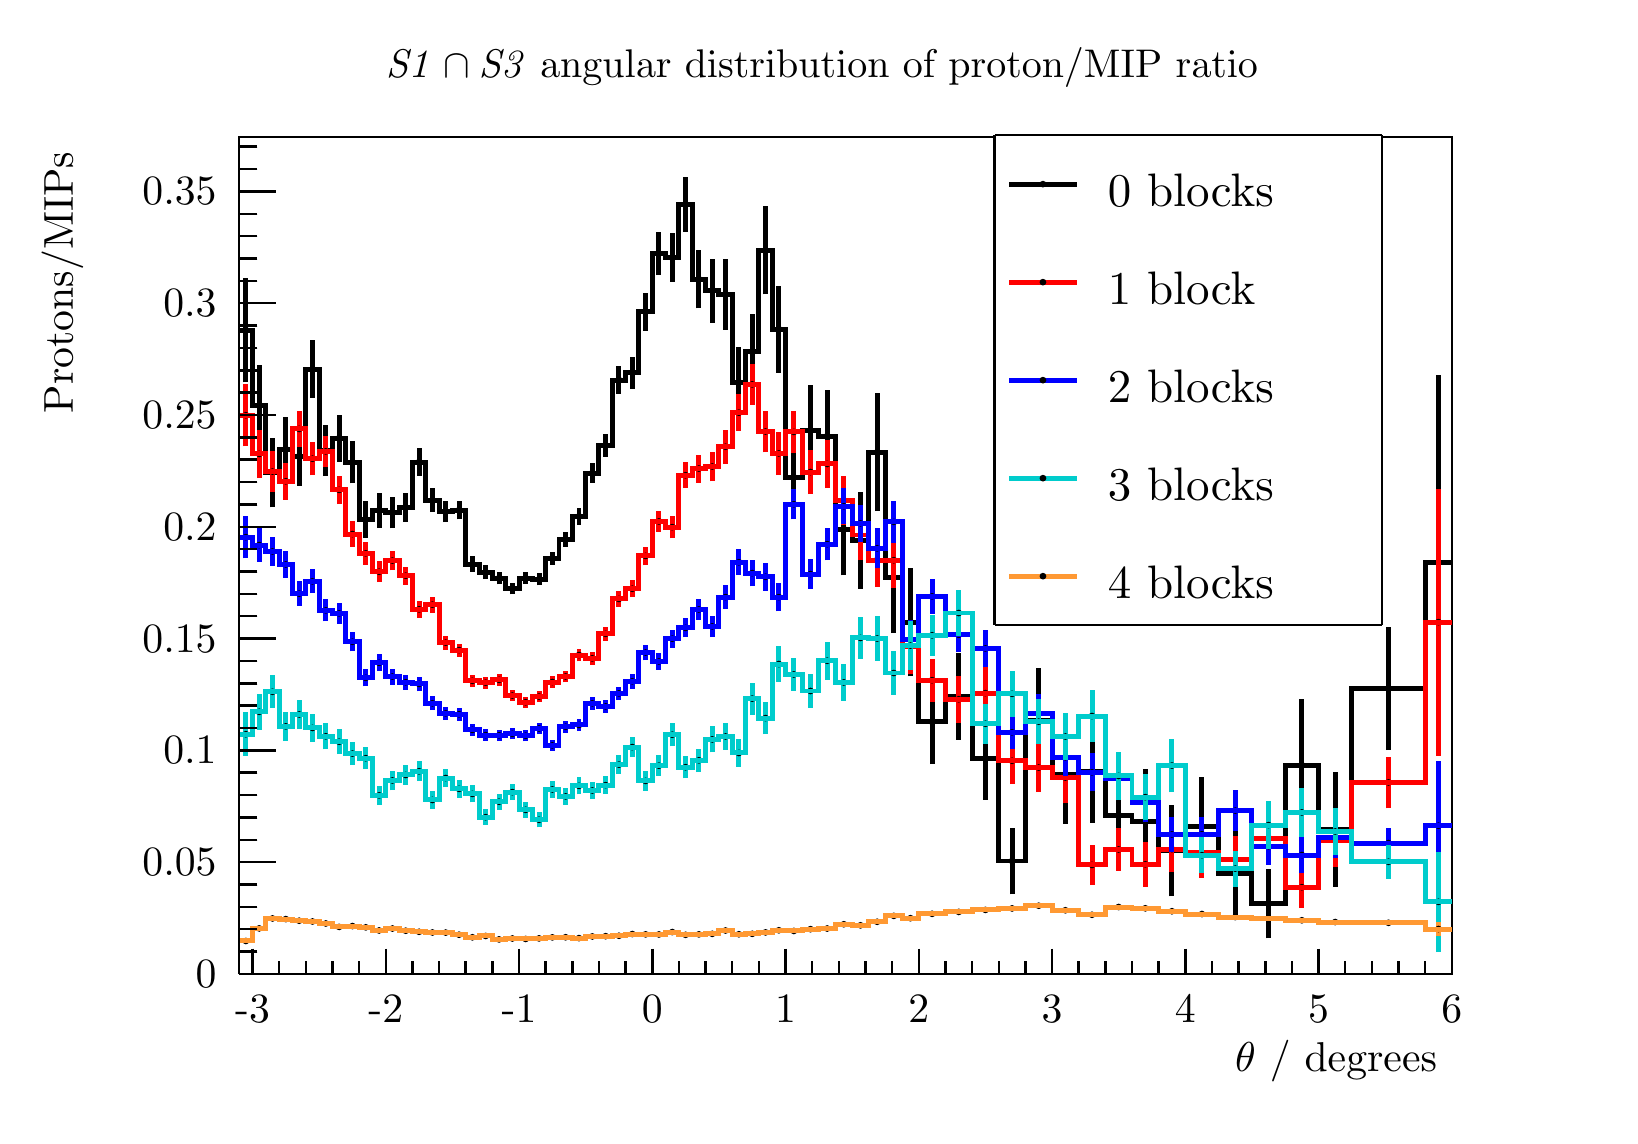
\begin{tikzpicture}
\pgfdeclareplotmark{cross} {
\pgfpathmoveto{\pgfpoint{-0.3\pgfplotmarksize}{\pgfplotmarksize}}
\pgfpathlineto{\pgfpoint{+0.3\pgfplotmarksize}{\pgfplotmarksize}}
\pgfpathlineto{\pgfpoint{+0.3\pgfplotmarksize}{0.3\pgfplotmarksize}}
\pgfpathlineto{\pgfpoint{+1\pgfplotmarksize}{0.3\pgfplotmarksize}}
\pgfpathlineto{\pgfpoint{+1\pgfplotmarksize}{-0.3\pgfplotmarksize}}
\pgfpathlineto{\pgfpoint{+0.3\pgfplotmarksize}{-0.3\pgfplotmarksize}}
\pgfpathlineto{\pgfpoint{+0.3\pgfplotmarksize}{-1.\pgfplotmarksize}}
\pgfpathlineto{\pgfpoint{-0.3\pgfplotmarksize}{-1.\pgfplotmarksize}}
\pgfpathlineto{\pgfpoint{-0.3\pgfplotmarksize}{-0.3\pgfplotmarksize}}
\pgfpathlineto{\pgfpoint{-1.\pgfplotmarksize}{-0.3\pgfplotmarksize}}
\pgfpathlineto{\pgfpoint{-1.\pgfplotmarksize}{0.3\pgfplotmarksize}}
\pgfpathlineto{\pgfpoint{-0.3\pgfplotmarksize}{0.3\pgfplotmarksize}}
\pgfpathclose
\pgfusepathqstroke
}
\pgfdeclareplotmark{cross*} {
\pgfpathmoveto{\pgfpoint{-0.3\pgfplotmarksize}{\pgfplotmarksize}}
\pgfpathlineto{\pgfpoint{+0.3\pgfplotmarksize}{\pgfplotmarksize}}
\pgfpathlineto{\pgfpoint{+0.3\pgfplotmarksize}{0.3\pgfplotmarksize}}
\pgfpathlineto{\pgfpoint{+1\pgfplotmarksize}{0.3\pgfplotmarksize}}
\pgfpathlineto{\pgfpoint{+1\pgfplotmarksize}{-0.3\pgfplotmarksize}}
\pgfpathlineto{\pgfpoint{+0.3\pgfplotmarksize}{-0.3\pgfplotmarksize}}
\pgfpathlineto{\pgfpoint{+0.3\pgfplotmarksize}{-1.\pgfplotmarksize}}
\pgfpathlineto{\pgfpoint{-0.3\pgfplotmarksize}{-1.\pgfplotmarksize}}
\pgfpathlineto{\pgfpoint{-0.3\pgfplotmarksize}{-0.3\pgfplotmarksize}}
\pgfpathlineto{\pgfpoint{-1.\pgfplotmarksize}{-0.3\pgfplotmarksize}}
\pgfpathlineto{\pgfpoint{-1.\pgfplotmarksize}{0.3\pgfplotmarksize}}
\pgfpathlineto{\pgfpoint{-0.3\pgfplotmarksize}{0.3\pgfplotmarksize}}
\pgfpathclose
\pgfusepathqfillstroke
}
\pgfdeclareplotmark{newstar} {
\pgfpathmoveto{\pgfqpoint{0pt}{\pgfplotmarksize}}
\pgfpathlineto{\pgfqpointpolar{44}{0.5\pgfplotmarksize}}
\pgfpathlineto{\pgfqpointpolar{18}{\pgfplotmarksize}}
\pgfpathlineto{\pgfqpointpolar{-20}{0.5\pgfplotmarksize}}
\pgfpathlineto{\pgfqpointpolar{-54}{\pgfplotmarksize}}
\pgfpathlineto{\pgfqpointpolar{-90}{0.5\pgfplotmarksize}}
\pgfpathlineto{\pgfqpointpolar{234}{\pgfplotmarksize}}
\pgfpathlineto{\pgfqpointpolar{198}{0.5\pgfplotmarksize}}
\pgfpathlineto{\pgfqpointpolar{162}{\pgfplotmarksize}}
\pgfpathlineto{\pgfqpointpolar{134}{0.5\pgfplotmarksize}}
\pgfpathclose
\pgfusepathqstroke
}
\pgfdeclareplotmark{newstar*} {
\pgfpathmoveto{\pgfqpoint{0pt}{\pgfplotmarksize}}
\pgfpathlineto{\pgfqpointpolar{44}{0.5\pgfplotmarksize}}
\pgfpathlineto{\pgfqpointpolar{18}{\pgfplotmarksize}}
\pgfpathlineto{\pgfqpointpolar{-20}{0.5\pgfplotmarksize}}
\pgfpathlineto{\pgfqpointpolar{-54}{\pgfplotmarksize}}
\pgfpathlineto{\pgfqpointpolar{-90}{0.5\pgfplotmarksize}}
\pgfpathlineto{\pgfqpointpolar{234}{\pgfplotmarksize}}
\pgfpathlineto{\pgfqpointpolar{198}{0.5\pgfplotmarksize}}
\pgfpathlineto{\pgfqpointpolar{162}{\pgfplotmarksize}}
\pgfpathlineto{\pgfqpointpolar{134}{0.5\pgfplotmarksize}}
\pgfpathclose
\pgfusepathqfillstroke
}
\definecolor{c}{rgb}{1,1,1};
\draw [color=c, fill=c] (0,0) rectangle (20,13.8048);
\draw [color=c, fill=c] (2.6,1.79463) rectangle (18,12.4243);
\definecolor{c}{rgb}{0,0,0};
\draw [c,line width=0.9] (2.6,1.79463) -- (2.6,12.4243) -- (18,12.4243) -- (18,1.79463) -- (2.6,1.79463);
\definecolor{c}{rgb}{1,1,1};
\draw [color=c, fill=c] (2.6,1.79463) rectangle (18,12.4243);
\definecolor{c}{rgb}{0,0,0};
\draw [c,line width=0.9] (2.6,1.79463) -- (2.6,12.4243) -- (18,12.4243) -- (18,1.79463) -- (2.6,1.79463);
\definecolor{c}{rgb}{0,0,0.6};
\draw [c,line width=0.9] (2.6,1.79463) -- (2.76923,1.79463) -- (2.76923,1.79463) -- (2.93846,1.79463) -- (2.93846,1.79463) -- (3.10769,1.79463) -- (3.10769,1.79463) -- (3.27692,1.79463) -- (3.27692,1.79463) -- (3.44615,1.79463) -- (3.44615,1.79463)
 -- (3.61538,1.79463) -- (3.61538,1.79463) -- (3.78462,1.79463) -- (3.78462,1.79463) -- (3.95385,1.79463) -- (3.95385,1.79463) -- (4.12308,1.79463) -- (4.12308,1.79463) -- (4.29231,1.79463) -- (4.29231,1.79463) -- (4.46154,1.79463) --
 (4.46154,1.79463) -- (4.63077,1.79463) -- (4.63077,1.79463) -- (4.8,1.79463) -- (4.8,1.79463) -- (4.96923,1.79463) -- (4.96923,1.79463) -- (5.13846,1.79463) -- (5.13846,1.79463) -- (5.30769,1.79463) -- (5.30769,1.79463) -- (5.47692,1.79463) --
 (5.47692,1.79463) -- (5.64615,1.79463) -- (5.64615,1.79463) -- (5.81538,1.79463) -- (5.81538,1.79463) -- (5.98462,1.79463) -- (5.98462,1.79463) -- (6.15385,1.79463) -- (6.15385,1.79463) -- (6.32308,1.79463) -- (6.32308,1.79463) -- (6.49231,1.79463)
 -- (6.49231,1.79463) -- (6.66154,1.79463) -- (6.66154,1.79463) -- (6.83077,1.79463) -- (6.83077,1.79463) -- (7,1.79463) -- (7,1.79463) -- (7.16923,1.79463) -- (7.16923,1.79463) -- (7.33846,1.79463) -- (7.33846,1.79463) -- (7.50769,1.79463) --
 (7.50769,1.79463) -- (7.67692,1.79463) -- (7.67692,1.79463) -- (7.84615,1.79463) -- (7.84615,1.79463) -- (8.01538,1.79463) -- (8.01538,1.79463) -- (8.18462,1.79463) -- (8.18462,1.79463) -- (8.35385,1.79463) -- (8.35385,1.79463) -- (8.52308,1.79463)
 -- (8.52308,1.79463) -- (8.69231,1.79463) -- (8.69231,1.79463) -- (8.86154,1.79463) -- (8.86154,1.79463) -- (9.03077,1.79463) -- (9.03077,1.79463) -- (9.2,1.79463) -- (9.2,1.79463) -- (9.36923,1.79463) -- (9.36923,1.79463) -- (9.53846,1.79463) --
 (9.53846,1.79463) -- (9.75,1.79463) -- (9.75,1.79463) -- (9.96154,1.79463) -- (9.96154,1.79463) -- (10.1731,1.79463) -- (10.1731,1.79463) -- (10.3846,1.79463) -- (10.3846,1.79463) -- (10.5962,1.79463) -- (10.5962,1.79463) -- (10.8077,1.79463) --
 (10.8077,1.79463) -- (11.0192,1.79463) -- (11.0192,1.79463) -- (11.2308,1.79463) -- (11.2308,1.79463) -- (11.5692,1.79463) -- (11.5692,1.79463) -- (11.9077,1.79463) -- (11.9077,1.79463) -- (12.2462,1.79463) -- (12.2462,1.79463) -- (12.5846,1.79463)
 -- (12.5846,1.79463) -- (12.9231,1.79463) -- (12.9231,1.79463) -- (13.2615,1.79463) -- (13.2615,1.79463) -- (13.6,1.79463) -- (13.6,1.79463) -- (13.9385,1.79463) -- (13.9385,1.79463) -- (14.2769,1.79463) -- (14.2769,1.79463) -- (14.6154,1.79463) --
 (14.6154,1.79463) -- (15.0385,1.79463) -- (15.0385,1.79463) -- (15.4615,1.79463) -- (15.4615,1.79463) -- (15.8846,1.79463) -- (15.8846,1.79463) -- (16.3077,1.79463) -- (16.3077,1.79463) -- (16.7308,1.79463) -- (16.7308,1.79463) -- (17.6615,1.79463)
 -- (17.6615,1.79463) -- (18,1.79463);
\definecolor{c}{rgb}{0,0,0};
\draw [c,line width=0.9] (2.6,1.79463) -- (18,1.79463);
\draw [c,line width=0.9] (2.76923,2.11352) -- (2.76923,1.79463);
\draw [c,line width=0.9] (3.10769,1.95407) -- (3.10769,1.79463);
\draw [c,line width=0.9] (3.44615,1.95407) -- (3.44615,1.79463);
\draw [c,line width=0.9] (3.78462,1.95407) -- (3.78462,1.79463);
\draw [c,line width=0.9] (4.12308,1.95407) -- (4.12308,1.79463);
\draw [c,line width=0.9] (4.46154,2.11352) -- (4.46154,1.79463);
\draw [c,line width=0.9] (4.8,1.95407) -- (4.8,1.79463);
\draw [c,line width=0.9] (5.13846,1.95407) -- (5.13846,1.79463);
\draw [c,line width=0.9] (5.47692,1.95407) -- (5.47692,1.79463);
\draw [c,line width=0.9] (5.81538,1.95407) -- (5.81538,1.79463);
\draw [c,line width=0.9] (6.15385,2.11352) -- (6.15385,1.79463);
\draw [c,line width=0.9] (6.49231,1.95407) -- (6.49231,1.79463);
\draw [c,line width=0.9] (6.83077,1.95407) -- (6.83077,1.79463);
\draw [c,line width=0.9] (7.16923,1.95407) -- (7.16923,1.79463);
\draw [c,line width=0.9] (7.50769,1.95407) -- (7.50769,1.79463);
\draw [c,line width=0.9] (7.84615,2.11352) -- (7.84615,1.79463);
\draw [c,line width=0.9] (8.18462,1.95407) -- (8.18462,1.79463);
\draw [c,line width=0.9] (8.52308,1.95407) -- (8.52308,1.79463);
\draw [c,line width=0.9] (8.86154,1.95407) -- (8.86154,1.79463);
\draw [c,line width=0.9] (9.2,1.95407) -- (9.2,1.79463);
\draw [c,line width=0.9] (9.53846,2.11352) -- (9.53846,1.79463);
\draw [c,line width=0.9] (9.87692,1.95407) -- (9.87692,1.79463);
\draw [c,line width=0.9] (10.2154,1.95407) -- (10.2154,1.79463);
\draw [c,line width=0.9] (10.5538,1.95407) -- (10.5538,1.79463);
\draw [c,line width=0.9] (10.8923,1.95407) -- (10.8923,1.79463);
\draw [c,line width=0.9] (11.2308,2.11352) -- (11.2308,1.79463);
\draw [c,line width=0.9] (11.5692,1.95407) -- (11.5692,1.79463);
\draw [c,line width=0.9] (11.9077,1.95407) -- (11.9077,1.79463);
\draw [c,line width=0.9] (12.2462,1.95407) -- (12.2462,1.79463);
\draw [c,line width=0.9] (12.5846,1.95407) -- (12.5846,1.79463);
\draw [c,line width=0.9] (12.9231,2.11352) -- (12.9231,1.79463);
\draw [c,line width=0.9] (13.2615,1.95407) -- (13.2615,1.79463);
\draw [c,line width=0.9] (13.6,1.95407) -- (13.6,1.79463);
\draw [c,line width=0.9] (13.9385,1.95407) -- (13.9385,1.79463);
\draw [c,line width=0.9] (14.2769,1.95407) -- (14.2769,1.79463);
\draw [c,line width=0.9] (14.6154,2.11352) -- (14.6154,1.79463);
\draw [c,line width=0.9] (14.9538,1.95407) -- (14.9538,1.79463);
\draw [c,line width=0.9] (15.2923,1.95407) -- (15.2923,1.79463);
\draw [c,line width=0.9] (15.6308,1.95407) -- (15.6308,1.79463);
\draw [c,line width=0.9] (15.9692,1.95407) -- (15.9692,1.79463);
\draw [c,line width=0.9] (16.3077,2.11352) -- (16.3077,1.79463);
\draw [c,line width=0.9] (16.6462,1.95407) -- (16.6462,1.79463);
\draw [c,line width=0.9] (16.9846,1.95407) -- (16.9846,1.79463);
\draw [c,line width=0.9] (17.3231,1.95407) -- (17.3231,1.79463);
\draw [c,line width=0.9] (17.6615,1.95407) -- (17.6615,1.79463);
\draw [c,line width=0.9] (18,2.11352) -- (18,1.79463);
\draw [c,line width=0.9] (2.76923,2.11352) -- (2.76923,1.79463);
\draw [anchor=base] (2.76923,1.17341) node[scale=1.50787, color=c, rotate=0]{-3};
\draw [anchor=base] (4.46154,1.17341) node[scale=1.50787, color=c, rotate=0]{-2};
\draw [anchor=base] (6.15385,1.17341) node[scale=1.50787, color=c, rotate=0]{-1};
\draw [anchor=base] (7.84615,1.17341) node[scale=1.50787, color=c, rotate=0]{0};
\draw [anchor=base] (9.53846,1.17341) node[scale=1.50787, color=c, rotate=0]{1};
\draw [anchor=base] (11.2308,1.17341) node[scale=1.50787, color=c, rotate=0]{2};
\draw [anchor=base] (12.9231,1.17341) node[scale=1.50787, color=c, rotate=0]{3};
\draw [anchor=base] (14.6154,1.17341) node[scale=1.50787, color=c, rotate=0]{4};
\draw [anchor=base] (16.3077,1.17341) node[scale=1.50787, color=c, rotate=0]{5};
\draw [anchor=base] (18,1.17341) node[scale=1.50787, color=c, rotate=0]{6};
\draw [anchor= east] (18,0.69024) node[scale=1.50787, color=c, rotate=0]{$\theta$ / degrees};
\draw [c,line width=0.9] (2.6,1.79463) -- (2.6,12.4243);
\draw [c,line width=0.9] (3.062,1.79463) -- (2.6,1.79463);
\draw [c,line width=0.9] (2.831,2.07854) -- (2.6,2.07854);
\draw [c,line width=0.9] (2.831,2.36246) -- (2.6,2.36246);
\draw [c,line width=0.9] (2.831,2.64638) -- (2.6,2.64638);
\draw [c,line width=0.9] (2.831,2.9303) -- (2.6,2.9303);
\draw [c,line width=0.9] (3.062,3.21421) -- (2.6,3.21421);
\draw [c,line width=0.9] (2.831,3.49813) -- (2.6,3.49813);
\draw [c,line width=0.9] (2.831,3.78205) -- (2.6,3.78205);
\draw [c,line width=0.9] (2.831,4.06597) -- (2.6,4.06597);
\draw [c,line width=0.9] (2.831,4.34988) -- (2.6,4.34988);
\draw [c,line width=0.9] (3.062,4.6338) -- (2.6,4.6338);
\draw [c,line width=0.9] (2.831,4.91772) -- (2.6,4.91772);
\draw [c,line width=0.9] (2.831,5.20164) -- (2.6,5.20164);
\draw [c,line width=0.9] (2.831,5.48555) -- (2.6,5.48555);
\draw [c,line width=0.9] (2.831,5.76947) -- (2.6,5.76947);
\draw [c,line width=0.9] (3.062,6.05339) -- (2.6,6.05339);
\draw [c,line width=0.9] (2.831,6.33731) -- (2.6,6.33731);
\draw [c,line width=0.9] (2.831,6.62122) -- (2.6,6.62122);
\draw [c,line width=0.9] (2.831,6.90514) -- (2.6,6.90514);
\draw [c,line width=0.9] (2.831,7.18906) -- (2.6,7.18906);
\draw [c,line width=0.9] (3.062,7.47298) -- (2.6,7.47298);
\draw [c,line width=0.9] (2.831,7.75689) -- (2.6,7.75689);
\draw [c,line width=0.9] (2.831,8.04081) -- (2.6,8.04081);
\draw [c,line width=0.9] (2.831,8.32473) -- (2.6,8.32473);
\draw [c,line width=0.9] (2.831,8.60865) -- (2.6,8.60865);
\draw [c,line width=0.9] (3.062,8.89256) -- (2.6,8.89256);
\draw [c,line width=0.9] (2.831,9.17648) -- (2.6,9.17648);
\draw [c,line width=0.9] (2.831,9.4604) -- (2.6,9.4604);
\draw [c,line width=0.9] (2.831,9.74432) -- (2.6,9.74432);
\draw [c,line width=0.9] (2.831,10.0282) -- (2.6,10.0282);
\draw [c,line width=0.9] (3.062,10.3122) -- (2.6,10.3122);
\draw [c,line width=0.9] (2.831,10.5961) -- (2.6,10.5961);
\draw [c,line width=0.9] (2.831,10.88) -- (2.6,10.88);
\draw [c,line width=0.9] (2.831,11.1639) -- (2.6,11.1639);
\draw [c,line width=0.9] (2.831,11.4478) -- (2.6,11.4478);
\draw [c,line width=0.9] (3.062,11.7317) -- (2.6,11.7317);
\draw [c,line width=0.9] (3.062,11.7317) -- (2.6,11.7317);
\draw [c,line width=0.9] (2.831,12.0157) -- (2.6,12.0157);
\draw [c,line width=0.9] (2.831,12.2996) -- (2.6,12.2996);
\draw [anchor= east] (2.5,1.79463) node[scale=1.50787, color=c, rotate=0]{0};
\draw [anchor= east] (2.5,3.21421) node[scale=1.50787, color=c, rotate=0]{0.05};
\draw [anchor= east] (2.5,4.6338) node[scale=1.50787, color=c, rotate=0]{0.1};
\draw [anchor= east] (2.5,6.05339) node[scale=1.50787, color=c, rotate=0]{0.15};
\draw [anchor= east] (2.5,7.47298) node[scale=1.50787, color=c, rotate=0]{0.2};
\draw [anchor= east] (2.5,8.89256) node[scale=1.50787, color=c, rotate=0]{0.25};
\draw [anchor= east] (2.5,10.3122) node[scale=1.50787, color=c, rotate=0]{0.3};
\draw [anchor= east] (2.5,11.7317) node[scale=1.50787, color=c, rotate=0]{0.35};
\draw [anchor= east] (0.355304,12.4243) node[scale=1.50787, color=c, rotate=90]{  Protons/MIPs};
\draw [c,line width=1.8] (2.68462,9.30634) -- (2.68462,9.97008);
\draw [c,line width=1.8] (2.68462,9.97008) -- (2.68462,10.6338);
\foreach \P in {(2.68462,9.97008)}{\draw[mark options={color=c,fill=c},mark size=2.402402pt,mark=*,mark size=1pt] plot coordinates {\P};}
\draw [c,line width=1.8] (2.85385,8.49736) -- (2.85385,9.01355);
\draw [c,line width=1.8] (2.85385,9.01355) -- (2.85385,9.52973);
\foreach \P in {(2.85385,9.01355)}{\draw[mark options={color=c,fill=c},mark size=2.402402pt,mark=*,mark size=1pt] plot coordinates {\P};}
\draw [c,line width=1.8] (3.02308,7.72066) -- (3.02308,8.15841);
\draw [c,line width=1.8] (3.02308,8.15841) -- (3.02308,8.59615);
\foreach \P in {(3.02308,8.15841)}{\draw[mark options={color=c,fill=c},mark size=2.402402pt,mark=*,mark size=1pt] plot coordinates {\P};}
\draw [c,line width=1.8] (3.19231,8.05064) -- (3.19231,8.45824);
\draw [c,line width=1.8] (3.19231,8.45824) -- (3.19231,8.86585);
\foreach \P in {(3.19231,8.45824)}{\draw[mark options={color=c,fill=c},mark size=2.402402pt,mark=*,mark size=1pt] plot coordinates {\P};}
\draw [c,line width=1.8] (3.36154,7.99502) -- (3.36154,8.36961);
\draw [c,line width=1.8] (3.36154,8.36961) -- (3.36154,8.7442);
\foreach \P in {(3.36154,8.36961)}{\draw[mark options={color=c,fill=c},mark size=2.402402pt,mark=*,mark size=1pt] plot coordinates {\P};}
\draw [c,line width=1.8] (3.53077,9.10979) -- (3.53077,9.47513);
\draw [c,line width=1.8] (3.53077,9.47513) -- (3.53077,9.84048);
\foreach \P in {(3.53077,9.47513)}{\draw[mark options={color=c,fill=c},mark size=2.402402pt,mark=*,mark size=1pt] plot coordinates {\P};}
\draw [c,line width=1.8] (3.7,8.11735) -- (3.7,8.4427);
\draw [c,line width=1.8] (3.7,8.4427) -- (3.7,8.76804);
\foreach \P in {(3.7,8.4427)}{\draw[mark options={color=c,fill=c},mark size=2.402402pt,mark=*,mark size=1pt] plot coordinates {\P};}
\draw [c,line width=1.8] (3.86923,8.29828) -- (3.86923,8.59788);
\draw [c,line width=1.8] (3.86923,8.59788) -- (3.86923,8.89747);
\foreach \P in {(3.86923,8.59788)}{\draw[mark options={color=c,fill=c},mark size=2.402402pt,mark=*,mark size=1pt] plot coordinates {\P};}
\draw [c,line width=1.8] (4.03846,8.02434) -- (4.03846,8.29309);
\draw [c,line width=1.8] (4.03846,8.29309) -- (4.03846,8.56183);
\foreach \P in {(4.03846,8.29309)}{\draw[mark options={color=c,fill=c},mark size=2.402402pt,mark=*,mark size=1pt] plot coordinates {\P};}
\draw [c,line width=1.8] (4.20769,7.33229) -- (4.20769,7.56705);
\draw [c,line width=1.8] (4.20769,7.56705) -- (4.20769,7.8018);
\foreach \P in {(4.20769,7.56705)}{\draw[mark options={color=c,fill=c},mark size=2.402402pt,mark=*,mark size=1pt] plot coordinates {\P};}
\draw [c,line width=1.8] (4.37692,7.4621) -- (4.37692,7.68137);
\draw [c,line width=1.8] (4.37692,7.68137) -- (4.37692,7.90064);
\foreach \P in {(4.37692,7.68137)}{\draw[mark options={color=c,fill=c},mark size=2.402402pt,mark=*,mark size=1pt] plot coordinates {\P};}
\draw [c,line width=1.8] (4.54615,7.45238) -- (4.54615,7.65157);
\draw [c,line width=1.8] (4.54615,7.65157) -- (4.54615,7.85076);
\foreach \P in {(4.54615,7.65157)}{\draw[mark options={color=c,fill=c},mark size=2.402402pt,mark=*,mark size=1pt] plot coordinates {\P};}
\draw [c,line width=1.8] (4.71538,7.53519) -- (4.71538,7.71947);
\draw [c,line width=1.8] (4.71538,7.71947) -- (4.71538,7.90374);
\foreach \P in {(4.71538,7.71947)}{\draw[mark options={color=c,fill=c},mark size=2.402402pt,mark=*,mark size=1pt] plot coordinates {\P};}
\draw [c,line width=1.8] (4.88462,8.12215) -- (4.88462,8.29549);
\draw [c,line width=1.8] (4.88462,8.29549) -- (4.88462,8.46883);
\foreach \P in {(4.88462,8.29549)}{\draw[mark options={color=c,fill=c},mark size=2.402402pt,mark=*,mark size=1pt] plot coordinates {\P};}
\draw [c,line width=1.8] (5.05385,7.65871) -- (5.05385,7.81125);
\draw [c,line width=1.8] (5.05385,7.81125) -- (5.05385,7.96379);
\foreach \P in {(5.05385,7.81125)}{\draw[mark options={color=c,fill=c},mark size=2.402402pt,mark=*,mark size=1pt] plot coordinates {\P};}
\draw [c,line width=1.8] (5.22308,7.53198) -- (5.22308,7.66585);
\draw [c,line width=1.8] (5.22308,7.66585) -- (5.22308,7.79972);
\foreach \P in {(5.22308,7.66585)}{\draw[mark options={color=c,fill=c},mark size=2.402402pt,mark=*,mark size=1pt] plot coordinates {\P};}
\draw [c,line width=1.8] (5.39231,7.56675) -- (5.39231,7.68444);
\draw [c,line width=1.8] (5.39231,7.68444) -- (5.39231,7.80214);
\foreach \P in {(5.39231,7.68444)}{\draw[mark options={color=c,fill=c},mark size=2.402402pt,mark=*,mark size=1pt] plot coordinates {\P};}
\draw [c,line width=1.8] (5.56154,6.90069) -- (5.56154,6.99883);
\draw [c,line width=1.8] (5.56154,6.99883) -- (5.56154,7.09697);
\foreach \P in {(5.56154,6.99883)}{\draw[mark options={color=c,fill=c},mark size=2.402402pt,mark=*,mark size=1pt] plot coordinates {\P};}
\draw [c,line width=1.8] (5.73077,6.80854) -- (5.73077,6.89512);
\draw [c,line width=1.8] (5.73077,6.89512) -- (5.73077,6.9817);
\foreach \P in {(5.73077,6.89512)}{\draw[mark options={color=c,fill=c},mark size=2.402402pt,mark=*,mark size=1pt] plot coordinates {\P};}
\draw [c,line width=1.8] (5.9,6.74235) -- (5.9,6.82131);
\draw [c,line width=1.8] (5.9,6.82131) -- (5.9,6.90027);
\foreach \P in {(5.9,6.82131)}{\draw[mark options={color=c,fill=c},mark size=2.402402pt,mark=*,mark size=1pt] plot coordinates {\P};}
\draw [c,line width=1.8] (6.06923,6.61586) -- (6.06923,6.68987);
\draw [c,line width=1.8] (6.06923,6.68987) -- (6.06923,6.76388);
\foreach \P in {(6.06923,6.68987)}{\draw[mark options={color=c,fill=c},mark size=2.402402pt,mark=*,mark size=1pt] plot coordinates {\P};}
\draw [c,line width=1.8] (6.23846,6.74776) -- (6.23846,6.82207);
\draw [c,line width=1.8] (6.23846,6.82207) -- (6.23846,6.89638);
\foreach \P in {(6.23846,6.82207)}{\draw[mark options={color=c,fill=c},mark size=2.402402pt,mark=*,mark size=1pt] plot coordinates {\P};}
\draw [c,line width=1.8] (6.40769,6.72859) -- (6.40769,6.80478);
\draw [c,line width=1.8] (6.40769,6.80478) -- (6.40769,6.88096);
\foreach \P in {(6.40769,6.80478)}{\draw[mark options={color=c,fill=c},mark size=2.402402pt,mark=*,mark size=1pt] plot coordinates {\P};}
\draw [c,line width=1.8] (6.57692,6.98887) -- (6.57692,7.07216);
\draw [c,line width=1.8] (6.57692,7.07216) -- (6.57692,7.15545);
\foreach \P in {(6.57692,7.07216)}{\draw[mark options={color=c,fill=c},mark size=2.402402pt,mark=*,mark size=1pt] plot coordinates {\P};}
\draw [c,line width=1.8] (6.74615,7.21777) -- (6.74615,7.31138);
\draw [c,line width=1.8] (6.74615,7.31138) -- (6.74615,7.40499);
\foreach \P in {(6.74615,7.31138)}{\draw[mark options={color=c,fill=c},mark size=2.402402pt,mark=*,mark size=1pt] plot coordinates {\P};}
\draw [c,line width=1.8] (6.91538,7.50065) -- (6.91538,7.60619);
\draw [c,line width=1.8] (6.91538,7.60619) -- (6.91538,7.71173);
\foreach \P in {(6.91538,7.60619)}{\draw[mark options={color=c,fill=c},mark size=2.402402pt,mark=*,mark size=1pt] plot coordinates {\P};}
\draw [c,line width=1.8] (7.08462,8.03336) -- (7.08462,8.15574);
\draw [c,line width=1.8] (7.08462,8.15574) -- (7.08462,8.27812);
\foreach \P in {(7.08462,8.15574)}{\draw[mark options={color=c,fill=c},mark size=2.402402pt,mark=*,mark size=1pt] plot coordinates {\P};}
\draw [c,line width=1.8] (7.25385,8.36273) -- (7.25385,8.50567);
\draw [c,line width=1.8] (7.25385,8.50567) -- (7.25385,8.64861);
\foreach \P in {(7.25385,8.50567)}{\draw[mark options={color=c,fill=c},mark size=2.402402pt,mark=*,mark size=1pt] plot coordinates {\P};}
\draw [c,line width=1.8] (7.42308,9.16474) -- (7.42308,9.33698);
\draw [c,line width=1.8] (7.42308,9.33698) -- (7.42308,9.50921);
\foreach \P in {(7.42308,9.33698)}{\draw[mark options={color=c,fill=c},mark size=2.402402pt,mark=*,mark size=1pt] plot coordinates {\P};}
\draw [c,line width=1.8] (7.59231,9.22735) -- (7.59231,9.42869);
\draw [c,line width=1.8] (7.59231,9.42869) -- (7.59231,9.63002);
\foreach \P in {(7.59231,9.42869)}{\draw[mark options={color=c,fill=c},mark size=2.402402pt,mark=*,mark size=1pt] plot coordinates {\P};}
\draw [c,line width=1.8] (7.76154,9.96284) -- (7.76154,10.2029);
\draw [c,line width=1.8] (7.76154,10.2029) -- (7.76154,10.4429);
\foreach \P in {(7.76154,10.2029)}{\draw[mark options={color=c,fill=c},mark size=2.402402pt,mark=*,mark size=1pt] plot coordinates {\P};}
\draw [c,line width=1.8] (7.93077,10.6703) -- (7.93077,10.9432);
\draw [c,line width=1.8] (7.93077,10.9432) -- (7.93077,11.2162);
\foreach \P in {(7.93077,10.9432)}{\draw[mark options={color=c,fill=c},mark size=2.402402pt,mark=*,mark size=1pt] plot coordinates {\P};}
\draw [c,line width=1.8] (8.1,10.5841) -- (8.1,10.8914);
\draw [c,line width=1.8] (8.1,10.8914) -- (8.1,11.1986);
\foreach \P in {(8.1,10.8914)}{\draw[mark options={color=c,fill=c},mark size=2.402402pt,mark=*,mark size=1pt] plot coordinates {\P};}
\draw [c,line width=1.8] (8.26923,11.2169) -- (8.26923,11.5675);
\draw [c,line width=1.8] (8.26923,11.5675) -- (8.26923,11.9182);
\foreach \P in {(8.26923,11.5675)}{\draw[mark options={color=c,fill=c},mark size=2.402402pt,mark=*,mark size=1pt] plot coordinates {\P};}
\draw [c,line width=1.8] (8.43846,10.2481) -- (8.43846,10.617);
\draw [c,line width=1.8] (8.43846,10.617) -- (8.43846,10.9859);
\foreach \P in {(8.43846,10.617)}{\draw[mark options={color=c,fill=c},mark size=2.402402pt,mark=*,mark size=1pt] plot coordinates {\P};}
\draw [c,line width=1.8] (8.60769,10.0646) -- (8.60769,10.4704);
\draw [c,line width=1.8] (8.60769,10.4704) -- (8.60769,10.8763);
\foreach \P in {(8.60769,10.4704)}{\draw[mark options={color=c,fill=c},mark size=2.402402pt,mark=*,mark size=1pt] plot coordinates {\P};}
\draw [c,line width=1.8] (8.77692,9.97668) -- (8.77692,10.4251);
\draw [c,line width=1.8] (8.77692,10.4251) -- (8.77692,10.8734);
\foreach \P in {(8.77692,10.4251)}{\draw[mark options={color=c,fill=c},mark size=2.402402pt,mark=*,mark size=1pt] plot coordinates {\P};}
\draw [c,line width=1.8] (8.94615,8.86056) -- (8.94615,9.30864);
\draw [c,line width=1.8] (8.94615,9.30864) -- (8.94615,9.75671);
\foreach \P in {(8.94615,9.30864)}{\draw[mark options={color=c,fill=c},mark size=2.402402pt,mark=*,mark size=1pt] plot coordinates {\P};}
\draw [c,line width=1.8] (9.11538,9.20815) -- (9.11538,9.69291);
\draw [c,line width=1.8] (9.11538,9.69291) -- (9.11538,10.1777);
\foreach \P in {(9.11538,9.69291)}{\draw[mark options={color=c,fill=c},mark size=2.402402pt,mark=*,mark size=1pt] plot coordinates {\P};}
\draw [c,line width=1.8] (9.28462,10.4244) -- (9.28462,10.985);
\draw [c,line width=1.8] (9.28462,10.985) -- (9.28462,11.5455);
\foreach \P in {(9.28462,10.985)}{\draw[mark options={color=c,fill=c},mark size=2.402402pt,mark=*,mark size=1pt] plot coordinates {\P};}
\draw [c,line width=1.8] (9.45385,9.43204) -- (9.45385,9.98242);
\draw [c,line width=1.8] (9.45385,9.98242) -- (9.45385,10.5328);
\foreach \P in {(9.45385,9.98242)}{\draw[mark options={color=c,fill=c},mark size=2.402402pt,mark=*,mark size=1pt] plot coordinates {\P};}
\draw [c,line width=1.8] (9.64423,7.61559) -- (9.64423,8.10081);
\draw [c,line width=1.8] (9.64423,8.10081) -- (9.64423,8.58604);
\foreach \P in {(9.64423,8.10081)}{\draw[mark options={color=c,fill=c},mark size=2.402402pt,mark=*,mark size=1pt] plot coordinates {\P};}
\draw [c,line width=1.8] (9.85577,8.11155) -- (9.85577,8.69138);
\draw [c,line width=1.8] (9.85577,8.69138) -- (9.85577,9.27121);
\foreach \P in {(9.85577,8.69138)}{\draw[mark options={color=c,fill=c},mark size=2.402402pt,mark=*,mark size=1pt] plot coordinates {\P};}
\draw [c,line width=1.8] (10.0673,8.04672) -- (10.0673,8.62551);
\draw [c,line width=1.8] (10.0673,8.62551) -- (10.0673,9.20431);
\foreach \P in {(10.0673,8.62551)}{\draw[mark options={color=c,fill=c},mark size=2.402402pt,mark=*,mark size=1pt] plot coordinates {\P};}
\draw [c,line width=1.8] (10.2788,6.85722) -- (10.2788,7.4442);
\draw [c,line width=1.8] (10.2788,7.4442) -- (10.2788,8.03118);
\foreach \P in {(10.2788,7.4442)}{\draw[mark options={color=c,fill=c},mark size=2.402402pt,mark=*,mark size=1pt] plot coordinates {\P};}
\draw [c,line width=1.8] (10.4904,6.68422) -- (10.4904,7.29976);
\draw [c,line width=1.8] (10.4904,7.29976) -- (10.4904,7.9153);
\foreach \P in {(10.4904,7.29976)}{\draw[mark options={color=c,fill=c},mark size=2.402402pt,mark=*,mark size=1pt] plot coordinates {\P};}
\draw [c,line width=1.8] (10.7019,7.67136) -- (10.7019,8.41897);
\draw [c,line width=1.8] (10.7019,8.41897) -- (10.7019,9.16657);
\foreach \P in {(10.7019,8.41897)}{\draw[mark options={color=c,fill=c},mark size=2.402402pt,mark=*,mark size=1pt] plot coordinates {\P};}
\draw [c,line width=1.8] (10.9135,6.1232) -- (10.9135,6.83123);
\draw [c,line width=1.8] (10.9135,6.83123) -- (10.9135,7.53926);
\foreach \P in {(10.9135,6.83123)}{\draw[mark options={color=c,fill=c},mark size=2.402402pt,mark=*,mark size=1pt] plot coordinates {\P};}
\draw [c,line width=1.8] (11.125,5.57256) -- (11.125,6.26237);
\draw [c,line width=1.8] (11.125,6.26237) -- (11.125,6.95218);
\foreach \P in {(11.125,6.26237)}{\draw[mark options={color=c,fill=c},mark size=2.402402pt,mark=*,mark size=1pt] plot coordinates {\P};}
\draw [c,line width=1.8] (11.4,4.45921) -- (11.4,4.99664);
\draw [c,line width=1.8] (11.4,4.99664) -- (11.4,5.53408);
\foreach \P in {(11.4,4.99664)}{\draw[mark options={color=c,fill=c},mark size=2.402402pt,mark=*,mark size=1pt] plot coordinates {\P};}
\draw [c,line width=1.8] (11.7385,4.7668) -- (11.7385,5.318);
\draw [c,line width=1.8] (11.7385,5.318) -- (11.7385,5.86921);
\foreach \P in {(11.7385,5.318)}{\draw[mark options={color=c,fill=c},mark size=2.402402pt,mark=*,mark size=1pt] plot coordinates {\P};}
\draw [c,line width=1.8] (12.0769,4.00654) -- (12.0769,4.53057);
\draw [c,line width=1.8] (12.0769,4.53057) -- (12.0769,5.05461);
\foreach \P in {(12.0769,4.53057)}{\draw[mark options={color=c,fill=c},mark size=2.402402pt,mark=*,mark size=1pt] plot coordinates {\P};}
\draw [c,line width=1.8] (12.4154,2.80479) -- (12.4154,3.22846);
\draw [c,line width=1.8] (12.4154,3.22846) -- (12.4154,3.65213);
\foreach \P in {(12.4154,3.22846)}{\draw[mark options={color=c,fill=c},mark size=2.402402pt,mark=*,mark size=1pt] plot coordinates {\P};}
\draw [c,line width=1.8] (12.7538,4.34921) -- (12.7538,5.01384);
\draw [c,line width=1.8] (12.7538,5.01384) -- (12.7538,5.67847);
\foreach \P in {(12.7538,5.01384)}{\draw[mark options={color=c,fill=c},mark size=2.402402pt,mark=*,mark size=1pt] plot coordinates {\P};}
\draw [c,line width=1.8] (13.0923,3.70333) -- (13.0923,4.33019);
\draw [c,line width=1.8] (13.0923,4.33019) -- (13.0923,4.95704);
\foreach \P in {(13.0923,4.33019)}{\draw[mark options={color=c,fill=c},mark size=2.402402pt,mark=*,mark size=1pt] plot coordinates {\P};}
\draw [c,line width=1.8] (13.4308,3.71119) -- (13.4308,4.36923);
\draw [c,line width=1.8] (13.4308,4.36923) -- (13.4308,5.02727);
\foreach \P in {(13.4308,4.36923)}{\draw[mark options={color=c,fill=c},mark size=2.402402pt,mark=*,mark size=1pt] plot coordinates {\P};}
\draw [c,line width=1.8] (13.7692,3.19368) -- (13.7692,3.81192);
\draw [c,line width=1.8] (13.7692,3.81192) -- (13.7692,4.43016);
\foreach \P in {(13.7692,3.81192)}{\draw[mark options={color=c,fill=c},mark size=2.402402pt,mark=*,mark size=1pt] plot coordinates {\P};}
\draw [c,line width=1.8] (14.1077,3.07144) -- (14.1077,3.73547);
\draw [c,line width=1.8] (14.1077,3.73547) -- (14.1077,4.39949);
\foreach \P in {(14.1077,3.73547)}{\draw[mark options={color=c,fill=c},mark size=2.402402pt,mark=*,mark size=1pt] plot coordinates {\P};}
\draw [c,line width=1.8] (14.4462,2.77998) -- (14.4462,3.35949);
\draw [c,line width=1.8] (14.4462,3.35949) -- (14.4462,3.93899);
\foreach \P in {(14.4462,3.35949)}{\draw[mark options={color=c,fill=c},mark size=2.402402pt,mark=*,mark size=1pt] plot coordinates {\P};}
\draw [c,line width=1.8] (14.8269,3.0208) -- (14.8269,3.66085);
\draw [c,line width=1.8] (14.8269,3.66085) -- (14.8269,4.3009);
\foreach \P in {(14.8269,3.66085)}{\draw[mark options={color=c,fill=c},mark size=2.402402pt,mark=*,mark size=1pt] plot coordinates {\P};}
\draw [c,line width=1.8] (15.25,2.5074) -- (15.25,3.06784);
\draw [c,line width=1.8] (15.25,3.06784) -- (15.25,3.62827);
\foreach \P in {(15.25,3.06784)}{\draw[mark options={color=c,fill=c},mark size=2.402402pt,mark=*,mark size=1pt] plot coordinates {\P};}
\draw [c,line width=1.8] (15.6731,2.24725) -- (15.6731,2.68774);
\draw [c,line width=1.8] (15.6731,2.68774) -- (15.6731,3.12823);
\foreach \P in {(15.6731,2.68774)}{\draw[mark options={color=c,fill=c},mark size=2.402402pt,mark=*,mark size=1pt] plot coordinates {\P};}
\draw [c,line width=1.8] (16.0962,3.60273) -- (16.0962,4.44549);
\draw [c,line width=1.8] (16.0962,4.44549) -- (16.0962,5.28825);
\foreach \P in {(16.0962,4.44549)}{\draw[mark options={color=c,fill=c},mark size=2.402402pt,mark=*,mark size=1pt] plot coordinates {\P};}
\draw [c,line width=1.8] (16.5192,2.90442) -- (16.5192,3.6312);
\draw [c,line width=1.8] (16.5192,3.6312) -- (16.5192,4.35798);
\foreach \P in {(16.5192,3.6312)}{\draw[mark options={color=c,fill=c},mark size=2.402402pt,mark=*,mark size=1pt] plot coordinates {\P};}
\draw [c,line width=1.8] (17.1962,4.63566) -- (17.1962,5.41617);
\draw [c,line width=1.8] (17.1962,5.41617) -- (17.1962,6.19669);
\foreach \P in {(17.1962,5.41617)}{\draw[mark options={color=c,fill=c},mark size=2.402402pt,mark=*,mark size=1pt] plot coordinates {\P};}
\draw [c,line width=1.8] (17.8308,4.63996) -- (17.8308,7.01988);
\draw [c,line width=1.8] (17.8308,7.01988) -- (17.8308,9.39979);
\foreach \P in {(17.8308,7.01988)}{\draw[mark options={color=c,fill=c},mark size=2.402402pt,mark=*,mark size=1pt] plot coordinates {\P};}
\draw [c,line width=1.8] (2.6,9.97008) -- (2.76923,9.97008) -- (2.76923,9.01355) -- (2.93846,9.01355) -- (2.93846,8.15841) -- (3.10769,8.15841) -- (3.10769,8.45824) -- (3.27692,8.45824) -- (3.27692,8.36961) -- (3.44615,8.36961) -- (3.44615,9.47513)
 -- (3.61538,9.47513) -- (3.61538,8.4427) -- (3.78462,8.4427) -- (3.78462,8.59788) -- (3.95385,8.59788) -- (3.95385,8.29309) -- (4.12308,8.29309) -- (4.12308,7.56705) -- (4.29231,7.56705) -- (4.29231,7.68137) -- (4.46154,7.68137) -- (4.46154,7.65157)
 -- (4.63077,7.65157) -- (4.63077,7.71947) -- (4.8,7.71947) -- (4.8,8.29549) -- (4.96923,8.29549) -- (4.96923,7.81125) -- (5.13846,7.81125) -- (5.13846,7.66585) -- (5.30769,7.66585) -- (5.30769,7.68444) -- (5.47692,7.68444) -- (5.47692,6.99883) --
 (5.64615,6.99883) -- (5.64615,6.89512) -- (5.81538,6.89512) -- (5.81538,6.82131) -- (5.98462,6.82131) -- (5.98462,6.68987) -- (6.15385,6.68987) -- (6.15385,6.82207) -- (6.32308,6.82207) -- (6.32308,6.80478) -- (6.49231,6.80478) -- (6.49231,7.07216)
 -- (6.66154,7.07216) -- (6.66154,7.31138) -- (6.83077,7.31138) -- (6.83077,7.60619) -- (7,7.60619) -- (7,8.15574) -- (7.16923,8.15574) -- (7.16923,8.50567) -- (7.33846,8.50567) -- (7.33846,9.33698) -- (7.50769,9.33698) -- (7.50769,9.42869) --
 (7.67692,9.42869) -- (7.67692,10.2029) -- (7.84615,10.2029) -- (7.84615,10.9432) -- (8.01538,10.9432) -- (8.01538,10.8914) -- (8.18462,10.8914) -- (8.18462,11.5675) -- (8.35385,11.5675) -- (8.35385,10.617) -- (8.52308,10.617) -- (8.52308,10.4704) --
 (8.69231,10.4704) -- (8.69231,10.4251) -- (8.86154,10.4251) -- (8.86154,9.30864) -- (9.03077,9.30864) -- (9.03077,9.69291) -- (9.2,9.69291) -- (9.2,10.985) -- (9.36923,10.985) -- (9.36923,9.98242) -- (9.53846,9.98242) -- (9.53846,8.10081) --
 (9.75,8.10081) -- (9.75,8.69138) -- (9.96154,8.69138) -- (9.96154,8.62551) -- (10.1731,8.62551) -- (10.1731,7.4442) -- (10.3846,7.4442) -- (10.3846,7.29976) -- (10.5962,7.29976) -- (10.5962,8.41897) -- (10.8077,8.41897) -- (10.8077,6.83123) --
 (11.0192,6.83123) -- (11.0192,6.26237) -- (11.2308,6.26237) -- (11.2308,4.99664) -- (11.5692,4.99664) -- (11.5692,5.318) -- (11.9077,5.318) -- (11.9077,4.53057) -- (12.2462,4.53057) -- (12.2462,3.22846) -- (12.5846,3.22846) -- (12.5846,5.01384) --
 (12.9231,5.01384) -- (12.9231,4.33019) -- (13.2615,4.33019) -- (13.2615,4.36923) -- (13.6,4.36923) -- (13.6,3.81192) -- (13.9385,3.81192) -- (13.9385,3.73547) -- (14.2769,3.73547) -- (14.2769,3.35949) -- (14.6154,3.35949) -- (14.6154,3.66085) --
 (15.0385,3.66085) -- (15.0385,3.06784) -- (15.4615,3.06784) -- (15.4615,2.68774) -- (15.8846,2.68774) -- (15.8846,4.44549) -- (16.3077,4.44549) -- (16.3077,3.6312) -- (16.7308,3.6312) -- (16.7308,5.41617) -- (17.6615,5.41617) -- (17.6615,7.01988) --
 (18,7.01988);
\definecolor{c}{rgb}{1,0,0};
\draw [c,line width=1.8] (2.68462,8.49513) -- (2.68462,8.89);
\draw [c,line width=1.8] (2.68462,8.89) -- (2.68462,9.28487);
\definecolor{c}{rgb}{0,0,0};
\foreach \P in {(2.68462,8.89)}{\draw[mark options={color=c,fill=c},mark size=2.402402pt,mark=*,mark size=1pt] plot coordinates {\P};}
\definecolor{c}{rgb}{1,0,0};
\draw [c,line width=1.8] (2.85385,8.09206) -- (2.85385,8.39823);
\draw [c,line width=1.8] (2.85385,8.39823) -- (2.85385,8.70441);
\definecolor{c}{rgb}{0,0,0};
\foreach \P in {(2.85385,8.39823)}{\draw[mark options={color=c,fill=c},mark size=2.402402pt,mark=*,mark size=1pt] plot coordinates {\P};}
\definecolor{c}{rgb}{1,0,0};
\draw [c,line width=1.8] (3.02308,7.91212) -- (3.02308,8.17432);
\draw [c,line width=1.8] (3.02308,8.17432) -- (3.02308,8.43652);
\definecolor{c}{rgb}{0,0,0};
\foreach \P in {(3.02308,8.17432)}{\draw[mark options={color=c,fill=c},mark size=2.402402pt,mark=*,mark size=1pt] plot coordinates {\P};}
\definecolor{c}{rgb}{1,0,0};
\draw [c,line width=1.8] (3.19231,7.81361) -- (3.19231,8.05101);
\draw [c,line width=1.8] (3.19231,8.05101) -- (3.19231,8.28841);
\definecolor{c}{rgb}{0,0,0};
\foreach \P in {(3.19231,8.05101)}{\draw[mark options={color=c,fill=c},mark size=2.402402pt,mark=*,mark size=1pt] plot coordinates {\P};}
\definecolor{c}{rgb}{1,0,0};
\draw [c,line width=1.8] (3.36154,8.48496) -- (3.36154,8.71586);
\draw [c,line width=1.8] (3.36154,8.71586) -- (3.36154,8.94677);
\definecolor{c}{rgb}{0,0,0};
\foreach \P in {(3.36154,8.71586)}{\draw[mark options={color=c,fill=c},mark size=2.402402pt,mark=*,mark size=1pt] plot coordinates {\P};}
\definecolor{c}{rgb}{1,0,0};
\draw [c,line width=1.8] (3.53077,8.12625) -- (3.53077,8.3375);
\draw [c,line width=1.8] (3.53077,8.3375) -- (3.53077,8.54875);
\definecolor{c}{rgb}{0,0,0};
\foreach \P in {(3.53077,8.3375)}{\draw[mark options={color=c,fill=c},mark size=2.402402pt,mark=*,mark size=1pt] plot coordinates {\P};}
\definecolor{c}{rgb}{1,0,0};
\draw [c,line width=1.8] (3.7,8.23062) -- (3.7,8.43064);
\draw [c,line width=1.8] (3.7,8.43064) -- (3.7,8.63066);
\definecolor{c}{rgb}{0,0,0};
\foreach \P in {(3.7,8.43064)}{\draw[mark options={color=c,fill=c},mark size=2.402402pt,mark=*,mark size=1pt] plot coordinates {\P};}
\definecolor{c}{rgb}{1,0,0};
\draw [c,line width=1.8] (3.86923,7.76146) -- (3.86923,7.94177);
\draw [c,line width=1.8] (3.86923,7.94177) -- (3.86923,8.12209);
\definecolor{c}{rgb}{0,0,0};
\foreach \P in {(3.86923,7.94177)}{\draw[mark options={color=c,fill=c},mark size=2.402402pt,mark=*,mark size=1pt] plot coordinates {\P};}
\definecolor{c}{rgb}{1,0,0};
\draw [c,line width=1.8] (4.03846,7.22024) -- (4.03846,7.38065);
\draw [c,line width=1.8] (4.03846,7.38065) -- (4.03846,7.54105);
\definecolor{c}{rgb}{0,0,0};
\foreach \P in {(4.03846,7.38065)}{\draw[mark options={color=c,fill=c},mark size=2.402402pt,mark=*,mark size=1pt] plot coordinates {\P};}
\definecolor{c}{rgb}{1,0,0};
\draw [c,line width=1.8] (4.20769,6.98925) -- (4.20769,7.13608);
\draw [c,line width=1.8] (4.20769,7.13608) -- (4.20769,7.28291);
\definecolor{c}{rgb}{0,0,0};
\foreach \P in {(4.20769,7.13608)}{\draw[mark options={color=c,fill=c},mark size=2.402402pt,mark=*,mark size=1pt] plot coordinates {\P};}
\definecolor{c}{rgb}{1,0,0};
\draw [c,line width=1.8] (4.37692,6.76972) -- (4.37692,6.90198);
\draw [c,line width=1.8] (4.37692,6.90198) -- (4.37692,7.03424);
\definecolor{c}{rgb}{0,0,0};
\foreach \P in {(4.37692,6.90198)}{\draw[mark options={color=c,fill=c},mark size=2.402402pt,mark=*,mark size=1pt] plot coordinates {\P};}
\definecolor{c}{rgb}{1,0,0};
\draw [c,line width=1.8] (4.54615,6.91865) -- (4.54615,7.04367);
\draw [c,line width=1.8] (4.54615,7.04367) -- (4.54615,7.16869);
\definecolor{c}{rgb}{0,0,0};
\foreach \P in {(4.54615,7.04367)}{\draw[mark options={color=c,fill=c},mark size=2.402402pt,mark=*,mark size=1pt] plot coordinates {\P};}
\definecolor{c}{rgb}{1,0,0};
\draw [c,line width=1.8] (4.71538,6.73542) -- (4.71538,6.8517);
\draw [c,line width=1.8] (4.71538,6.8517) -- (4.71538,6.96798);
\definecolor{c}{rgb}{0,0,0};
\foreach \P in {(4.71538,6.8517)}{\draw[mark options={color=c,fill=c},mark size=2.402402pt,mark=*,mark size=1pt] plot coordinates {\P};}
\definecolor{c}{rgb}{1,0,0};
\draw [c,line width=1.8] (4.88462,6.31956) -- (4.88462,6.42477);
\draw [c,line width=1.8] (4.88462,6.42477) -- (4.88462,6.52997);
\definecolor{c}{rgb}{0,0,0};
\foreach \P in {(4.88462,6.42477)}{\draw[mark options={color=c,fill=c},mark size=2.402402pt,mark=*,mark size=1pt] plot coordinates {\P};}
\definecolor{c}{rgb}{1,0,0};
\draw [c,line width=1.8] (5.05385,6.38426) -- (5.05385,6.48415);
\draw [c,line width=1.8] (5.05385,6.48415) -- (5.05385,6.58405);
\definecolor{c}{rgb}{0,0,0};
\foreach \P in {(5.05385,6.48415)}{\draw[mark options={color=c,fill=c},mark size=2.402402pt,mark=*,mark size=1pt] plot coordinates {\P};}
\definecolor{c}{rgb}{1,0,0};
\draw [c,line width=1.8] (5.22308,5.91141) -- (5.22308,6.0014);
\draw [c,line width=1.8] (5.22308,6.0014) -- (5.22308,6.09139);
\definecolor{c}{rgb}{0,0,0};
\foreach \P in {(5.22308,6.0014)}{\draw[mark options={color=c,fill=c},mark size=2.402402pt,mark=*,mark size=1pt] plot coordinates {\P};}
\definecolor{c}{rgb}{1,0,0};
\draw [c,line width=1.8] (5.39231,5.82277) -- (5.39231,5.90675);
\draw [c,line width=1.8] (5.39231,5.90675) -- (5.39231,5.99073);
\definecolor{c}{rgb}{0,0,0};
\foreach \P in {(5.39231,5.90675)}{\draw[mark options={color=c,fill=c},mark size=2.402402pt,mark=*,mark size=1pt] plot coordinates {\P};}
\definecolor{c}{rgb}{1,0,0};
\draw [c,line width=1.8] (5.56154,5.43958) -- (5.56154,5.51665);
\draw [c,line width=1.8] (5.56154,5.51665) -- (5.56154,5.59371);
\definecolor{c}{rgb}{0,0,0};
\foreach \P in {(5.56154,5.51665)}{\draw[mark options={color=c,fill=c},mark size=2.402402pt,mark=*,mark size=1pt] plot coordinates {\P};}
\definecolor{c}{rgb}{1,0,0};
\draw [c,line width=1.8] (5.73077,5.41915) -- (5.73077,5.49316);
\draw [c,line width=1.8] (5.73077,5.49316) -- (5.73077,5.56718);
\definecolor{c}{rgb}{0,0,0};
\foreach \P in {(5.73077,5.49316)}{\draw[mark options={color=c,fill=c},mark size=2.402402pt,mark=*,mark size=1pt] plot coordinates {\P};}
\definecolor{c}{rgb}{1,0,0};
\draw [c,line width=1.8] (5.9,5.45711) -- (5.9,5.52911);
\draw [c,line width=1.8] (5.9,5.52911) -- (5.9,5.60111);
\definecolor{c}{rgb}{0,0,0};
\foreach \P in {(5.9,5.52911)}{\draw[mark options={color=c,fill=c},mark size=2.402402pt,mark=*,mark size=1pt] plot coordinates {\P};}
\definecolor{c}{rgb}{1,0,0};
\draw [c,line width=1.8] (6.06923,5.26029) -- (6.06923,5.32951);
\draw [c,line width=1.8] (6.06923,5.32951) -- (6.06923,5.39873);
\definecolor{c}{rgb}{0,0,0};
\foreach \P in {(6.06923,5.32951)}{\draw[mark options={color=c,fill=c},mark size=2.402402pt,mark=*,mark size=1pt] plot coordinates {\P};}
\definecolor{c}{rgb}{1,0,0};
\draw [c,line width=1.8] (6.23846,5.17685) -- (6.23846,5.24448);
\draw [c,line width=1.8] (6.23846,5.24448) -- (6.23846,5.31211);
\definecolor{c}{rgb}{0,0,0};
\foreach \P in {(6.23846,5.24448)}{\draw[mark options={color=c,fill=c},mark size=2.402402pt,mark=*,mark size=1pt] plot coordinates {\P};}
\definecolor{c}{rgb}{1,0,0};
\draw [c,line width=1.8] (6.40769,5.24773) -- (6.40769,5.31682);
\draw [c,line width=1.8] (6.40769,5.31682) -- (6.40769,5.38591);
\definecolor{c}{rgb}{0,0,0};
\foreach \P in {(6.40769,5.31682)}{\draw[mark options={color=c,fill=c},mark size=2.402402pt,mark=*,mark size=1pt] plot coordinates {\P};}
\definecolor{c}{rgb}{1,0,0};
\draw [c,line width=1.8] (6.57692,5.42975) -- (6.57692,5.50161);
\draw [c,line width=1.8] (6.57692,5.50161) -- (6.57692,5.57346);
\definecolor{c}{rgb}{0,0,0};
\foreach \P in {(6.57692,5.50161)}{\draw[mark options={color=c,fill=c},mark size=2.402402pt,mark=*,mark size=1pt] plot coordinates {\P};}
\definecolor{c}{rgb}{1,0,0};
\draw [c,line width=1.8] (6.74615,5.4977) -- (6.74615,5.57201);
\draw [c,line width=1.8] (6.74615,5.57201) -- (6.74615,5.64631);
\definecolor{c}{rgb}{0,0,0};
\foreach \P in {(6.74615,5.57201)}{\draw[mark options={color=c,fill=c},mark size=2.402402pt,mark=*,mark size=1pt] plot coordinates {\P};}
\definecolor{c}{rgb}{1,0,0};
\draw [c,line width=1.8] (6.91538,5.76497) -- (6.91538,5.84445);
\draw [c,line width=1.8] (6.91538,5.84445) -- (6.91538,5.92394);
\definecolor{c}{rgb}{0,0,0};
\foreach \P in {(6.91538,5.84445)}{\draw[mark options={color=c,fill=c},mark size=2.402402pt,mark=*,mark size=1pt] plot coordinates {\P};}
\definecolor{c}{rgb}{1,0,0};
\draw [c,line width=1.8] (7.08462,5.71918) -- (7.08462,5.80186);
\draw [c,line width=1.8] (7.08462,5.80186) -- (7.08462,5.88455);
\definecolor{c}{rgb}{0,0,0};
\foreach \P in {(7.08462,5.80186)}{\draw[mark options={color=c,fill=c},mark size=2.402402pt,mark=*,mark size=1pt] plot coordinates {\P};}
\definecolor{c}{rgb}{1,0,0};
\draw [c,line width=1.8] (7.25385,6.02386) -- (7.25385,6.1135);
\draw [c,line width=1.8] (7.25385,6.1135) -- (7.25385,6.20315);
\definecolor{c}{rgb}{0,0,0};
\foreach \P in {(7.25385,6.1135)}{\draw[mark options={color=c,fill=c},mark size=2.402402pt,mark=*,mark size=1pt] plot coordinates {\P};}
\definecolor{c}{rgb}{1,0,0};
\draw [c,line width=1.8] (7.42308,6.45742) -- (7.42308,6.55636);
\draw [c,line width=1.8] (7.42308,6.55636) -- (7.42308,6.65531);
\definecolor{c}{rgb}{0,0,0};
\foreach \P in {(7.42308,6.55636)}{\draw[mark options={color=c,fill=c},mark size=2.402402pt,mark=*,mark size=1pt] plot coordinates {\P};}
\definecolor{c}{rgb}{1,0,0};
\draw [c,line width=1.8] (7.59231,6.57909) -- (7.59231,6.6858);
\draw [c,line width=1.8] (7.59231,6.6858) -- (7.59231,6.79252);
\definecolor{c}{rgb}{0,0,0};
\foreach \P in {(7.59231,6.6858)}{\draw[mark options={color=c,fill=c},mark size=2.402402pt,mark=*,mark size=1pt] plot coordinates {\P};}
\definecolor{c}{rgb}{1,0,0};
\draw [c,line width=1.8] (7.76154,6.98412) -- (7.76154,7.10294);
\draw [c,line width=1.8] (7.76154,7.10294) -- (7.76154,7.22176);
\definecolor{c}{rgb}{0,0,0};
\foreach \P in {(7.76154,7.10294)}{\draw[mark options={color=c,fill=c},mark size=2.402402pt,mark=*,mark size=1pt] plot coordinates {\P};}
\definecolor{c}{rgb}{1,0,0};
\draw [c,line width=1.8] (7.93077,7.40971) -- (7.93077,7.54117);
\draw [c,line width=1.8] (7.93077,7.54117) -- (7.93077,7.67263);
\definecolor{c}{rgb}{0,0,0};
\foreach \P in {(7.93077,7.54117)}{\draw[mark options={color=c,fill=c},mark size=2.402402pt,mark=*,mark size=1pt] plot coordinates {\P};}
\definecolor{c}{rgb}{1,0,0};
\draw [c,line width=1.8] (8.1,7.32628) -- (8.1,7.46881);
\draw [c,line width=1.8] (8.1,7.46881) -- (8.1,7.61134);
\definecolor{c}{rgb}{0,0,0};
\foreach \P in {(8.1,7.46881)}{\draw[mark options={color=c,fill=c},mark size=2.402402pt,mark=*,mark size=1pt] plot coordinates {\P};}
\definecolor{c}{rgb}{1,0,0};
\draw [c,line width=1.8] (8.26923,7.96347) -- (8.26923,8.12769);
\draw [c,line width=1.8] (8.26923,8.12769) -- (8.26923,8.29192);
\definecolor{c}{rgb}{0,0,0};
\foreach \P in {(8.26923,8.12769)}{\draw[mark options={color=c,fill=c},mark size=2.402402pt,mark=*,mark size=1pt] plot coordinates {\P};}
\definecolor{c}{rgb}{1,0,0};
\draw [c,line width=1.8] (8.43846,8.03462) -- (8.43846,8.21229);
\draw [c,line width=1.8] (8.43846,8.21229) -- (8.43846,8.38995);
\definecolor{c}{rgb}{0,0,0};
\foreach \P in {(8.43846,8.21229)}{\draw[mark options={color=c,fill=c},mark size=2.402402pt,mark=*,mark size=1pt] plot coordinates {\P};}
\definecolor{c}{rgb}{1,0,0};
\draw [c,line width=1.8] (8.60769,8.04865) -- (8.60769,8.2381);
\draw [c,line width=1.8] (8.60769,8.2381) -- (8.60769,8.42755);
\definecolor{c}{rgb}{0,0,0};
\foreach \P in {(8.60769,8.2381)}{\draw[mark options={color=c,fill=c},mark size=2.402402pt,mark=*,mark size=1pt] plot coordinates {\P};}
\definecolor{c}{rgb}{1,0,0};
\draw [c,line width=1.8] (8.77692,8.27638) -- (8.77692,8.48959);
\draw [c,line width=1.8] (8.77692,8.48959) -- (8.77692,8.70279);
\definecolor{c}{rgb}{0,0,0};
\foreach \P in {(8.77692,8.48959)}{\draw[mark options={color=c,fill=c},mark size=2.402402pt,mark=*,mark size=1pt] plot coordinates {\P};}
\definecolor{c}{rgb}{1,0,0};
\draw [c,line width=1.8] (8.94615,8.68637) -- (8.94615,8.9221);
\draw [c,line width=1.8] (8.94615,8.9221) -- (8.94615,9.15783);
\definecolor{c}{rgb}{0,0,0};
\foreach \P in {(8.94615,8.9221)}{\draw[mark options={color=c,fill=c},mark size=2.402402pt,mark=*,mark size=1pt] plot coordinates {\P};}
\definecolor{c}{rgb}{1,0,0};
\draw [c,line width=1.8] (9.11538,9.02127) -- (9.11538,9.28177);
\draw [c,line width=1.8] (9.11538,9.28177) -- (9.11538,9.54227);
\definecolor{c}{rgb}{0,0,0};
\foreach \P in {(9.11538,9.28177)}{\draw[mark options={color=c,fill=c},mark size=2.402402pt,mark=*,mark size=1pt] plot coordinates {\P};}
\definecolor{c}{rgb}{1,0,0};
\draw [c,line width=1.8] (9.28462,8.41673) -- (9.28462,8.68284);
\draw [c,line width=1.8] (9.28462,8.68284) -- (9.28462,8.94894);
\definecolor{c}{rgb}{0,0,0};
\foreach \P in {(9.28462,8.68284)}{\draw[mark options={color=c,fill=c},mark size=2.402402pt,mark=*,mark size=1pt] plot coordinates {\P};}
\definecolor{c}{rgb}{1,0,0};
\draw [c,line width=1.8] (9.45385,8.12899) -- (9.45385,8.40489);
\draw [c,line width=1.8] (9.45385,8.40489) -- (9.45385,8.68079);
\definecolor{c}{rgb}{0,0,0};
\foreach \P in {(9.45385,8.40489)}{\draw[mark options={color=c,fill=c},mark size=2.402402pt,mark=*,mark size=1pt] plot coordinates {\P};}
\definecolor{c}{rgb}{1,0,0};
\draw [c,line width=1.8] (9.64423,8.409) -- (9.64423,8.67785);
\draw [c,line width=1.8] (9.64423,8.67785) -- (9.64423,8.94669);
\definecolor{c}{rgb}{0,0,0};
\foreach \P in {(9.64423,8.67785)}{\draw[mark options={color=c,fill=c},mark size=2.402402pt,mark=*,mark size=1pt] plot coordinates {\P};}
\definecolor{c}{rgb}{1,0,0};
\draw [c,line width=1.8] (9.85577,7.88675) -- (9.85577,8.16856);
\draw [c,line width=1.8] (9.85577,8.16856) -- (9.85577,8.45037);
\definecolor{c}{rgb}{0,0,0};
\foreach \P in {(9.85577,8.16856)}{\draw[mark options={color=c,fill=c},mark size=2.402402pt,mark=*,mark size=1pt] plot coordinates {\P};}
\definecolor{c}{rgb}{1,0,0};
\draw [c,line width=1.8] (10.0673,7.96498) -- (10.0673,8.27141);
\draw [c,line width=1.8] (10.0673,8.27141) -- (10.0673,8.57784);
\definecolor{c}{rgb}{0,0,0};
\foreach \P in {(10.0673,8.27141)}{\draw[mark options={color=c,fill=c},mark size=2.402402pt,mark=*,mark size=1pt] plot coordinates {\P};}
\definecolor{c}{rgb}{1,0,0};
\draw [c,line width=1.8] (10.2788,7.49326) -- (10.2788,7.80735);
\draw [c,line width=1.8] (10.2788,7.80735) -- (10.2788,8.12144);
\definecolor{c}{rgb}{0,0,0};
\foreach \P in {(10.2788,7.80735)}{\draw[mark options={color=c,fill=c},mark size=2.402402pt,mark=*,mark size=1pt] plot coordinates {\P};}
\definecolor{c}{rgb}{1,0,0};
\draw [c,line width=1.8] (10.4904,7.04504) -- (10.4904,7.36864);
\draw [c,line width=1.8] (10.4904,7.36864) -- (10.4904,7.69223);
\definecolor{c}{rgb}{0,0,0};
\foreach \P in {(10.4904,7.36864)}{\draw[mark options={color=c,fill=c},mark size=2.402402pt,mark=*,mark size=1pt] plot coordinates {\P};}
\definecolor{c}{rgb}{1,0,0};
\draw [c,line width=1.8] (10.7019,6.70882) -- (10.7019,7.05027);
\draw [c,line width=1.8] (10.7019,7.05027) -- (10.7019,7.39173);
\definecolor{c}{rgb}{0,0,0};
\foreach \P in {(10.7019,7.05027)}{\draw[mark options={color=c,fill=c},mark size=2.402402pt,mark=*,mark size=1pt] plot coordinates {\P};}
\definecolor{c}{rgb}{1,0,0};
\draw [c,line width=1.8] (10.9135,6.69482) -- (10.9135,7.04892);
\draw [c,line width=1.8] (10.9135,7.04892) -- (10.9135,7.40303);
\definecolor{c}{rgb}{0,0,0};
\foreach \P in {(10.9135,7.04892)}{\draw[mark options={color=c,fill=c},mark size=2.402402pt,mark=*,mark size=1pt] plot coordinates {\P};}
\definecolor{c}{rgb}{1,0,0};
\draw [c,line width=1.8] (11.125,5.60653) -- (11.125,5.94911);
\draw [c,line width=1.8] (11.125,5.94911) -- (11.125,6.29169);
\definecolor{c}{rgb}{0,0,0};
\foreach \P in {(11.125,5.94911)}{\draw[mark options={color=c,fill=c},mark size=2.402402pt,mark=*,mark size=1pt] plot coordinates {\P};}
\definecolor{c}{rgb}{1,0,0};
\draw [c,line width=1.8] (11.4,5.25287) -- (11.4,5.52488);
\draw [c,line width=1.8] (11.4,5.52488) -- (11.4,5.79689);
\definecolor{c}{rgb}{0,0,0};
\foreach \P in {(11.4,5.52488)}{\draw[mark options={color=c,fill=c},mark size=2.402402pt,mark=*,mark size=1pt] plot coordinates {\P};}
\definecolor{c}{rgb}{1,0,0};
\draw [c,line width=1.8] (11.7385,4.98658) -- (11.7385,5.28294);
\draw [c,line width=1.8] (11.7385,5.28294) -- (11.7385,5.57931);
\definecolor{c}{rgb}{0,0,0};
\foreach \P in {(11.7385,5.28294)}{\draw[mark options={color=c,fill=c},mark size=2.402402pt,mark=*,mark size=1pt] plot coordinates {\P};}
\definecolor{c}{rgb}{1,0,0};
\draw [c,line width=1.8] (12.0769,5.0317) -- (12.0769,5.36066);
\draw [c,line width=1.8] (12.0769,5.36066) -- (12.0769,5.68962);
\definecolor{c}{rgb}{0,0,0};
\foreach \P in {(12.0769,5.36066)}{\draw[mark options={color=c,fill=c},mark size=2.402402pt,mark=*,mark size=1pt] plot coordinates {\P};}
\definecolor{c}{rgb}{1,0,0};
\draw [c,line width=1.8] (12.4154,4.20422) -- (12.4154,4.50127);
\draw [c,line width=1.8] (12.4154,4.50127) -- (12.4154,4.79832);
\definecolor{c}{rgb}{0,0,0};
\foreach \P in {(12.4154,4.50127)}{\draw[mark options={color=c,fill=c},mark size=2.402402pt,mark=*,mark size=1pt] plot coordinates {\P};}
\definecolor{c}{rgb}{1,0,0};
\draw [c,line width=1.8] (12.7538,4.10324) -- (12.7538,4.4151);
\draw [c,line width=1.8] (12.7538,4.4151) -- (12.7538,4.72696);
\definecolor{c}{rgb}{0,0,0};
\foreach \P in {(12.7538,4.4151)}{\draw[mark options={color=c,fill=c},mark size=2.402402pt,mark=*,mark size=1pt] plot coordinates {\P};}
\definecolor{c}{rgb}{1,0,0};
\draw [c,line width=1.8] (13.0923,3.95979) -- (13.0923,4.28811);
\draw [c,line width=1.8] (13.0923,4.28811) -- (13.0923,4.61643);
\definecolor{c}{rgb}{0,0,0};
\foreach \P in {(13.0923,4.28811)}{\draw[mark options={color=c,fill=c},mark size=2.402402pt,mark=*,mark size=1pt] plot coordinates {\P};}
\definecolor{c}{rgb}{1,0,0};
\draw [c,line width=1.8] (13.4308,2.92354) -- (13.4308,3.17813);
\draw [c,line width=1.8] (13.4308,3.17813) -- (13.4308,3.43272);
\definecolor{c}{rgb}{0,0,0};
\foreach \P in {(13.4308,3.17813)}{\draw[mark options={color=c,fill=c},mark size=2.402402pt,mark=*,mark size=1pt] plot coordinates {\P};}
\definecolor{c}{rgb}{1,0,0};
\draw [c,line width=1.8] (13.7692,3.10296) -- (13.7692,3.37499);
\draw [c,line width=1.8] (13.7692,3.37499) -- (13.7692,3.64703);
\definecolor{c}{rgb}{0,0,0};
\foreach \P in {(13.7692,3.37499)}{\draw[mark options={color=c,fill=c},mark size=2.402402pt,mark=*,mark size=1pt] plot coordinates {\P};}
\definecolor{c}{rgb}{1,0,0};
\draw [c,line width=1.8] (14.1077,2.89923) -- (14.1077,3.18679);
\draw [c,line width=1.8] (14.1077,3.18679) -- (14.1077,3.47434);
\definecolor{c}{rgb}{0,0,0};
\foreach \P in {(14.1077,3.18679)}{\draw[mark options={color=c,fill=c},mark size=2.402402pt,mark=*,mark size=1pt] plot coordinates {\P};}
\definecolor{c}{rgb}{1,0,0};
\draw [c,line width=1.8] (14.4462,3.08352) -- (14.4462,3.37838);
\draw [c,line width=1.8] (14.4462,3.37838) -- (14.4462,3.67323);
\definecolor{c}{rgb}{0,0,0};
\foreach \P in {(14.4462,3.37838)}{\draw[mark options={color=c,fill=c},mark size=2.402402pt,mark=*,mark size=1pt] plot coordinates {\P};}
\definecolor{c}{rgb}{1,0,0};
\draw [c,line width=1.8] (14.8269,3.01624) -- (14.8269,3.33388);
\draw [c,line width=1.8] (14.8269,3.33388) -- (14.8269,3.65151);
\definecolor{c}{rgb}{0,0,0};
\foreach \P in {(14.8269,3.33388)}{\draw[mark options={color=c,fill=c},mark size=2.402402pt,mark=*,mark size=1pt] plot coordinates {\P};}
\definecolor{c}{rgb}{1,0,0};
\draw [c,line width=1.8] (15.25,2.94865) -- (15.25,3.24809);
\draw [c,line width=1.8] (15.25,3.24809) -- (15.25,3.54753);
\definecolor{c}{rgb}{0,0,0};
\foreach \P in {(15.25,3.24809)}{\draw[mark options={color=c,fill=c},mark size=2.402402pt,mark=*,mark size=1pt] plot coordinates {\P};}
\definecolor{c}{rgb}{1,0,0};
\draw [c,line width=1.8] (15.6731,3.18283) -- (15.6731,3.52024);
\draw [c,line width=1.8] (15.6731,3.52024) -- (15.6731,3.85766);
\definecolor{c}{rgb}{0,0,0};
\foreach \P in {(15.6731,3.52024)}{\draw[mark options={color=c,fill=c},mark size=2.402402pt,mark=*,mark size=1pt] plot coordinates {\P};}
\definecolor{c}{rgb}{1,0,0};
\draw [c,line width=1.8] (16.0962,2.63004) -- (16.0962,2.89572);
\draw [c,line width=1.8] (16.0962,2.89572) -- (16.0962,3.1614);
\definecolor{c}{rgb}{0,0,0};
\foreach \P in {(16.0962,2.89572)}{\draw[mark options={color=c,fill=c},mark size=2.402402pt,mark=*,mark size=1pt] plot coordinates {\P};}
\definecolor{c}{rgb}{1,0,0};
\draw [c,line width=1.8] (16.5192,3.15797) -- (16.5192,3.49161);
\draw [c,line width=1.8] (16.5192,3.49161) -- (16.5192,3.82525);
\definecolor{c}{rgb}{0,0,0};
\foreach \P in {(16.5192,3.49161)}{\draw[mark options={color=c,fill=c},mark size=2.402402pt,mark=*,mark size=1pt] plot coordinates {\P};}
\definecolor{c}{rgb}{1,0,0};
\draw [c,line width=1.8] (17.1962,3.89841) -- (17.1962,4.22656);
\draw [c,line width=1.8] (17.1962,4.22656) -- (17.1962,4.5547);
\definecolor{c}{rgb}{0,0,0};
\foreach \P in {(17.1962,4.22656)}{\draw[mark options={color=c,fill=c},mark size=2.402402pt,mark=*,mark size=1pt] plot coordinates {\P};}
\definecolor{c}{rgb}{1,0,0};
\draw [c,line width=1.8] (17.8308,4.56657) -- (17.8308,6.26228);
\draw [c,line width=1.8] (17.8308,6.26228) -- (17.8308,7.95799);
\definecolor{c}{rgb}{0,0,0};
\foreach \P in {(17.8308,6.26228)}{\draw[mark options={color=c,fill=c},mark size=2.402402pt,mark=*,mark size=1pt] plot coordinates {\P};}
\definecolor{c}{rgb}{1,0,0};
\draw [c,line width=1.8] (2.6,8.89) -- (2.76923,8.89) -- (2.76923,8.39823) -- (2.93846,8.39823) -- (2.93846,8.17432) -- (3.10769,8.17432) -- (3.10769,8.05101) -- (3.27692,8.05101) -- (3.27692,8.71586) -- (3.44615,8.71586) -- (3.44615,8.3375) --
 (3.61538,8.3375) -- (3.61538,8.43064) -- (3.78462,8.43064) -- (3.78462,7.94177) -- (3.95385,7.94177) -- (3.95385,7.38065) -- (4.12308,7.38065) -- (4.12308,7.13608) -- (4.29231,7.13608) -- (4.29231,6.90198) -- (4.46154,6.90198) -- (4.46154,7.04367)
 -- (4.63077,7.04367) -- (4.63077,6.8517) -- (4.8,6.8517) -- (4.8,6.42477) -- (4.96923,6.42477) -- (4.96923,6.48415) -- (5.13846,6.48415) -- (5.13846,6.0014) -- (5.30769,6.0014) -- (5.30769,5.90675) -- (5.47692,5.90675) -- (5.47692,5.51665) --
 (5.64615,5.51665) -- (5.64615,5.49316) -- (5.81538,5.49316) -- (5.81538,5.52911) -- (5.98462,5.52911) -- (5.98462,5.32951) -- (6.15385,5.32951) -- (6.15385,5.24448) -- (6.32308,5.24448) -- (6.32308,5.31682) -- (6.49231,5.31682) -- (6.49231,5.50161)
 -- (6.66154,5.50161) -- (6.66154,5.57201) -- (6.83077,5.57201) -- (6.83077,5.84445) -- (7,5.84445) -- (7,5.80186) -- (7.16923,5.80186) -- (7.16923,6.1135) -- (7.33846,6.1135) -- (7.33846,6.55636) -- (7.50769,6.55636) -- (7.50769,6.6858) --
 (7.67692,6.6858) -- (7.67692,7.10294) -- (7.84615,7.10294) -- (7.84615,7.54117) -- (8.01538,7.54117) -- (8.01538,7.46881) -- (8.18462,7.46881) -- (8.18462,8.12769) -- (8.35385,8.12769) -- (8.35385,8.21229) -- (8.52308,8.21229) -- (8.52308,8.2381) --
 (8.69231,8.2381) -- (8.69231,8.48959) -- (8.86154,8.48959) -- (8.86154,8.9221) -- (9.03077,8.9221) -- (9.03077,9.28177) -- (9.2,9.28177) -- (9.2,8.68284) -- (9.36923,8.68284) -- (9.36923,8.40489) -- (9.53846,8.40489) -- (9.53846,8.67785) --
 (9.75,8.67785) -- (9.75,8.16856) -- (9.96154,8.16856) -- (9.96154,8.27141) -- (10.1731,8.27141) -- (10.1731,7.80735) -- (10.3846,7.80735) -- (10.3846,7.36864) -- (10.5962,7.36864) -- (10.5962,7.05027) -- (10.8077,7.05027) -- (10.8077,7.04892) --
 (11.0192,7.04892) -- (11.0192,5.94911) -- (11.2308,5.94911) -- (11.2308,5.52488) -- (11.5692,5.52488) -- (11.5692,5.28294) -- (11.9077,5.28294) -- (11.9077,5.36066) -- (12.2462,5.36066) -- (12.2462,4.50127) -- (12.5846,4.50127) -- (12.5846,4.4151)
 -- (12.9231,4.4151) -- (12.9231,4.28811) -- (13.2615,4.28811) -- (13.2615,3.17813) -- (13.6,3.17813) -- (13.6,3.37499) -- (13.9385,3.37499) -- (13.9385,3.18679) -- (14.2769,3.18679) -- (14.2769,3.37838) -- (14.6154,3.37838) -- (14.6154,3.33388) --
 (15.0385,3.33388) -- (15.0385,3.24809) -- (15.4615,3.24809) -- (15.4615,3.52024) -- (15.8846,3.52024) -- (15.8846,2.89572) -- (16.3077,2.89572) -- (16.3077,3.49161) -- (16.7308,3.49161) -- (16.7308,4.22656) -- (17.6615,4.22656) -- (17.6615,6.26228)
 -- (18,6.26228);
\definecolor{c}{rgb}{0,0,1};
\draw [c,line width=1.8] (2.68462,7.07333) -- (2.68462,7.34125);
\draw [c,line width=1.8] (2.68462,7.34125) -- (2.68462,7.60916);
\definecolor{c}{rgb}{0,0,0};
\foreach \P in {(2.68462,7.34125)}{\draw[mark options={color=c,fill=c},mark size=2.402402pt,mark=*,mark size=1pt] plot coordinates {\P};}
\definecolor{c}{rgb}{0,0,1};
\draw [c,line width=1.8] (2.85385,7.02909) -- (2.85385,7.24134);
\draw [c,line width=1.8] (2.85385,7.24134) -- (2.85385,7.4536);
\definecolor{c}{rgb}{0,0,0};
\foreach \P in {(2.85385,7.24134)}{\draw[mark options={color=c,fill=c},mark size=2.402402pt,mark=*,mark size=1pt] plot coordinates {\P};}
\definecolor{c}{rgb}{0,0,1};
\draw [c,line width=1.8] (3.02308,6.976) -- (3.02308,7.15987);
\draw [c,line width=1.8] (3.02308,7.15987) -- (3.02308,7.34375);
\definecolor{c}{rgb}{0,0,0};
\foreach \P in {(3.02308,7.15987)}{\draw[mark options={color=c,fill=c},mark size=2.402402pt,mark=*,mark size=1pt] plot coordinates {\P};}
\definecolor{c}{rgb}{0,0,1};
\draw [c,line width=1.8] (3.19231,6.82455) -- (3.19231,6.9946);
\draw [c,line width=1.8] (3.19231,6.9946) -- (3.19231,7.16464);
\definecolor{c}{rgb}{0,0,0};
\foreach \P in {(3.19231,6.9946)}{\draw[mark options={color=c,fill=c},mark size=2.402402pt,mark=*,mark size=1pt] plot coordinates {\P};}
\definecolor{c}{rgb}{0,0,1};
\draw [c,line width=1.8] (3.36154,6.46792) -- (3.36154,6.62378);
\draw [c,line width=1.8] (3.36154,6.62378) -- (3.36154,6.77965);
\definecolor{c}{rgb}{0,0,0};
\foreach \P in {(3.36154,6.62378)}{\draw[mark options={color=c,fill=c},mark size=2.402402pt,mark=*,mark size=1pt] plot coordinates {\P};}
\definecolor{c}{rgb}{0,0,1};
\draw [c,line width=1.8] (3.53077,6.62902) -- (3.53077,6.7801);
\draw [c,line width=1.8] (3.53077,6.7801) -- (3.53077,6.93117);
\definecolor{c}{rgb}{0,0,0};
\foreach \P in {(3.53077,6.7801)}{\draw[mark options={color=c,fill=c},mark size=2.402402pt,mark=*,mark size=1pt] plot coordinates {\P};}
\definecolor{c}{rgb}{0,0,1};
\draw [c,line width=1.8] (3.7,6.27251) -- (3.7,6.41196);
\draw [c,line width=1.8] (3.7,6.41196) -- (3.7,6.55142);
\definecolor{c}{rgb}{0,0,0};
\foreach \P in {(3.7,6.41196)}{\draw[mark options={color=c,fill=c},mark size=2.402402pt,mark=*,mark size=1pt] plot coordinates {\P};}
\definecolor{c}{rgb}{0,0,1};
\draw [c,line width=1.8] (3.86923,6.2393) -- (3.86923,6.37327);
\draw [c,line width=1.8] (3.86923,6.37327) -- (3.86923,6.50724);
\definecolor{c}{rgb}{0,0,0};
\foreach \P in {(3.86923,6.37327)}{\draw[mark options={color=c,fill=c},mark size=2.402402pt,mark=*,mark size=1pt] plot coordinates {\P};}
\definecolor{c}{rgb}{0,0,1};
\draw [c,line width=1.8] (4.03846,5.89162) -- (4.03846,6.01263);
\draw [c,line width=1.8] (4.03846,6.01263) -- (4.03846,6.13365);
\definecolor{c}{rgb}{0,0,0};
\foreach \P in {(4.03846,6.01263)}{\draw[mark options={color=c,fill=c},mark size=2.402402pt,mark=*,mark size=1pt] plot coordinates {\P};}
\definecolor{c}{rgb}{0,0,1};
\draw [c,line width=1.8] (4.20769,5.44499) -- (4.20769,5.55423);
\draw [c,line width=1.8] (4.20769,5.55423) -- (4.20769,5.66348);
\definecolor{c}{rgb}{0,0,0};
\foreach \P in {(4.20769,5.55423)}{\draw[mark options={color=c,fill=c},mark size=2.402402pt,mark=*,mark size=1pt] plot coordinates {\P};}
\definecolor{c}{rgb}{0,0,1};
\draw [c,line width=1.8] (4.37692,5.63929) -- (4.37692,5.74524);
\draw [c,line width=1.8] (4.37692,5.74524) -- (4.37692,5.85118);
\definecolor{c}{rgb}{0,0,0};
\foreach \P in {(4.37692,5.74524)}{\draw[mark options={color=c,fill=c},mark size=2.402402pt,mark=*,mark size=1pt] plot coordinates {\P};}
\definecolor{c}{rgb}{0,0,1};
\draw [c,line width=1.8] (4.54615,5.46903) -- (4.54615,5.57073);
\draw [c,line width=1.8] (4.54615,5.57073) -- (4.54615,5.67244);
\definecolor{c}{rgb}{0,0,0};
\foreach \P in {(4.54615,5.57073)}{\draw[mark options={color=c,fill=c},mark size=2.402402pt,mark=*,mark size=1pt] plot coordinates {\P};}
\definecolor{c}{rgb}{0,0,1};
\draw [c,line width=1.8] (4.71538,5.40264) -- (4.71538,5.49849);
\draw [c,line width=1.8] (4.71538,5.49849) -- (4.71538,5.59434);
\definecolor{c}{rgb}{0,0,0};
\foreach \P in {(4.71538,5.49849)}{\draw[mark options={color=c,fill=c},mark size=2.402402pt,mark=*,mark size=1pt] plot coordinates {\P};}
\definecolor{c}{rgb}{0,0,1};
\draw [c,line width=1.8] (4.88462,5.38327) -- (4.88462,5.47743);
\draw [c,line width=1.8] (4.88462,5.47743) -- (4.88462,5.57158);
\definecolor{c}{rgb}{0,0,0};
\foreach \P in {(4.88462,5.47743)}{\draw[mark options={color=c,fill=c},mark size=2.402402pt,mark=*,mark size=1pt] plot coordinates {\P};}
\definecolor{c}{rgb}{0,0,1};
\draw [c,line width=1.8] (5.05385,5.14437) -- (5.05385,5.23145);
\draw [c,line width=1.8] (5.05385,5.23145) -- (5.05385,5.31854);
\definecolor{c}{rgb}{0,0,0};
\foreach \P in {(5.05385,5.23145)}{\draw[mark options={color=c,fill=c},mark size=2.402402pt,mark=*,mark size=1pt] plot coordinates {\P};}
\definecolor{c}{rgb}{0,0,1};
\draw [c,line width=1.8] (5.22308,5.02032) -- (5.22308,5.10415);
\draw [c,line width=1.8] (5.22308,5.10415) -- (5.22308,5.18797);
\definecolor{c}{rgb}{0,0,0};
\foreach \P in {(5.22308,5.10415)}{\draw[mark options={color=c,fill=c},mark size=2.402402pt,mark=*,mark size=1pt] plot coordinates {\P};}
\definecolor{c}{rgb}{0,0,1};
\draw [c,line width=1.8] (5.39231,5.01109) -- (5.39231,5.09206);
\draw [c,line width=1.8] (5.39231,5.09206) -- (5.39231,5.17303);
\definecolor{c}{rgb}{0,0,0};
\foreach \P in {(5.39231,5.09206)}{\draw[mark options={color=c,fill=c},mark size=2.402402pt,mark=*,mark size=1pt] plot coordinates {\P};}
\definecolor{c}{rgb}{0,0,1};
\draw [c,line width=1.8] (5.56154,4.81767) -- (5.56154,4.89342);
\draw [c,line width=1.8] (5.56154,4.89342) -- (5.56154,4.96917);
\definecolor{c}{rgb}{0,0,0};
\foreach \P in {(5.56154,4.89342)}{\draw[mark options={color=c,fill=c},mark size=2.402402pt,mark=*,mark size=1pt] plot coordinates {\P};}
\definecolor{c}{rgb}{0,0,1};
\draw [c,line width=1.8] (5.73077,4.75327) -- (5.73077,4.82695);
\draw [c,line width=1.8] (5.73077,4.82695) -- (5.73077,4.90064);
\definecolor{c}{rgb}{0,0,0};
\foreach \P in {(5.73077,4.82695)}{\draw[mark options={color=c,fill=c},mark size=2.402402pt,mark=*,mark size=1pt] plot coordinates {\P};}
\definecolor{c}{rgb}{0,0,1};
\draw [c,line width=1.8] (5.9,4.75232) -- (5.9,4.82474);
\draw [c,line width=1.8] (5.9,4.82474) -- (5.9,4.89716);
\definecolor{c}{rgb}{0,0,0};
\foreach \P in {(5.9,4.82474)}{\draw[mark options={color=c,fill=c},mark size=2.402402pt,mark=*,mark size=1pt] plot coordinates {\P};}
\definecolor{c}{rgb}{0,0,1};
\draw [c,line width=1.8] (6.06923,4.7717) -- (6.06923,4.84345);
\draw [c,line width=1.8] (6.06923,4.84345) -- (6.06923,4.91519);
\definecolor{c}{rgb}{0,0,0};
\foreach \P in {(6.06923,4.84345)}{\draw[mark options={color=c,fill=c},mark size=2.402402pt,mark=*,mark size=1pt] plot coordinates {\P};}
\definecolor{c}{rgb}{0,0,1};
\draw [c,line width=1.8] (6.23846,4.74821) -- (6.23846,4.81958);
\draw [c,line width=1.8] (6.23846,4.81958) -- (6.23846,4.89095);
\definecolor{c}{rgb}{0,0,0};
\foreach \P in {(6.23846,4.81958)}{\draw[mark options={color=c,fill=c},mark size=2.402402pt,mark=*,mark size=1pt] plot coordinates {\P};}
\definecolor{c}{rgb}{0,0,1};
\draw [c,line width=1.8] (6.40769,4.83841) -- (6.40769,4.91162);
\draw [c,line width=1.8] (6.40769,4.91162) -- (6.40769,4.98483);
\definecolor{c}{rgb}{0,0,0};
\foreach \P in {(6.40769,4.91162)}{\draw[mark options={color=c,fill=c},mark size=2.402402pt,mark=*,mark size=1pt] plot coordinates {\P};}
\definecolor{c}{rgb}{0,0,1};
\draw [c,line width=1.8] (6.57692,4.62626) -- (6.57692,4.69662);
\draw [c,line width=1.8] (6.57692,4.69662) -- (6.57692,4.76698);
\definecolor{c}{rgb}{0,0,0};
\foreach \P in {(6.57692,4.69662)}{\draw[mark options={color=c,fill=c},mark size=2.402402pt,mark=*,mark size=1pt] plot coordinates {\P};}
\definecolor{c}{rgb}{0,0,1};
\draw [c,line width=1.8] (6.74615,4.85908) -- (6.74615,4.93337);
\draw [c,line width=1.8] (6.74615,4.93337) -- (6.74615,5.00765);
\definecolor{c}{rgb}{0,0,0};
\foreach \P in {(6.74615,4.93337)}{\draw[mark options={color=c,fill=c},mark size=2.402402pt,mark=*,mark size=1pt] plot coordinates {\P};}
\definecolor{c}{rgb}{0,0,1};
\draw [c,line width=1.8] (6.91538,4.87924) -- (6.91538,4.95614);
\draw [c,line width=1.8] (6.91538,4.95614) -- (6.91538,5.03305);
\definecolor{c}{rgb}{0,0,0};
\foreach \P in {(6.91538,4.95614)}{\draw[mark options={color=c,fill=c},mark size=2.402402pt,mark=*,mark size=1pt] plot coordinates {\P};}
\definecolor{c}{rgb}{0,0,1};
\draw [c,line width=1.8] (7.08462,5.14958) -- (7.08462,5.23105);
\draw [c,line width=1.8] (7.08462,5.23105) -- (7.08462,5.31252);
\definecolor{c}{rgb}{0,0,0};
\foreach \P in {(7.08462,5.23105)}{\draw[mark options={color=c,fill=c},mark size=2.402402pt,mark=*,mark size=1pt] plot coordinates {\P};}
\definecolor{c}{rgb}{0,0,1};
\draw [c,line width=1.8] (7.25385,5.10999) -- (7.25385,5.19191);
\draw [c,line width=1.8] (7.25385,5.19191) -- (7.25385,5.27384);
\definecolor{c}{rgb}{0,0,0};
\foreach \P in {(7.25385,5.19191)}{\draw[mark options={color=c,fill=c},mark size=2.402402pt,mark=*,mark size=1pt] plot coordinates {\P};}
\definecolor{c}{rgb}{0,0,1};
\draw [c,line width=1.8] (7.42308,5.27045) -- (7.42308,5.35741);
\draw [c,line width=1.8] (7.42308,5.35741) -- (7.42308,5.44438);
\definecolor{c}{rgb}{0,0,0};
\foreach \P in {(7.42308,5.35741)}{\draw[mark options={color=c,fill=c},mark size=2.402402pt,mark=*,mark size=1pt] plot coordinates {\P};}
\definecolor{c}{rgb}{0,0,1};
\draw [c,line width=1.8] (7.59231,5.41924) -- (7.59231,5.51077);
\draw [c,line width=1.8] (7.59231,5.51077) -- (7.59231,5.6023);
\definecolor{c}{rgb}{0,0,0};
\foreach \P in {(7.59231,5.51077)}{\draw[mark options={color=c,fill=c},mark size=2.402402pt,mark=*,mark size=1pt] plot coordinates {\P};}
\definecolor{c}{rgb}{0,0,1};
\draw [c,line width=1.8] (7.76154,5.77572) -- (7.76154,5.87586);
\draw [c,line width=1.8] (7.76154,5.87586) -- (7.76154,5.976);
\definecolor{c}{rgb}{0,0,0};
\foreach \P in {(7.76154,5.87586)}{\draw[mark options={color=c,fill=c},mark size=2.402402pt,mark=*,mark size=1pt] plot coordinates {\P};}
\definecolor{c}{rgb}{0,0,1};
\draw [c,line width=1.8] (7.93077,5.65973) -- (7.93077,5.76278);
\draw [c,line width=1.8] (7.93077,5.76278) -- (7.93077,5.86583);
\definecolor{c}{rgb}{0,0,0};
\foreach \P in {(7.93077,5.76278)}{\draw[mark options={color=c,fill=c},mark size=2.402402pt,mark=*,mark size=1pt] plot coordinates {\P};}
\definecolor{c}{rgb}{0,0,1};
\draw [c,line width=1.8] (8.1,5.93913) -- (8.1,6.05169);
\draw [c,line width=1.8] (8.1,6.05169) -- (8.1,6.16426);
\definecolor{c}{rgb}{0,0,0};
\foreach \P in {(8.1,6.05169)}{\draw[mark options={color=c,fill=c},mark size=2.402402pt,mark=*,mark size=1pt] plot coordinates {\P};}
\definecolor{c}{rgb}{0,0,1};
\draw [c,line width=1.8] (8.26923,6.06759) -- (8.26923,6.18897);
\draw [c,line width=1.8] (8.26923,6.18897) -- (8.26923,6.31035);
\definecolor{c}{rgb}{0,0,0};
\foreach \P in {(8.26923,6.18897)}{\draw[mark options={color=c,fill=c},mark size=2.402402pt,mark=*,mark size=1pt] plot coordinates {\P};}
\definecolor{c}{rgb}{0,0,1};
\draw [c,line width=1.8] (8.43846,6.29134) -- (8.43846,6.42286);
\draw [c,line width=1.8] (8.43846,6.42286) -- (8.43846,6.55438);
\definecolor{c}{rgb}{0,0,0};
\foreach \P in {(8.43846,6.42286)}{\draw[mark options={color=c,fill=c},mark size=2.402402pt,mark=*,mark size=1pt] plot coordinates {\P};}
\definecolor{c}{rgb}{0,0,1};
\draw [c,line width=1.8] (8.60769,6.07286) -- (8.60769,6.2078);
\draw [c,line width=1.8] (8.60769,6.2078) -- (8.60769,6.34274);
\definecolor{c}{rgb}{0,0,0};
\foreach \P in {(8.60769,6.2078)}{\draw[mark options={color=c,fill=c},mark size=2.402402pt,mark=*,mark size=1pt] plot coordinates {\P};}
\definecolor{c}{rgb}{0,0,1};
\draw [c,line width=1.8] (8.77692,6.43152) -- (8.77692,6.57981);
\draw [c,line width=1.8] (8.77692,6.57981) -- (8.77692,6.7281);
\definecolor{c}{rgb}{0,0,0};
\foreach \P in {(8.77692,6.57981)}{\draw[mark options={color=c,fill=c},mark size=2.402402pt,mark=*,mark size=1pt] plot coordinates {\P};}
\definecolor{c}{rgb}{0,0,1};
\draw [c,line width=1.8] (8.94615,6.85929) -- (8.94615,7.02289);
\draw [c,line width=1.8] (8.94615,7.02289) -- (8.94615,7.18648);
\definecolor{c}{rgb}{0,0,0};
\foreach \P in {(8.94615,7.02289)}{\draw[mark options={color=c,fill=c},mark size=2.402402pt,mark=*,mark size=1pt] plot coordinates {\P};}
\definecolor{c}{rgb}{0,0,1};
\draw [c,line width=1.8] (9.11538,6.71546) -- (9.11538,6.885);
\draw [c,line width=1.8] (9.11538,6.885) -- (9.11538,7.05454);
\definecolor{c}{rgb}{0,0,0};
\foreach \P in {(9.11538,6.885)}{\draw[mark options={color=c,fill=c},mark size=2.402402pt,mark=*,mark size=1pt] plot coordinates {\P};}
\definecolor{c}{rgb}{0,0,1};
\draw [c,line width=1.8] (9.28462,6.6612) -- (9.28462,6.83793);
\draw [c,line width=1.8] (9.28462,6.83793) -- (9.28462,7.01465);
\definecolor{c}{rgb}{0,0,0};
\foreach \P in {(9.28462,6.83793)}{\draw[mark options={color=c,fill=c},mark size=2.402402pt,mark=*,mark size=1pt] plot coordinates {\P};}
\definecolor{c}{rgb}{0,0,1};
\draw [c,line width=1.8] (9.45385,6.39738) -- (9.45385,6.57975);
\draw [c,line width=1.8] (9.45385,6.57975) -- (9.45385,6.76212);
\definecolor{c}{rgb}{0,0,0};
\foreach \P in {(9.45385,6.57975)}{\draw[mark options={color=c,fill=c},mark size=2.402402pt,mark=*,mark size=1pt] plot coordinates {\P};}
\definecolor{c}{rgb}{0,0,1};
\draw [c,line width=1.8] (9.64423,7.56673) -- (9.64423,7.75921);
\draw [c,line width=1.8] (9.64423,7.75921) -- (9.64423,7.95168);
\definecolor{c}{rgb}{0,0,0};
\foreach \P in {(9.64423,7.75921)}{\draw[mark options={color=c,fill=c},mark size=2.402402pt,mark=*,mark size=1pt] plot coordinates {\P};}
\definecolor{c}{rgb}{0,0,1};
\draw [c,line width=1.8] (9.85577,6.68438) -- (9.85577,6.8726);
\draw [c,line width=1.8] (9.85577,6.8726) -- (9.85577,7.06082);
\definecolor{c}{rgb}{0,0,0};
\foreach \P in {(9.85577,6.8726)}{\draw[mark options={color=c,fill=c},mark size=2.402402pt,mark=*,mark size=1pt] plot coordinates {\P};}
\definecolor{c}{rgb}{0,0,1};
\draw [c,line width=1.8] (10.0673,7.04576) -- (10.0673,7.25282);
\draw [c,line width=1.8] (10.0673,7.25282) -- (10.0673,7.45989);
\definecolor{c}{rgb}{0,0,0};
\foreach \P in {(10.0673,7.25282)}{\draw[mark options={color=c,fill=c},mark size=2.402402pt,mark=*,mark size=1pt] plot coordinates {\P};}
\definecolor{c}{rgb}{0,0,1};
\draw [c,line width=1.8] (10.2788,7.50372) -- (10.2788,7.73366);
\draw [c,line width=1.8] (10.2788,7.73366) -- (10.2788,7.9636);
\definecolor{c}{rgb}{0,0,0};
\foreach \P in {(10.2788,7.73366)}{\draw[mark options={color=c,fill=c},mark size=2.402402pt,mark=*,mark size=1pt] plot coordinates {\P};}
\definecolor{c}{rgb}{0,0,1};
\draw [c,line width=1.8] (10.4904,7.27947) -- (10.4904,7.51703);
\draw [c,line width=1.8] (10.4904,7.51703) -- (10.4904,7.7546);
\definecolor{c}{rgb}{0,0,0};
\foreach \P in {(10.4904,7.51703)}{\draw[mark options={color=c,fill=c},mark size=2.402402pt,mark=*,mark size=1pt] plot coordinates {\P};}
\definecolor{c}{rgb}{0,0,1};
\draw [c,line width=1.8] (10.7019,6.94707) -- (10.7019,7.19962);
\draw [c,line width=1.8] (10.7019,7.19962) -- (10.7019,7.45217);
\definecolor{c}{rgb}{0,0,0};
\foreach \P in {(10.7019,7.19962)}{\draw[mark options={color=c,fill=c},mark size=2.402402pt,mark=*,mark size=1pt] plot coordinates {\P};}
\definecolor{c}{rgb}{0,0,1};
\draw [c,line width=1.8] (10.9135,7.27074) -- (10.9135,7.53519);
\draw [c,line width=1.8] (10.9135,7.53519) -- (10.9135,7.79965);
\definecolor{c}{rgb}{0,0,0};
\foreach \P in {(10.9135,7.53519)}{\draw[mark options={color=c,fill=c},mark size=2.402402pt,mark=*,mark size=1pt] plot coordinates {\P};}
\definecolor{c}{rgb}{0,0,1};
\draw [c,line width=1.8] (11.125,5.80324) -- (11.125,6.04498);
\draw [c,line width=1.8] (11.125,6.04498) -- (11.125,6.28673);
\definecolor{c}{rgb}{0,0,0};
\foreach \P in {(11.125,6.04498)}{\draw[mark options={color=c,fill=c},mark size=2.402402pt,mark=*,mark size=1pt] plot coordinates {\P};}
\definecolor{c}{rgb}{0,0,1};
\draw [c,line width=1.8] (11.4,6.36806) -- (11.4,6.58928);
\draw [c,line width=1.8] (11.4,6.58928) -- (11.4,6.81051);
\definecolor{c}{rgb}{0,0,0};
\foreach \P in {(11.4,6.58928)}{\draw[mark options={color=c,fill=c},mark size=2.402402pt,mark=*,mark size=1pt] plot coordinates {\P};}
\definecolor{c}{rgb}{0,0,1};
\draw [c,line width=1.8] (11.7385,5.87655) -- (11.7385,6.10105);
\draw [c,line width=1.8] (11.7385,6.10105) -- (11.7385,6.32555);
\definecolor{c}{rgb}{0,0,0};
\foreach \P in {(11.7385,6.10105)}{\draw[mark options={color=c,fill=c},mark size=2.402402pt,mark=*,mark size=1pt] plot coordinates {\P};}
\definecolor{c}{rgb}{0,0,1};
\draw [c,line width=1.8] (12.0769,5.69158) -- (12.0769,5.92836);
\draw [c,line width=1.8] (12.0769,5.92836) -- (12.0769,6.16515);
\definecolor{c}{rgb}{0,0,0};
\foreach \P in {(12.0769,5.92836)}{\draw[mark options={color=c,fill=c},mark size=2.402402pt,mark=*,mark size=1pt] plot coordinates {\P};}
\definecolor{c}{rgb}{0,0,1};
\draw [c,line width=1.8] (12.4154,4.64988) -- (12.4154,4.8633);
\draw [c,line width=1.8] (12.4154,4.8633) -- (12.4154,5.07672);
\definecolor{c}{rgb}{0,0,0};
\foreach \P in {(12.4154,4.8633)}{\draw[mark options={color=c,fill=c},mark size=2.402402pt,mark=*,mark size=1pt] plot coordinates {\P};}
\definecolor{c}{rgb}{0,0,1};
\draw [c,line width=1.8] (12.7538,4.85642) -- (12.7538,5.1003);
\draw [c,line width=1.8] (12.7538,5.1003) -- (12.7538,5.34417);
\definecolor{c}{rgb}{0,0,0};
\foreach \P in {(12.7538,5.1003)}{\draw[mark options={color=c,fill=c},mark size=2.402402pt,mark=*,mark size=1pt] plot coordinates {\P};}
\definecolor{c}{rgb}{0,0,1};
\draw [c,line width=1.8] (13.0923,4.30629) -- (13.0923,4.54494);
\draw [c,line width=1.8] (13.0923,4.54494) -- (13.0923,4.78358);
\definecolor{c}{rgb}{0,0,0};
\foreach \P in {(13.0923,4.54494)}{\draw[mark options={color=c,fill=c},mark size=2.402402pt,mark=*,mark size=1pt] plot coordinates {\P};}
\definecolor{c}{rgb}{0,0,1};
\draw [c,line width=1.8] (13.4308,4.11457) -- (13.4308,4.35496);
\draw [c,line width=1.8] (13.4308,4.35496) -- (13.4308,4.59536);
\definecolor{c}{rgb}{0,0,0};
\foreach \P in {(13.4308,4.35496)}{\draw[mark options={color=c,fill=c},mark size=2.402402pt,mark=*,mark size=1pt] plot coordinates {\P};}
\definecolor{c}{rgb}{0,0,1};
\draw [c,line width=1.8] (13.7692,4.03285) -- (13.7692,4.28009);
\draw [c,line width=1.8] (13.7692,4.28009) -- (13.7692,4.52733);
\definecolor{c}{rgb}{0,0,0};
\foreach \P in {(13.7692,4.28009)}{\draw[mark options={color=c,fill=c},mark size=2.402402pt,mark=*,mark size=1pt] plot coordinates {\P};}
\definecolor{c}{rgb}{0,0,1};
\draw [c,line width=1.8] (14.1077,3.72643) -- (14.1077,3.97104);
\draw [c,line width=1.8] (14.1077,3.97104) -- (14.1077,4.21565);
\definecolor{c}{rgb}{0,0,0};
\foreach \P in {(14.1077,3.97104)}{\draw[mark options={color=c,fill=c},mark size=2.402402pt,mark=*,mark size=1pt] plot coordinates {\P};}
\definecolor{c}{rgb}{0,0,1};
\draw [c,line width=1.8] (14.4462,3.33918) -- (14.4462,3.56583);
\draw [c,line width=1.8] (14.4462,3.56583) -- (14.4462,3.79249);
\definecolor{c}{rgb}{0,0,0};
\foreach \P in {(14.4462,3.56583)}{\draw[mark options={color=c,fill=c},mark size=2.402402pt,mark=*,mark size=1pt] plot coordinates {\P};}
\definecolor{c}{rgb}{0,0,1};
\draw [c,line width=1.8] (14.8269,3.34931) -- (14.8269,3.56892);
\draw [c,line width=1.8] (14.8269,3.56892) -- (14.8269,3.78852);
\definecolor{c}{rgb}{0,0,0};
\foreach \P in {(14.8269,3.56892)}{\draw[mark options={color=c,fill=c},mark size=2.402402pt,mark=*,mark size=1pt] plot coordinates {\P};}
\definecolor{c}{rgb}{0,0,1};
\draw [c,line width=1.8] (15.25,3.6126) -- (15.25,3.86867);
\draw [c,line width=1.8] (15.25,3.86867) -- (15.25,4.12475);
\definecolor{c}{rgb}{0,0,0};
\foreach \P in {(15.25,3.86867)}{\draw[mark options={color=c,fill=c},mark size=2.402402pt,mark=*,mark size=1pt] plot coordinates {\P};}
\definecolor{c}{rgb}{0,0,1};
\draw [c,line width=1.8] (15.6731,3.18394) -- (15.6731,3.41472);
\draw [c,line width=1.8] (15.6731,3.41472) -- (15.6731,3.6455);
\definecolor{c}{rgb}{0,0,0};
\foreach \P in {(15.6731,3.41472)}{\draw[mark options={color=c,fill=c},mark size=2.402402pt,mark=*,mark size=1pt] plot coordinates {\P};}
\definecolor{c}{rgb}{0,0,1};
\draw [c,line width=1.8] (16.0962,3.07564) -- (16.0962,3.30426);
\draw [c,line width=1.8] (16.0962,3.30426) -- (16.0962,3.53289);
\definecolor{c}{rgb}{0,0,0};
\foreach \P in {(16.0962,3.30426)}{\draw[mark options={color=c,fill=c},mark size=2.402402pt,mark=*,mark size=1pt] plot coordinates {\P};}
\definecolor{c}{rgb}{0,0,1};
\draw [c,line width=1.8] (16.5192,3.27107) -- (16.5192,3.52555);
\draw [c,line width=1.8] (16.5192,3.52555) -- (16.5192,3.78003);
\definecolor{c}{rgb}{0,0,0};
\foreach \P in {(16.5192,3.52555)}{\draw[mark options={color=c,fill=c},mark size=2.402402pt,mark=*,mark size=1pt] plot coordinates {\P};}
\definecolor{c}{rgb}{0,0,1};
\draw [c,line width=1.8] (17.1962,3.26841) -- (17.1962,3.45628);
\draw [c,line width=1.8] (17.1962,3.45628) -- (17.1962,3.64416);
\definecolor{c}{rgb}{0,0,0};
\foreach \P in {(17.1962,3.45628)}{\draw[mark options={color=c,fill=c},mark size=2.402402pt,mark=*,mark size=1pt] plot coordinates {\P};}
\definecolor{c}{rgb}{0,0,1};
\draw [c,line width=1.8] (17.8308,2.84994) -- (17.8308,3.67612);
\draw [c,line width=1.8] (17.8308,3.67612) -- (17.8308,4.50229);
\definecolor{c}{rgb}{0,0,0};
\foreach \P in {(17.8308,3.67612)}{\draw[mark options={color=c,fill=c},mark size=2.402402pt,mark=*,mark size=1pt] plot coordinates {\P};}
\definecolor{c}{rgb}{0,0,1};
\draw [c,line width=1.8] (2.6,7.34125) -- (2.76923,7.34125) -- (2.76923,7.24134) -- (2.93846,7.24134) -- (2.93846,7.15987) -- (3.10769,7.15987) -- (3.10769,6.9946) -- (3.27692,6.9946) -- (3.27692,6.62378) -- (3.44615,6.62378) -- (3.44615,6.7801) --
 (3.61538,6.7801) -- (3.61538,6.41196) -- (3.78462,6.41196) -- (3.78462,6.37327) -- (3.95385,6.37327) -- (3.95385,6.01263) -- (4.12308,6.01263) -- (4.12308,5.55423) -- (4.29231,5.55423) -- (4.29231,5.74524) -- (4.46154,5.74524) -- (4.46154,5.57073)
 -- (4.63077,5.57073) -- (4.63077,5.49849) -- (4.8,5.49849) -- (4.8,5.47743) -- (4.96923,5.47743) -- (4.96923,5.23145) -- (5.13846,5.23145) -- (5.13846,5.10415) -- (5.30769,5.10415) -- (5.30769,5.09206) -- (5.47692,5.09206) -- (5.47692,4.89342) --
 (5.64615,4.89342) -- (5.64615,4.82695) -- (5.81538,4.82695) -- (5.81538,4.82474) -- (5.98462,4.82474) -- (5.98462,4.84345) -- (6.15385,4.84345) -- (6.15385,4.81958) -- (6.32308,4.81958) -- (6.32308,4.91162) -- (6.49231,4.91162) -- (6.49231,4.69662)
 -- (6.66154,4.69662) -- (6.66154,4.93337) -- (6.83077,4.93337) -- (6.83077,4.95614) -- (7,4.95614) -- (7,5.23105) -- (7.16923,5.23105) -- (7.16923,5.19191) -- (7.33846,5.19191) -- (7.33846,5.35741) -- (7.50769,5.35741) -- (7.50769,5.51077) --
 (7.67692,5.51077) -- (7.67692,5.87586) -- (7.84615,5.87586) -- (7.84615,5.76278) -- (8.01538,5.76278) -- (8.01538,6.05169) -- (8.18462,6.05169) -- (8.18462,6.18897) -- (8.35385,6.18897) -- (8.35385,6.42286) -- (8.52308,6.42286) -- (8.52308,6.2078)
 -- (8.69231,6.2078) -- (8.69231,6.57981) -- (8.86154,6.57981) -- (8.86154,7.02289) -- (9.03077,7.02289) -- (9.03077,6.885) -- (9.2,6.885) -- (9.2,6.83793) -- (9.36923,6.83793) -- (9.36923,6.57975) -- (9.53846,6.57975) -- (9.53846,7.75921) --
 (9.75,7.75921) -- (9.75,6.8726) -- (9.96154,6.8726) -- (9.96154,7.25282) -- (10.1731,7.25282) -- (10.1731,7.73366) -- (10.3846,7.73366) -- (10.3846,7.51703) -- (10.5962,7.51703) -- (10.5962,7.19962) -- (10.8077,7.19962) -- (10.8077,7.53519) --
 (11.0192,7.53519) -- (11.0192,6.04498) -- (11.2308,6.04498) -- (11.2308,6.58928) -- (11.5692,6.58928) -- (11.5692,6.10105) -- (11.9077,6.10105) -- (11.9077,5.92836) -- (12.2462,5.92836) -- (12.2462,4.8633) -- (12.5846,4.8633) -- (12.5846,5.1003) --
 (12.9231,5.1003) -- (12.9231,4.54494) -- (13.2615,4.54494) -- (13.2615,4.35496) -- (13.6,4.35496) -- (13.6,4.28009) -- (13.9385,4.28009) -- (13.9385,3.97104) -- (14.2769,3.97104) -- (14.2769,3.56583) -- (14.6154,3.56583) -- (14.6154,3.56892) --
 (15.0385,3.56892) -- (15.0385,3.86867) -- (15.4615,3.86867) -- (15.4615,3.41472) -- (15.8846,3.41472) -- (15.8846,3.30426) -- (16.3077,3.30426) -- (16.3077,3.52555) -- (16.7308,3.52555) -- (16.7308,3.45628) -- (17.6615,3.45628) -- (17.6615,3.67612)
 -- (18,3.67612);
\definecolor{c}{rgb}{0,0.8,0.8};
\draw [c,line width=1.8] (2.68462,4.56291) -- (2.68462,4.83882);
\draw [c,line width=1.8] (2.68462,4.83882) -- (2.68462,5.11473);
\definecolor{c}{rgb}{0,0,0};
\foreach \P in {(2.68462,4.83882)}{\draw[mark options={color=c,fill=c},mark size=2.402402pt,mark=*,mark size=1pt] plot coordinates {\P};}
\definecolor{c}{rgb}{0,0.8,0.8};
\draw [c,line width=1.8] (2.85385,4.89603) -- (2.85385,5.1231);
\draw [c,line width=1.8] (2.85385,5.1231) -- (2.85385,5.35017);
\definecolor{c}{rgb}{0,0,0};
\foreach \P in {(2.85385,5.1231)}{\draw[mark options={color=c,fill=c},mark size=2.402402pt,mark=*,mark size=1pt] plot coordinates {\P};}
\definecolor{c}{rgb}{0,0.8,0.8};
\draw [c,line width=1.8] (3.02308,5.17036) -- (3.02308,5.37771);
\draw [c,line width=1.8] (3.02308,5.37771) -- (3.02308,5.58505);
\definecolor{c}{rgb}{0,0,0};
\foreach \P in {(3.02308,5.37771)}{\draw[mark options={color=c,fill=c},mark size=2.402402pt,mark=*,mark size=1pt] plot coordinates {\P};}
\definecolor{c}{rgb}{0,0.8,0.8};
\draw [c,line width=1.8] (3.19231,4.75168) -- (3.19231,4.93832);
\draw [c,line width=1.8] (3.19231,4.93832) -- (3.19231,5.12495);
\definecolor{c}{rgb}{0,0,0};
\foreach \P in {(3.19231,4.93832)}{\draw[mark options={color=c,fill=c},mark size=2.402402pt,mark=*,mark size=1pt] plot coordinates {\P};}
\definecolor{c}{rgb}{0,0.8,0.8};
\draw [c,line width=1.8] (3.36154,4.90861) -- (3.36154,5.08975);
\draw [c,line width=1.8] (3.36154,5.08975) -- (3.36154,5.27089);
\definecolor{c}{rgb}{0,0,0};
\foreach \P in {(3.36154,5.08975)}{\draw[mark options={color=c,fill=c},mark size=2.402402pt,mark=*,mark size=1pt] plot coordinates {\P};}
\definecolor{c}{rgb}{0,0.8,0.8};
\draw [c,line width=1.8] (3.53077,4.74442) -- (3.53077,4.91851);
\draw [c,line width=1.8] (3.53077,4.91851) -- (3.53077,5.0926);
\definecolor{c}{rgb}{0,0,0};
\foreach \P in {(3.53077,4.91851)}{\draw[mark options={color=c,fill=c},mark size=2.402402pt,mark=*,mark size=1pt] plot coordinates {\P};}
\definecolor{c}{rgb}{0,0.8,0.8};
\draw [c,line width=1.8] (3.7,4.64761) -- (3.7,4.81236);
\draw [c,line width=1.8] (3.7,4.81236) -- (3.7,4.97711);
\definecolor{c}{rgb}{0,0,0};
\foreach \P in {(3.7,4.81236)}{\draw[mark options={color=c,fill=c},mark size=2.402402pt,mark=*,mark size=1pt] plot coordinates {\P};}
\definecolor{c}{rgb}{0,0.8,0.8};
\draw [c,line width=1.8] (3.86923,4.58441) -- (3.86923,4.74307);
\draw [c,line width=1.8] (3.86923,4.74307) -- (3.86923,4.90174);
\definecolor{c}{rgb}{0,0,0};
\foreach \P in {(3.86923,4.74307)}{\draw[mark options={color=c,fill=c},mark size=2.402402pt,mark=*,mark size=1pt] plot coordinates {\P};}
\definecolor{c}{rgb}{0,0.8,0.8};
\draw [c,line width=1.8] (4.03846,4.44502) -- (4.03846,4.59278);
\draw [c,line width=1.8] (4.03846,4.59278) -- (4.03846,4.74055);
\definecolor{c}{rgb}{0,0,0};
\foreach \P in {(4.03846,4.59278)}{\draw[mark options={color=c,fill=c},mark size=2.402402pt,mark=*,mark size=1pt] plot coordinates {\P};}
\definecolor{c}{rgb}{0,0.8,0.8};
\draw [c,line width=1.8] (4.20769,4.39528) -- (4.20769,4.534);
\draw [c,line width=1.8] (4.20769,4.534) -- (4.20769,4.67272);
\definecolor{c}{rgb}{0,0,0};
\foreach \P in {(4.20769,4.534)}{\draw[mark options={color=c,fill=c},mark size=2.402402pt,mark=*,mark size=1pt] plot coordinates {\P};}
\definecolor{c}{rgb}{0,0.8,0.8};
\draw [c,line width=1.8] (4.37692,3.93863) -- (4.37692,4.06203);
\draw [c,line width=1.8] (4.37692,4.06203) -- (4.37692,4.18543);
\definecolor{c}{rgb}{0,0,0};
\foreach \P in {(4.37692,4.06203)}{\draw[mark options={color=c,fill=c},mark size=2.402402pt,mark=*,mark size=1pt] plot coordinates {\P};}
\definecolor{c}{rgb}{0,0.8,0.8};
\draw [c,line width=1.8] (4.54615,4.12688) -- (4.54615,4.25153);
\draw [c,line width=1.8] (4.54615,4.25153) -- (4.54615,4.37618);
\definecolor{c}{rgb}{0,0,0};
\foreach \P in {(4.54615,4.25153)}{\draw[mark options={color=c,fill=c},mark size=2.402402pt,mark=*,mark size=1pt] plot coordinates {\P};}
\definecolor{c}{rgb}{0,0.8,0.8};
\draw [c,line width=1.8] (4.71538,4.19414) -- (4.71538,4.32118);
\draw [c,line width=1.8] (4.71538,4.32118) -- (4.71538,4.44823);
\definecolor{c}{rgb}{0,0,0};
\foreach \P in {(4.71538,4.32118)}{\draw[mark options={color=c,fill=c},mark size=2.402402pt,mark=*,mark size=1pt] plot coordinates {\P};}
\definecolor{c}{rgb}{0,0.8,0.8};
\draw [c,line width=1.8] (4.88462,4.2433) -- (4.88462,4.36796);
\draw [c,line width=1.8] (4.88462,4.36796) -- (4.88462,4.49262);
\definecolor{c}{rgb}{0,0,0};
\foreach \P in {(4.88462,4.36796)}{\draw[mark options={color=c,fill=c},mark size=2.402402pt,mark=*,mark size=1pt] plot coordinates {\P};}
\definecolor{c}{rgb}{0,0.8,0.8};
\draw [c,line width=1.8] (5.05385,3.89034) -- (5.05385,4.00363);
\draw [c,line width=1.8] (5.05385,4.00363) -- (5.05385,4.11692);
\definecolor{c}{rgb}{0,0,0};
\foreach \P in {(5.05385,4.00363)}{\draw[mark options={color=c,fill=c},mark size=2.402402pt,mark=*,mark size=1pt] plot coordinates {\P};}
\definecolor{c}{rgb}{0,0.8,0.8};
\draw [c,line width=1.8] (5.22308,4.16421) -- (5.22308,4.28236);
\draw [c,line width=1.8] (5.22308,4.28236) -- (5.22308,4.40051);
\definecolor{c}{rgb}{0,0,0};
\foreach \P in {(5.22308,4.28236)}{\draw[mark options={color=c,fill=c},mark size=2.402402pt,mark=*,mark size=1pt] plot coordinates {\P};}
\definecolor{c}{rgb}{0,0.8,0.8};
\draw [c,line width=1.8] (5.39231,4.0328) -- (5.39231,4.14463);
\draw [c,line width=1.8] (5.39231,4.14463) -- (5.39231,4.25646);
\definecolor{c}{rgb}{0,0,0};
\foreach \P in {(5.39231,4.14463)}{\draw[mark options={color=c,fill=c},mark size=2.402402pt,mark=*,mark size=1pt] plot coordinates {\P};}
\definecolor{c}{rgb}{0,0.8,0.8};
\draw [c,line width=1.8] (5.56154,3.97217) -- (5.56154,4.08062);
\draw [c,line width=1.8] (5.56154,4.08062) -- (5.56154,4.18906);
\definecolor{c}{rgb}{0,0,0};
\foreach \P in {(5.56154,4.08062)}{\draw[mark options={color=c,fill=c},mark size=2.402402pt,mark=*,mark size=1pt] plot coordinates {\P};}
\definecolor{c}{rgb}{0,0.8,0.8};
\draw [c,line width=1.8] (5.73077,3.68632) -- (5.73077,3.78478);
\draw [c,line width=1.8] (5.73077,3.78478) -- (5.73077,3.88323);
\definecolor{c}{rgb}{0,0,0};
\foreach \P in {(5.73077,3.78478)}{\draw[mark options={color=c,fill=c},mark size=2.402402pt,mark=*,mark size=1pt] plot coordinates {\P};}
\definecolor{c}{rgb}{0,0.8,0.8};
\draw [c,line width=1.8] (5.9,3.87795) -- (5.9,3.98132);
\draw [c,line width=1.8] (5.9,3.98132) -- (5.9,4.08469);
\definecolor{c}{rgb}{0,0,0};
\foreach \P in {(5.9,3.98132)}{\draw[mark options={color=c,fill=c},mark size=2.402402pt,mark=*,mark size=1pt] plot coordinates {\P};}
\definecolor{c}{rgb}{0,0.8,0.8};
\draw [c,line width=1.8] (6.06923,4.00023) -- (6.06923,4.1031);
\draw [c,line width=1.8] (6.06923,4.1031) -- (6.06923,4.20597);
\definecolor{c}{rgb}{0,0,0};
\foreach \P in {(6.06923,4.1031)}{\draw[mark options={color=c,fill=c},mark size=2.402402pt,mark=*,mark size=1pt] plot coordinates {\P};}
\definecolor{c}{rgb}{0,0.8,0.8};
\draw [c,line width=1.8] (6.23846,3.77943) -- (6.23846,3.87801);
\draw [c,line width=1.8] (6.23846,3.87801) -- (6.23846,3.97659);
\definecolor{c}{rgb}{0,0,0};
\foreach \P in {(6.23846,3.87801)}{\draw[mark options={color=c,fill=c},mark size=2.402402pt,mark=*,mark size=1pt] plot coordinates {\P};}
\definecolor{c}{rgb}{0,0.8,0.8};
\draw [c,line width=1.8] (6.40769,3.65642) -- (6.40769,3.75215);
\draw [c,line width=1.8] (6.40769,3.75215) -- (6.40769,3.84789);
\definecolor{c}{rgb}{0,0,0};
\foreach \P in {(6.40769,3.75215)}{\draw[mark options={color=c,fill=c},mark size=2.402402pt,mark=*,mark size=1pt] plot coordinates {\P};}
\definecolor{c}{rgb}{0,0.8,0.8};
\draw [c,line width=1.8] (6.57692,4.03181) -- (6.57692,4.1372);
\draw [c,line width=1.8] (6.57692,4.1372) -- (6.57692,4.24259);
\definecolor{c}{rgb}{0,0,0};
\foreach \P in {(6.57692,4.1372)}{\draw[mark options={color=c,fill=c},mark size=2.402402pt,mark=*,mark size=1pt] plot coordinates {\P};}
\definecolor{c}{rgb}{0,0.8,0.8};
\draw [c,line width=1.8] (6.74615,3.9439) -- (6.74615,4.04912);
\draw [c,line width=1.8] (6.74615,4.04912) -- (6.74615,4.15434);
\definecolor{c}{rgb}{0,0,0};
\foreach \P in {(6.74615,4.04912)}{\draw[mark options={color=c,fill=c},mark size=2.402402pt,mark=*,mark size=1pt] plot coordinates {\P};}
\definecolor{c}{rgb}{0,0.8,0.8};
\draw [c,line width=1.8] (6.91538,4.07357) -- (6.91538,4.18272);
\draw [c,line width=1.8] (6.91538,4.18272) -- (6.91538,4.29187);
\definecolor{c}{rgb}{0,0,0};
\foreach \P in {(6.91538,4.18272)}{\draw[mark options={color=c,fill=c},mark size=2.402402pt,mark=*,mark size=1pt] plot coordinates {\P};}
\definecolor{c}{rgb}{0,0.8,0.8};
\draw [c,line width=1.8] (7.08462,4.01423) -- (7.08462,4.12382);
\draw [c,line width=1.8] (7.08462,4.12382) -- (7.08462,4.23341);
\definecolor{c}{rgb}{0,0,0};
\foreach \P in {(7.08462,4.12382)}{\draw[mark options={color=c,fill=c},mark size=2.402402pt,mark=*,mark size=1pt] plot coordinates {\P};}
\definecolor{c}{rgb}{0,0.8,0.8};
\draw [c,line width=1.8] (7.25385,4.08007) -- (7.25385,4.19218);
\draw [c,line width=1.8] (7.25385,4.19218) -- (7.25385,4.30429);
\definecolor{c}{rgb}{0,0,0};
\foreach \P in {(7.25385,4.19218)}{\draw[mark options={color=c,fill=c},mark size=2.402402pt,mark=*,mark size=1pt] plot coordinates {\P};}
\definecolor{c}{rgb}{0,0.8,0.8};
\draw [c,line width=1.8] (7.42308,4.33194) -- (7.42308,4.45246);
\draw [c,line width=1.8] (7.42308,4.45246) -- (7.42308,4.57297);
\definecolor{c}{rgb}{0,0,0};
\foreach \P in {(7.42308,4.45246)}{\draw[mark options={color=c,fill=c},mark size=2.402402pt,mark=*,mark size=1pt] plot coordinates {\P};}
\definecolor{c}{rgb}{0,0.8,0.8};
\draw [c,line width=1.8] (7.59231,4.54804) -- (7.59231,4.67487);
\draw [c,line width=1.8] (7.59231,4.67487) -- (7.59231,4.8017);
\definecolor{c}{rgb}{0,0,0};
\foreach \P in {(7.59231,4.67487)}{\draw[mark options={color=c,fill=c},mark size=2.402402pt,mark=*,mark size=1pt] plot coordinates {\P};}
\definecolor{c}{rgb}{0,0.8,0.8};
\draw [c,line width=1.8] (7.76154,4.12372) -- (7.76154,4.24539);
\draw [c,line width=1.8] (7.76154,4.24539) -- (7.76154,4.36706);
\definecolor{c}{rgb}{0,0,0};
\foreach \P in {(7.76154,4.24539)}{\draw[mark options={color=c,fill=c},mark size=2.402402pt,mark=*,mark size=1pt] plot coordinates {\P};}
\definecolor{c}{rgb}{0,0.8,0.8};
\draw [c,line width=1.8] (7.93077,4.30756) -- (7.93077,4.43885);
\draw [c,line width=1.8] (7.93077,4.43885) -- (7.93077,4.57015);
\definecolor{c}{rgb}{0,0,0};
\foreach \P in {(7.93077,4.43885)}{\draw[mark options={color=c,fill=c},mark size=2.402402pt,mark=*,mark size=1pt] plot coordinates {\P};}
\definecolor{c}{rgb}{0,0.8,0.8};
\draw [c,line width=1.8] (8.1,4.68575) -- (8.1,4.83248);
\draw [c,line width=1.8] (8.1,4.83248) -- (8.1,4.9792);
\definecolor{c}{rgb}{0,0,0};
\foreach \P in {(8.1,4.83248)}{\draw[mark options={color=c,fill=c},mark size=2.402402pt,mark=*,mark size=1pt] plot coordinates {\P};}
\definecolor{c}{rgb}{0,0.8,0.8};
\draw [c,line width=1.8] (8.26923,4.2777) -- (8.26923,4.41938);
\draw [c,line width=1.8] (8.26923,4.41938) -- (8.26923,4.56106);
\definecolor{c}{rgb}{0,0,0};
\foreach \P in {(8.26923,4.41938)}{\draw[mark options={color=c,fill=c},mark size=2.402402pt,mark=*,mark size=1pt] plot coordinates {\P};}
\definecolor{c}{rgb}{0,0.8,0.8};
\draw [c,line width=1.8] (8.43846,4.35775) -- (8.43846,4.50741);
\draw [c,line width=1.8] (8.43846,4.50741) -- (8.43846,4.65707);
\definecolor{c}{rgb}{0,0,0};
\foreach \P in {(8.43846,4.50741)}{\draw[mark options={color=c,fill=c},mark size=2.402402pt,mark=*,mark size=1pt] plot coordinates {\P};}
\definecolor{c}{rgb}{0,0.8,0.8};
\draw [c,line width=1.8] (8.60769,4.60864) -- (8.60769,4.77277);
\draw [c,line width=1.8] (8.60769,4.77277) -- (8.60769,4.93689);
\definecolor{c}{rgb}{0,0,0};
\foreach \P in {(8.60769,4.77277)}{\draw[mark options={color=c,fill=c},mark size=2.402402pt,mark=*,mark size=1pt] plot coordinates {\P};}
\definecolor{c}{rgb}{0,0.8,0.8};
\draw [c,line width=1.8] (8.77692,4.64092) -- (8.77692,4.81013);
\draw [c,line width=1.8] (8.77692,4.81013) -- (8.77692,4.97935);
\definecolor{c}{rgb}{0,0,0};
\foreach \P in {(8.77692,4.81013)}{\draw[mark options={color=c,fill=c},mark size=2.402402pt,mark=*,mark size=1pt] plot coordinates {\P};}
\definecolor{c}{rgb}{0,0.8,0.8};
\draw [c,line width=1.8] (8.94615,4.42837) -- (8.94615,4.60061);
\draw [c,line width=1.8] (8.94615,4.60061) -- (8.94615,4.77285);
\definecolor{c}{rgb}{0,0,0};
\foreach \P in {(8.94615,4.60061)}{\draw[mark options={color=c,fill=c},mark size=2.402402pt,mark=*,mark size=1pt] plot coordinates {\P};}
\definecolor{c}{rgb}{0,0.8,0.8};
\draw [c,line width=1.8] (9.11538,5.08884) -- (9.11538,5.29064);
\draw [c,line width=1.8] (9.11538,5.29064) -- (9.11538,5.49243);
\definecolor{c}{rgb}{0,0,0};
\foreach \P in {(9.11538,5.29064)}{\draw[mark options={color=c,fill=c},mark size=2.402402pt,mark=*,mark size=1pt] plot coordinates {\P};}
\definecolor{c}{rgb}{0,0.8,0.8};
\draw [c,line width=1.8] (9.28462,4.83982) -- (9.28462,5.04336);
\draw [c,line width=1.8] (9.28462,5.04336) -- (9.28462,5.24691);
\definecolor{c}{rgb}{0,0,0};
\foreach \P in {(9.28462,5.04336)}{\draw[mark options={color=c,fill=c},mark size=2.402402pt,mark=*,mark size=1pt] plot coordinates {\P};}
\definecolor{c}{rgb}{0,0.8,0.8};
\draw [c,line width=1.8] (9.45385,5.50122) -- (9.45385,5.72987);
\draw [c,line width=1.8] (9.45385,5.72987) -- (9.45385,5.95853);
\definecolor{c}{rgb}{0,0,0};
\foreach \P in {(9.45385,5.72987)}{\draw[mark options={color=c,fill=c},mark size=2.402402pt,mark=*,mark size=1pt] plot coordinates {\P};}
\definecolor{c}{rgb}{0,0.8,0.8};
\draw [c,line width=1.8] (9.64423,5.39193) -- (9.64423,5.59779);
\draw [c,line width=1.8] (9.64423,5.59779) -- (9.64423,5.80365);
\definecolor{c}{rgb}{0,0,0};
\foreach \P in {(9.64423,5.59779)}{\draw[mark options={color=c,fill=c},mark size=2.402402pt,mark=*,mark size=1pt] plot coordinates {\P};}
\definecolor{c}{rgb}{0,0.8,0.8};
\draw [c,line width=1.8] (9.85577,5.1746) -- (9.85577,5.38762);
\draw [c,line width=1.8] (9.85577,5.38762) -- (9.85577,5.60064);
\definecolor{c}{rgb}{0,0,0};
\foreach \P in {(9.85577,5.38762)}{\draw[mark options={color=c,fill=c},mark size=2.402402pt,mark=*,mark size=1pt] plot coordinates {\P};}
\definecolor{c}{rgb}{0,0.8,0.8};
\draw [c,line width=1.8] (10.0673,5.53299) -- (10.0673,5.77197);
\draw [c,line width=1.8] (10.0673,5.77197) -- (10.0673,6.01095);
\definecolor{c}{rgb}{0,0,0};
\foreach \P in {(10.0673,5.77197)}{\draw[mark options={color=c,fill=c},mark size=2.402402pt,mark=*,mark size=1pt] plot coordinates {\P};}
\definecolor{c}{rgb}{0,0.8,0.8};
\draw [c,line width=1.8] (10.2788,5.265) -- (10.2788,5.49625);
\draw [c,line width=1.8] (10.2788,5.49625) -- (10.2788,5.7275);
\definecolor{c}{rgb}{0,0,0};
\foreach \P in {(10.2788,5.49625)}{\draw[mark options={color=c,fill=c},mark size=2.402402pt,mark=*,mark size=1pt] plot coordinates {\P};}
\definecolor{c}{rgb}{0,0.8,0.8};
\draw [c,line width=1.8] (10.4904,5.79783) -- (10.4904,6.06144);
\draw [c,line width=1.8] (10.4904,6.06144) -- (10.4904,6.32506);
\definecolor{c}{rgb}{0,0,0};
\foreach \P in {(10.4904,6.06144)}{\draw[mark options={color=c,fill=c},mark size=2.402402pt,mark=*,mark size=1pt] plot coordinates {\P};}
\definecolor{c}{rgb}{0,0.8,0.8};
\draw [c,line width=1.8] (10.7019,5.77361) -- (10.7019,6.05418);
\draw [c,line width=1.8] (10.7019,6.05418) -- (10.7019,6.33474);
\definecolor{c}{rgb}{0,0,0};
\foreach \P in {(10.7019,6.05418)}{\draw[mark options={color=c,fill=c},mark size=2.402402pt,mark=*,mark size=1pt] plot coordinates {\P};}
\definecolor{c}{rgb}{0,0.8,0.8};
\draw [c,line width=1.8] (10.9135,5.33873) -- (10.9135,5.61621);
\draw [c,line width=1.8] (10.9135,5.61621) -- (10.9135,5.89368);
\definecolor{c}{rgb}{0,0,0};
\foreach \P in {(10.9135,5.61621)}{\draw[mark options={color=c,fill=c},mark size=2.402402pt,mark=*,mark size=1pt] plot coordinates {\P};}
\definecolor{c}{rgb}{0,0.8,0.8};
\draw [c,line width=1.8] (11.125,5.65828) -- (11.125,5.96435);
\draw [c,line width=1.8] (11.125,5.96435) -- (11.125,6.27042);
\definecolor{c}{rgb}{0,0,0};
\foreach \P in {(11.125,5.96435)}{\draw[mark options={color=c,fill=c},mark size=2.402402pt,mark=*,mark size=1pt] plot coordinates {\P};}
\definecolor{c}{rgb}{0,0.8,0.8};
\draw [c,line width=1.8] (11.4,5.83469) -- (11.4,6.09486);
\draw [c,line width=1.8] (11.4,6.09486) -- (11.4,6.35504);
\definecolor{c}{rgb}{0,0,0};
\foreach \P in {(11.4,6.09486)}{\draw[mark options={color=c,fill=c},mark size=2.402402pt,mark=*,mark size=1pt] plot coordinates {\P};}
\definecolor{c}{rgb}{0,0.8,0.8};
\draw [c,line width=1.8] (11.7385,6.09131) -- (11.7385,6.37801);
\draw [c,line width=1.8] (11.7385,6.37801) -- (11.7385,6.66472);
\definecolor{c}{rgb}{0,0,0};
\foreach \P in {(11.7385,6.37801)}{\draw[mark options={color=c,fill=c},mark size=2.402402pt,mark=*,mark size=1pt] plot coordinates {\P};}
\definecolor{c}{rgb}{0,0.8,0.8};
\draw [c,line width=1.8] (12.0769,4.71804) -- (12.0769,4.97155);
\draw [c,line width=1.8] (12.0769,4.97155) -- (12.0769,5.22506);
\definecolor{c}{rgb}{0,0,0};
\foreach \P in {(12.0769,4.97155)}{\draw[mark options={color=c,fill=c},mark size=2.402402pt,mark=*,mark size=1pt] plot coordinates {\P};}
\definecolor{c}{rgb}{0,0.8,0.8};
\draw [c,line width=1.8] (12.4154,5.0581) -- (12.4154,5.35144);
\draw [c,line width=1.8] (12.4154,5.35144) -- (12.4154,5.64479);
\definecolor{c}{rgb}{0,0,0};
\foreach \P in {(12.4154,5.35144)}{\draw[mark options={color=c,fill=c},mark size=2.402402pt,mark=*,mark size=1pt] plot coordinates {\P};}
\definecolor{c}{rgb}{0,0.8,0.8};
\draw [c,line width=1.8] (12.7538,4.71167) -- (12.7538,4.99808);
\draw [c,line width=1.8] (12.7538,4.99808) -- (12.7538,5.28449);
\definecolor{c}{rgb}{0,0,0};
\foreach \P in {(12.7538,4.99808)}{\draw[mark options={color=c,fill=c},mark size=2.402402pt,mark=*,mark size=1pt] plot coordinates {\P};}
\definecolor{c}{rgb}{0,0.8,0.8};
\draw [c,line width=1.8] (13.0923,4.51262) -- (13.0923,4.80935);
\draw [c,line width=1.8] (13.0923,4.80935) -- (13.0923,5.10607);
\definecolor{c}{rgb}{0,0,0};
\foreach \P in {(13.0923,4.80935)}{\draw[mark options={color=c,fill=c},mark size=2.402402pt,mark=*,mark size=1pt] plot coordinates {\P};}
\definecolor{c}{rgb}{0,0.8,0.8};
\draw [c,line width=1.8] (13.4308,4.74363) -- (13.4308,5.06968);
\draw [c,line width=1.8] (13.4308,5.06968) -- (13.4308,5.39573);
\definecolor{c}{rgb}{0,0,0};
\foreach \P in {(13.4308,5.06968)}{\draw[mark options={color=c,fill=c},mark size=2.402402pt,mark=*,mark size=1pt] plot coordinates {\P};}
\definecolor{c}{rgb}{0,0.8,0.8};
\draw [c,line width=1.8] (13.7692,4.00153) -- (13.7692,4.30851);
\draw [c,line width=1.8] (13.7692,4.30851) -- (13.7692,4.6155);
\definecolor{c}{rgb}{0,0,0};
\foreach \P in {(13.7692,4.30851)}{\draw[mark options={color=c,fill=c},mark size=2.402402pt,mark=*,mark size=1pt] plot coordinates {\P};}
\definecolor{c}{rgb}{0,0.8,0.8};
\draw [c,line width=1.8] (14.1077,3.74351) -- (14.1077,4.03936);
\draw [c,line width=1.8] (14.1077,4.03936) -- (14.1077,4.33522);
\definecolor{c}{rgb}{0,0,0};
\foreach \P in {(14.1077,4.03936)}{\draw[mark options={color=c,fill=c},mark size=2.402402pt,mark=*,mark size=1pt] plot coordinates {\P};}
\definecolor{c}{rgb}{0,0.8,0.8};
\draw [c,line width=1.8] (14.4462,4.10093) -- (14.4462,4.44046);
\draw [c,line width=1.8] (14.4462,4.44046) -- (14.4462,4.77999);
\definecolor{c}{rgb}{0,0,0};
\foreach \P in {(14.4462,4.44046)}{\draw[mark options={color=c,fill=c},mark size=2.402402pt,mark=*,mark size=1pt] plot coordinates {\P};}
\definecolor{c}{rgb}{0,0.8,0.8};
\draw [c,line width=1.8] (14.8269,3.07093) -- (14.8269,3.3026);
\draw [c,line width=1.8] (14.8269,3.3026) -- (14.8269,3.53427);
\definecolor{c}{rgb}{0,0,0};
\foreach \P in {(14.8269,3.3026)}{\draw[mark options={color=c,fill=c},mark size=2.402402pt,mark=*,mark size=1pt] plot coordinates {\P};}
\definecolor{c}{rgb}{0,0.8,0.8};
\draw [c,line width=1.8] (15.25,2.90253) -- (15.25,3.13191);
\draw [c,line width=1.8] (15.25,3.13191) -- (15.25,3.36128);
\definecolor{c}{rgb}{0,0,0};
\foreach \P in {(15.25,3.13191)}{\draw[mark options={color=c,fill=c},mark size=2.402402pt,mark=*,mark size=1pt] plot coordinates {\P};}
\definecolor{c}{rgb}{0,0.8,0.8};
\draw [c,line width=1.8] (15.6731,3.37802) -- (15.6731,3.68441);
\draw [c,line width=1.8] (15.6731,3.68441) -- (15.6731,3.99081);
\definecolor{c}{rgb}{0,0,0};
\foreach \P in {(15.6731,3.68441)}{\draw[mark options={color=c,fill=c},mark size=2.402402pt,mark=*,mark size=1pt] plot coordinates {\P};}
\definecolor{c}{rgb}{0,0.8,0.8};
\draw [c,line width=1.8] (16.0962,3.53367) -- (16.0962,3.84542);
\draw [c,line width=1.8] (16.0962,3.84542) -- (16.0962,4.15717);
\definecolor{c}{rgb}{0,0,0};
\foreach \P in {(16.0962,3.84542)}{\draw[mark options={color=c,fill=c},mark size=2.402402pt,mark=*,mark size=1pt] plot coordinates {\P};}
\definecolor{c}{rgb}{0,0.8,0.8};
\draw [c,line width=1.8] (16.5192,3.30065) -- (16.5192,3.60331);
\draw [c,line width=1.8] (16.5192,3.60331) -- (16.5192,3.90597);
\definecolor{c}{rgb}{0,0,0};
\foreach \P in {(16.5192,3.60331)}{\draw[mark options={color=c,fill=c},mark size=2.402402pt,mark=*,mark size=1pt] plot coordinates {\P};}
\definecolor{c}{rgb}{0,0.8,0.8};
\draw [c,line width=1.8] (17.1962,3.00078) -- (17.1962,3.21881);
\draw [c,line width=1.8] (17.1962,3.21881) -- (17.1962,3.43683);
\definecolor{c}{rgb}{0,0,0};
\foreach \P in {(17.1962,3.21881)}{\draw[mark options={color=c,fill=c},mark size=2.402402pt,mark=*,mark size=1pt] plot coordinates {\P};}
\definecolor{c}{rgb}{0,0.8,0.8};
\draw [c,line width=1.8] (17.8308,2.07264) -- (17.8308,2.7098);
\draw [c,line width=1.8] (17.8308,2.7098) -- (17.8308,3.34695);
\definecolor{c}{rgb}{0,0,0};
\foreach \P in {(17.8308,2.7098)}{\draw[mark options={color=c,fill=c},mark size=2.402402pt,mark=*,mark size=1pt] plot coordinates {\P};}
\definecolor{c}{rgb}{0,0.8,0.8};
\draw [c,line width=1.8] (2.6,4.83882) -- (2.76923,4.83882) -- (2.76923,5.1231) -- (2.93846,5.1231) -- (2.93846,5.37771) -- (3.10769,5.37771) -- (3.10769,4.93832) -- (3.27692,4.93832) -- (3.27692,5.08975) -- (3.44615,5.08975) -- (3.44615,4.91851) --
 (3.61538,4.91851) -- (3.61538,4.81236) -- (3.78462,4.81236) -- (3.78462,4.74307) -- (3.95385,4.74307) -- (3.95385,4.59278) -- (4.12308,4.59278) -- (4.12308,4.534) -- (4.29231,4.534) -- (4.29231,4.06203) -- (4.46154,4.06203) -- (4.46154,4.25153) --
 (4.63077,4.25153) -- (4.63077,4.32118) -- (4.8,4.32118) -- (4.8,4.36796) -- (4.96923,4.36796) -- (4.96923,4.00363) -- (5.13846,4.00363) -- (5.13846,4.28236) -- (5.30769,4.28236) -- (5.30769,4.14463) -- (5.47692,4.14463) -- (5.47692,4.08062) --
 (5.64615,4.08062) -- (5.64615,3.78478) -- (5.81538,3.78478) -- (5.81538,3.98132) -- (5.98462,3.98132) -- (5.98462,4.1031) -- (6.15385,4.1031) -- (6.15385,3.87801) -- (6.32308,3.87801) -- (6.32308,3.75215) -- (6.49231,3.75215) -- (6.49231,4.1372) --
 (6.66154,4.1372) -- (6.66154,4.04912) -- (6.83077,4.04912) -- (6.83077,4.18272) -- (7,4.18272) -- (7,4.12382) -- (7.16923,4.12382) -- (7.16923,4.19218) -- (7.33846,4.19218) -- (7.33846,4.45246) -- (7.50769,4.45246) -- (7.50769,4.67487) --
 (7.67692,4.67487) -- (7.67692,4.24539) -- (7.84615,4.24539) -- (7.84615,4.43885) -- (8.01538,4.43885) -- (8.01538,4.83248) -- (8.18462,4.83248) -- (8.18462,4.41938) -- (8.35385,4.41938) -- (8.35385,4.50741) -- (8.52308,4.50741) -- (8.52308,4.77277)
 -- (8.69231,4.77277) -- (8.69231,4.81013) -- (8.86154,4.81013) -- (8.86154,4.60061) -- (9.03077,4.60061) -- (9.03077,5.29064) -- (9.2,5.29064) -- (9.2,5.04336) -- (9.36923,5.04336) -- (9.36923,5.72987) -- (9.53846,5.72987) -- (9.53846,5.59779) --
 (9.75,5.59779) -- (9.75,5.38762) -- (9.96154,5.38762) -- (9.96154,5.77197) -- (10.1731,5.77197) -- (10.1731,5.49625) -- (10.3846,5.49625) -- (10.3846,6.06144) -- (10.5962,6.06144) -- (10.5962,6.05418) -- (10.8077,6.05418) -- (10.8077,5.61621) --
 (11.0192,5.61621) -- (11.0192,5.96435) -- (11.2308,5.96435) -- (11.2308,6.09486) -- (11.5692,6.09486) -- (11.5692,6.37801) -- (11.9077,6.37801) -- (11.9077,4.97155) -- (12.2462,4.97155) -- (12.2462,5.35144) -- (12.5846,5.35144) -- (12.5846,4.99808)
 -- (12.9231,4.99808) -- (12.9231,4.80935) -- (13.2615,4.80935) -- (13.2615,5.06968) -- (13.6,5.06968) -- (13.6,4.30851) -- (13.9385,4.30851) -- (13.9385,4.03936) -- (14.2769,4.03936) -- (14.2769,4.44046) -- (14.6154,4.44046) -- (14.6154,3.3026) --
 (15.0385,3.3026) -- (15.0385,3.13191) -- (15.4615,3.13191) -- (15.4615,3.68441) -- (15.8846,3.68441) -- (15.8846,3.84542) -- (16.3077,3.84542) -- (16.3077,3.60331) -- (16.7308,3.60331) -- (16.7308,3.21881) -- (17.6615,3.21881) -- (17.6615,2.7098) --
 (18,2.7098);
\definecolor{c}{rgb}{1,0.6,0.2};
\draw [c,line width=1.8] (2.68462,2.19226) -- (2.68462,2.2129);
\draw [c,line width=1.8] (2.68462,2.2129) -- (2.68462,2.23353);
\definecolor{c}{rgb}{0,0,0};
\foreach \P in {(2.68462,2.2129)}{\draw[mark options={color=c,fill=c},mark size=2.402402pt,mark=*,mark size=1pt] plot coordinates {\P};}
\definecolor{c}{rgb}{1,0.6,0.2};
\draw [c,line width=1.8] (2.85385,2.35331) -- (2.85385,2.3724);
\draw [c,line width=1.8] (2.85385,2.3724) -- (2.85385,2.3915);
\definecolor{c}{rgb}{0,0,0};
\foreach \P in {(2.85385,2.3724)}{\draw[mark options={color=c,fill=c},mark size=2.402402pt,mark=*,mark size=1pt] plot coordinates {\P};}
\definecolor{c}{rgb}{1,0.6,0.2};
\draw [c,line width=1.8] (3.02308,2.4801) -- (3.02308,2.49899);
\draw [c,line width=1.8] (3.02308,2.49899) -- (3.02308,2.51789);
\definecolor{c}{rgb}{0,0,0};
\foreach \P in {(3.02308,2.49899)}{\draw[mark options={color=c,fill=c},mark size=2.402402pt,mark=*,mark size=1pt] plot coordinates {\P};}
\definecolor{c}{rgb}{1,0.6,0.2};
\draw [c,line width=1.8] (3.19231,2.47316) -- (3.19231,2.49078);
\draw [c,line width=1.8] (3.19231,2.49078) -- (3.19231,2.50841);
\definecolor{c}{rgb}{0,0,0};
\foreach \P in {(3.19231,2.49078)}{\draw[mark options={color=c,fill=c},mark size=2.402402pt,mark=*,mark size=1pt] plot coordinates {\P};}
\definecolor{c}{rgb}{1,0.6,0.2};
\draw [c,line width=1.8] (3.36154,2.45332) -- (3.36154,2.47021);
\draw [c,line width=1.8] (3.36154,2.47021) -- (3.36154,2.48709);
\definecolor{c}{rgb}{0,0,0};
\foreach \P in {(3.36154,2.47021)}{\draw[mark options={color=c,fill=c},mark size=2.402402pt,mark=*,mark size=1pt] plot coordinates {\P};}
\definecolor{c}{rgb}{1,0.6,0.2};
\draw [c,line width=1.8] (3.53077,2.44432) -- (3.53077,2.46062);
\draw [c,line width=1.8] (3.53077,2.46062) -- (3.53077,2.47692);
\definecolor{c}{rgb}{0,0,0};
\foreach \P in {(3.53077,2.46062)}{\draw[mark options={color=c,fill=c},mark size=2.402402pt,mark=*,mark size=1pt] plot coordinates {\P};}
\definecolor{c}{rgb}{1,0.6,0.2};
\draw [c,line width=1.8] (3.7,2.41963) -- (3.7,2.43511);
\draw [c,line width=1.8] (3.7,2.43511) -- (3.7,2.45058);
\definecolor{c}{rgb}{0,0,0};
\foreach \P in {(3.7,2.43511)}{\draw[mark options={color=c,fill=c},mark size=2.402402pt,mark=*,mark size=1pt] plot coordinates {\P};}
\definecolor{c}{rgb}{1,0.6,0.2};
\draw [c,line width=1.8] (3.86923,2.37702) -- (3.86923,2.39171);
\draw [c,line width=1.8] (3.86923,2.39171) -- (3.86923,2.40641);
\definecolor{c}{rgb}{0,0,0};
\foreach \P in {(3.86923,2.39171)}{\draw[mark options={color=c,fill=c},mark size=2.402402pt,mark=*,mark size=1pt] plot coordinates {\P};}
\definecolor{c}{rgb}{1,0.6,0.2};
\draw [c,line width=1.8] (4.03846,2.38782) -- (4.03846,2.40217);
\draw [c,line width=1.8] (4.03846,2.40217) -- (4.03846,2.41653);
\definecolor{c}{rgb}{0,0,0};
\foreach \P in {(4.03846,2.40217)}{\draw[mark options={color=c,fill=c},mark size=2.402402pt,mark=*,mark size=1pt] plot coordinates {\P};}
\definecolor{c}{rgb}{1,0.6,0.2};
\draw [c,line width=1.8] (4.20769,2.37229) -- (4.20769,2.38607);
\draw [c,line width=1.8] (4.20769,2.38607) -- (4.20769,2.39985);
\definecolor{c}{rgb}{0,0,0};
\foreach \P in {(4.20769,2.38607)}{\draw[mark options={color=c,fill=c},mark size=2.402402pt,mark=*,mark size=1pt] plot coordinates {\P};}
\definecolor{c}{rgb}{1,0.6,0.2};
\draw [c,line width=1.8] (4.37692,2.33358) -- (4.37692,2.3465);
\draw [c,line width=1.8] (4.37692,2.3465) -- (4.37692,2.35943);
\definecolor{c}{rgb}{0,0,0};
\foreach \P in {(4.37692,2.3465)}{\draw[mark options={color=c,fill=c},mark size=2.402402pt,mark=*,mark size=1pt] plot coordinates {\P};}
\definecolor{c}{rgb}{1,0.6,0.2};
\draw [c,line width=1.8] (4.54615,2.35787) -- (4.54615,2.37099);
\draw [c,line width=1.8] (4.54615,2.37099) -- (4.54615,2.38411);
\definecolor{c}{rgb}{0,0,0};
\foreach \P in {(4.54615,2.37099)}{\draw[mark options={color=c,fill=c},mark size=2.402402pt,mark=*,mark size=1pt] plot coordinates {\P};}
\definecolor{c}{rgb}{1,0.6,0.2};
\draw [c,line width=1.8] (4.71538,2.33057) -- (4.71538,2.34313);
\draw [c,line width=1.8] (4.71538,2.34313) -- (4.71538,2.3557);
\definecolor{c}{rgb}{0,0,0};
\foreach \P in {(4.71538,2.34313)}{\draw[mark options={color=c,fill=c},mark size=2.402402pt,mark=*,mark size=1pt] plot coordinates {\P};}
\definecolor{c}{rgb}{1,0.6,0.2};
\draw [c,line width=1.8] (4.88462,2.31724) -- (4.88462,2.32943);
\draw [c,line width=1.8] (4.88462,2.32943) -- (4.88462,2.34163);
\definecolor{c}{rgb}{0,0,0};
\foreach \P in {(4.88462,2.32943)}{\draw[mark options={color=c,fill=c},mark size=2.402402pt,mark=*,mark size=1pt] plot coordinates {\P};}
\definecolor{c}{rgb}{1,0.6,0.2};
\draw [c,line width=1.8] (5.05385,2.30868) -- (5.05385,2.32074);
\draw [c,line width=1.8] (5.05385,2.32074) -- (5.05385,2.3328);
\definecolor{c}{rgb}{0,0,0};
\foreach \P in {(5.05385,2.32074)}{\draw[mark options={color=c,fill=c},mark size=2.402402pt,mark=*,mark size=1pt] plot coordinates {\P};}
\definecolor{c}{rgb}{1,0.6,0.2};
\draw [c,line width=1.8] (5.22308,2.30752) -- (5.22308,2.31934);
\draw [c,line width=1.8] (5.22308,2.31934) -- (5.22308,2.33117);
\definecolor{c}{rgb}{0,0,0};
\foreach \P in {(5.22308,2.31934)}{\draw[mark options={color=c,fill=c},mark size=2.402402pt,mark=*,mark size=1pt] plot coordinates {\P};}
\definecolor{c}{rgb}{1,0.6,0.2};
\draw [c,line width=1.8] (5.39231,2.28099) -- (5.39231,2.29229);
\draw [c,line width=1.8] (5.39231,2.29229) -- (5.39231,2.3036);
\definecolor{c}{rgb}{0,0,0};
\foreach \P in {(5.39231,2.29229)}{\draw[mark options={color=c,fill=c},mark size=2.402402pt,mark=*,mark size=1pt] plot coordinates {\P};}
\definecolor{c}{rgb}{1,0.6,0.2};
\draw [c,line width=1.8] (5.56154,2.24882) -- (5.56154,2.25953);
\draw [c,line width=1.8] (5.56154,2.25953) -- (5.56154,2.27025);
\definecolor{c}{rgb}{0,0,0};
\foreach \P in {(5.56154,2.25953)}{\draw[mark options={color=c,fill=c},mark size=2.402402pt,mark=*,mark size=1pt] plot coordinates {\P};}
\definecolor{c}{rgb}{1,0.6,0.2};
\draw [c,line width=1.8] (5.73077,2.26584) -- (5.73077,2.27657);
\draw [c,line width=1.8] (5.73077,2.27657) -- (5.73077,2.2873);
\definecolor{c}{rgb}{0,0,0};
\foreach \P in {(5.73077,2.27657)}{\draw[mark options={color=c,fill=c},mark size=2.402402pt,mark=*,mark size=1pt] plot coordinates {\P};}
\definecolor{c}{rgb}{1,0.6,0.2};
\draw [c,line width=1.8] (5.9,2.22281) -- (5.9,2.233);
\draw [c,line width=1.8] (5.9,2.233) -- (5.9,2.24319);
\definecolor{c}{rgb}{0,0,0};
\foreach \P in {(5.9,2.233)}{\draw[mark options={color=c,fill=c},mark size=2.402402pt,mark=*,mark size=1pt] plot coordinates {\P};}
\definecolor{c}{rgb}{1,0.6,0.2};
\draw [c,line width=1.8] (6.06923,2.23417) -- (6.06923,2.2444);
\draw [c,line width=1.8] (6.06923,2.2444) -- (6.06923,2.25464);
\definecolor{c}{rgb}{0,0,0};
\foreach \P in {(6.06923,2.2444)}{\draw[mark options={color=c,fill=c},mark size=2.402402pt,mark=*,mark size=1pt] plot coordinates {\P};}
\definecolor{c}{rgb}{1,0.6,0.2};
\draw [c,line width=1.8] (6.23846,2.22862) -- (6.23846,2.23868);
\draw [c,line width=1.8] (6.23846,2.23868) -- (6.23846,2.24874);
\definecolor{c}{rgb}{0,0,0};
\foreach \P in {(6.23846,2.23868)}{\draw[mark options={color=c,fill=c},mark size=2.402402pt,mark=*,mark size=1pt] plot coordinates {\P};}
\definecolor{c}{rgb}{1,0.6,0.2};
\draw [c,line width=1.8] (6.40769,2.23562) -- (6.40769,2.24576);
\draw [c,line width=1.8] (6.40769,2.24576) -- (6.40769,2.2559);
\definecolor{c}{rgb}{0,0,0};
\foreach \P in {(6.40769,2.24576)}{\draw[mark options={color=c,fill=c},mark size=2.402402pt,mark=*,mark size=1pt] plot coordinates {\P};}
\definecolor{c}{rgb}{1,0.6,0.2};
\draw [c,line width=1.8] (6.57692,2.24822) -- (6.57692,2.25859);
\draw [c,line width=1.8] (6.57692,2.25859) -- (6.57692,2.26897);
\definecolor{c}{rgb}{0,0,0};
\foreach \P in {(6.57692,2.25859)}{\draw[mark options={color=c,fill=c},mark size=2.402402pt,mark=*,mark size=1pt] plot coordinates {\P};}
\definecolor{c}{rgb}{1,0.6,0.2};
\draw [c,line width=1.8] (6.74615,2.24946) -- (6.74615,2.25995);
\draw [c,line width=1.8] (6.74615,2.25995) -- (6.74615,2.27043);
\definecolor{c}{rgb}{0,0,0};
\foreach \P in {(6.74615,2.25995)}{\draw[mark options={color=c,fill=c},mark size=2.402402pt,mark=*,mark size=1pt] plot coordinates {\P};}
\definecolor{c}{rgb}{1,0.6,0.2};
\draw [c,line width=1.8] (6.91538,2.23873) -- (6.91538,2.2492);
\draw [c,line width=1.8] (6.91538,2.2492) -- (6.91538,2.25967);
\definecolor{c}{rgb}{0,0,0};
\foreach \P in {(6.91538,2.2492)}{\draw[mark options={color=c,fill=c},mark size=2.402402pt,mark=*,mark size=1pt] plot coordinates {\P};}
\definecolor{c}{rgb}{1,0.6,0.2};
\draw [c,line width=1.8] (7.08462,2.25938) -- (7.08462,2.2702);
\draw [c,line width=1.8] (7.08462,2.2702) -- (7.08462,2.28102);
\definecolor{c}{rgb}{0,0,0};
\foreach \P in {(7.08462,2.2702)}{\draw[mark options={color=c,fill=c},mark size=2.402402pt,mark=*,mark size=1pt] plot coordinates {\P};}
\definecolor{c}{rgb}{1,0.6,0.2};
\draw [c,line width=1.8] (7.25385,2.26268) -- (7.25385,2.27364);
\draw [c,line width=1.8] (7.25385,2.27364) -- (7.25385,2.2846);
\definecolor{c}{rgb}{0,0,0};
\foreach \P in {(7.25385,2.27364)}{\draw[mark options={color=c,fill=c},mark size=2.402402pt,mark=*,mark size=1pt] plot coordinates {\P};}
\definecolor{c}{rgb}{1,0.6,0.2};
\draw [c,line width=1.8] (7.42308,2.26781) -- (7.42308,2.27897);
\draw [c,line width=1.8] (7.42308,2.27897) -- (7.42308,2.29012);
\definecolor{c}{rgb}{0,0,0};
\foreach \P in {(7.42308,2.27897)}{\draw[mark options={color=c,fill=c},mark size=2.402402pt,mark=*,mark size=1pt] plot coordinates {\P};}
\definecolor{c}{rgb}{1,0.6,0.2};
\draw [c,line width=1.8] (7.59231,2.28921) -- (7.59231,2.30093);
\draw [c,line width=1.8] (7.59231,2.30093) -- (7.59231,2.31265);
\definecolor{c}{rgb}{0,0,0};
\foreach \P in {(7.59231,2.30093)}{\draw[mark options={color=c,fill=c},mark size=2.402402pt,mark=*,mark size=1pt] plot coordinates {\P};}
\definecolor{c}{rgb}{1,0.6,0.2};
\draw [c,line width=1.8] (7.76154,2.28494) -- (7.76154,2.29676);
\draw [c,line width=1.8] (7.76154,2.29676) -- (7.76154,2.30858);
\definecolor{c}{rgb}{0,0,0};
\foreach \P in {(7.76154,2.29676)}{\draw[mark options={color=c,fill=c},mark size=2.402402pt,mark=*,mark size=1pt] plot coordinates {\P};}
\definecolor{c}{rgb}{1,0.6,0.2};
\draw [c,line width=1.8] (7.93077,2.28363) -- (7.93077,2.29576);
\draw [c,line width=1.8] (7.93077,2.29576) -- (7.93077,2.3079);
\definecolor{c}{rgb}{0,0,0};
\foreach \P in {(7.93077,2.29576)}{\draw[mark options={color=c,fill=c},mark size=2.402402pt,mark=*,mark size=1pt] plot coordinates {\P};}
\definecolor{c}{rgb}{1,0.6,0.2};
\draw [c,line width=1.8] (8.1,2.31322) -- (8.1,2.3261);
\draw [c,line width=1.8] (8.1,2.3261) -- (8.1,2.33899);
\definecolor{c}{rgb}{0,0,0};
\foreach \P in {(8.1,2.3261)}{\draw[mark options={color=c,fill=c},mark size=2.402402pt,mark=*,mark size=1pt] plot coordinates {\P};}
\definecolor{c}{rgb}{1,0.6,0.2};
\draw [c,line width=1.8] (8.26923,2.27837) -- (8.26923,2.29107);
\draw [c,line width=1.8] (8.26923,2.29107) -- (8.26923,2.30377);
\definecolor{c}{rgb}{0,0,0};
\foreach \P in {(8.26923,2.29107)}{\draw[mark options={color=c,fill=c},mark size=2.402402pt,mark=*,mark size=1pt] plot coordinates {\P};}
\definecolor{c}{rgb}{1,0.6,0.2};
\draw [c,line width=1.8] (8.43846,2.28352) -- (8.43846,2.29678);
\draw [c,line width=1.8] (8.43846,2.29678) -- (8.43846,2.31003);
\definecolor{c}{rgb}{0,0,0};
\foreach \P in {(8.43846,2.29678)}{\draw[mark options={color=c,fill=c},mark size=2.402402pt,mark=*,mark size=1pt] plot coordinates {\P};}
\definecolor{c}{rgb}{1,0.6,0.2};
\draw [c,line width=1.8] (8.60769,2.28962) -- (8.60769,2.30344);
\draw [c,line width=1.8] (8.60769,2.30344) -- (8.60769,2.31726);
\definecolor{c}{rgb}{0,0,0};
\foreach \P in {(8.60769,2.30344)}{\draw[mark options={color=c,fill=c},mark size=2.402402pt,mark=*,mark size=1pt] plot coordinates {\P};}
\definecolor{c}{rgb}{1,0.6,0.2};
\draw [c,line width=1.8] (8.77692,2.33086) -- (8.77692,2.34593);
\draw [c,line width=1.8] (8.77692,2.34593) -- (8.77692,2.361);
\definecolor{c}{rgb}{0,0,0};
\foreach \P in {(8.77692,2.34593)}{\draw[mark options={color=c,fill=c},mark size=2.402402pt,mark=*,mark size=1pt] plot coordinates {\P};}
\definecolor{c}{rgb}{1,0.6,0.2};
\draw [c,line width=1.8] (8.94615,2.28356) -- (8.94615,2.29834);
\draw [c,line width=1.8] (8.94615,2.29834) -- (8.94615,2.31312);
\definecolor{c}{rgb}{0,0,0};
\foreach \P in {(8.94615,2.29834)}{\draw[mark options={color=c,fill=c},mark size=2.402402pt,mark=*,mark size=1pt] plot coordinates {\P};}
\definecolor{c}{rgb}{1,0.6,0.2};
\draw [c,line width=1.8] (9.11538,2.28818) -- (9.11538,2.30363);
\draw [c,line width=1.8] (9.11538,2.30363) -- (9.11538,2.31908);
\definecolor{c}{rgb}{0,0,0};
\foreach \P in {(9.11538,2.30363)}{\draw[mark options={color=c,fill=c},mark size=2.402402pt,mark=*,mark size=1pt] plot coordinates {\P};}
\definecolor{c}{rgb}{1,0.6,0.2};
\draw [c,line width=1.8] (9.28462,2.30565) -- (9.28462,2.32183);
\draw [c,line width=1.8] (9.28462,2.32183) -- (9.28462,2.33801);
\definecolor{c}{rgb}{0,0,0};
\foreach \P in {(9.28462,2.32183)}{\draw[mark options={color=c,fill=c},mark size=2.402402pt,mark=*,mark size=1pt] plot coordinates {\P};}
\definecolor{c}{rgb}{1,0.6,0.2};
\draw [c,line width=1.8] (9.45385,2.33185) -- (9.45385,2.34882);
\draw [c,line width=1.8] (9.45385,2.34882) -- (9.45385,2.36578);
\definecolor{c}{rgb}{0,0,0};
\foreach \P in {(9.45385,2.34882)}{\draw[mark options={color=c,fill=c},mark size=2.402402pt,mark=*,mark size=1pt] plot coordinates {\P};}
\definecolor{c}{rgb}{1,0.6,0.2};
\draw [c,line width=1.8] (9.64423,2.32459) -- (9.64423,2.34023);
\draw [c,line width=1.8] (9.64423,2.34023) -- (9.64423,2.35587);
\definecolor{c}{rgb}{0,0,0};
\foreach \P in {(9.64423,2.34023)}{\draw[mark options={color=c,fill=c},mark size=2.402402pt,mark=*,mark size=1pt] plot coordinates {\P};}
\definecolor{c}{rgb}{1,0.6,0.2};
\draw [c,line width=1.8] (9.85577,2.34616) -- (9.85577,2.3629);
\draw [c,line width=1.8] (9.85577,2.3629) -- (9.85577,2.37963);
\definecolor{c}{rgb}{0,0,0};
\foreach \P in {(9.85577,2.3629)}{\draw[mark options={color=c,fill=c},mark size=2.402402pt,mark=*,mark size=1pt] plot coordinates {\P};}
\definecolor{c}{rgb}{1,0.6,0.2};
\draw [c,line width=1.8] (10.0673,2.3537) -- (10.0673,2.371);
\draw [c,line width=1.8] (10.0673,2.371) -- (10.0673,2.38829);
\definecolor{c}{rgb}{0,0,0};
\foreach \P in {(10.0673,2.371)}{\draw[mark options={color=c,fill=c},mark size=2.402402pt,mark=*,mark size=1pt] plot coordinates {\P};}
\definecolor{c}{rgb}{1,0.6,0.2};
\draw [c,line width=1.8] (10.2788,2.40608) -- (10.2788,2.4252);
\draw [c,line width=1.8] (10.2788,2.4252) -- (10.2788,2.44433);
\definecolor{c}{rgb}{0,0,0};
\foreach \P in {(10.2788,2.4252)}{\draw[mark options={color=c,fill=c},mark size=2.402402pt,mark=*,mark size=1pt] plot coordinates {\P};}
\definecolor{c}{rgb}{1,0.6,0.2};
\draw [c,line width=1.8] (10.4904,2.39166) -- (10.4904,2.41141);
\draw [c,line width=1.8] (10.4904,2.41141) -- (10.4904,2.43116);
\definecolor{c}{rgb}{0,0,0};
\foreach \P in {(10.4904,2.41141)}{\draw[mark options={color=c,fill=c},mark size=2.402402pt,mark=*,mark size=1pt] plot coordinates {\P};}
\definecolor{c}{rgb}{1,0.6,0.2};
\draw [c,line width=1.8] (10.7019,2.43517) -- (10.7019,2.45649);
\draw [c,line width=1.8] (10.7019,2.45649) -- (10.7019,2.47781);
\definecolor{c}{rgb}{0,0,0};
\foreach \P in {(10.7019,2.45649)}{\draw[mark options={color=c,fill=c},mark size=2.402402pt,mark=*,mark size=1pt] plot coordinates {\P};}
\definecolor{c}{rgb}{1,0.6,0.2};
\draw [c,line width=1.8] (10.9135,2.50865) -- (10.9135,2.53174);
\draw [c,line width=1.8] (10.9135,2.53174) -- (10.9135,2.55482);
\definecolor{c}{rgb}{0,0,0};
\foreach \P in {(10.9135,2.53174)}{\draw[mark options={color=c,fill=c},mark size=2.402402pt,mark=*,mark size=1pt] plot coordinates {\P};}
\definecolor{c}{rgb}{1,0.6,0.2};
\draw [c,line width=1.8] (11.125,2.47825) -- (11.125,2.50208);
\draw [c,line width=1.8] (11.125,2.50208) -- (11.125,2.52592);
\definecolor{c}{rgb}{0,0,0};
\foreach \P in {(11.125,2.50208)}{\draw[mark options={color=c,fill=c},mark size=2.402402pt,mark=*,mark size=1pt] plot coordinates {\P};}
\definecolor{c}{rgb}{1,0.6,0.2};
\draw [c,line width=1.8] (11.4,2.53718) -- (11.4,2.55779);
\draw [c,line width=1.8] (11.4,2.55779) -- (11.4,2.57841);
\definecolor{c}{rgb}{0,0,0};
\foreach \P in {(11.4,2.55779)}{\draw[mark options={color=c,fill=c},mark size=2.402402pt,mark=*,mark size=1pt] plot coordinates {\P};}
\definecolor{c}{rgb}{1,0.6,0.2};
\draw [c,line width=1.8] (11.7385,2.56002) -- (11.7385,2.58217);
\draw [c,line width=1.8] (11.7385,2.58217) -- (11.7385,2.60432);
\definecolor{c}{rgb}{0,0,0};
\foreach \P in {(11.7385,2.58217)}{\draw[mark options={color=c,fill=c},mark size=2.402402pt,mark=*,mark size=1pt] plot coordinates {\P};}
\definecolor{c}{rgb}{1,0.6,0.2};
\draw [c,line width=1.8] (12.0769,2.58393) -- (12.0769,2.60762);
\draw [c,line width=1.8] (12.0769,2.60762) -- (12.0769,2.63132);
\definecolor{c}{rgb}{0,0,0};
\foreach \P in {(12.0769,2.60762)}{\draw[mark options={color=c,fill=c},mark size=2.402402pt,mark=*,mark size=1pt] plot coordinates {\P};}
\definecolor{c}{rgb}{1,0.6,0.2};
\draw [c,line width=1.8] (12.4154,2.60113) -- (12.4154,2.62631);
\draw [c,line width=1.8] (12.4154,2.62631) -- (12.4154,2.65148);
\definecolor{c}{rgb}{0,0,0};
\foreach \P in {(12.4154,2.62631)}{\draw[mark options={color=c,fill=c},mark size=2.402402pt,mark=*,mark size=1pt] plot coordinates {\P};}
\definecolor{c}{rgb}{1,0.6,0.2};
\draw [c,line width=1.8] (12.7538,2.63301) -- (12.7538,2.66064);
\draw [c,line width=1.8] (12.7538,2.66064) -- (12.7538,2.68828);
\definecolor{c}{rgb}{0,0,0};
\foreach \P in {(12.7538,2.66064)}{\draw[mark options={color=c,fill=c},mark size=2.402402pt,mark=*,mark size=1pt] plot coordinates {\P};}
\definecolor{c}{rgb}{1,0.6,0.2};
\draw [c,line width=1.8] (13.0923,2.57545) -- (13.0923,2.60277);
\draw [c,line width=1.8] (13.0923,2.60277) -- (13.0923,2.63009);
\definecolor{c}{rgb}{0,0,0};
\foreach \P in {(13.0923,2.60277)}{\draw[mark options={color=c,fill=c},mark size=2.402402pt,mark=*,mark size=1pt] plot coordinates {\P};}
\definecolor{c}{rgb}{1,0.6,0.2};
\draw [c,line width=1.8] (13.4308,2.51761) -- (13.4308,2.54549);
\draw [c,line width=1.8] (13.4308,2.54549) -- (13.4308,2.57337);
\definecolor{c}{rgb}{0,0,0};
\foreach \P in {(13.4308,2.54549)}{\draw[mark options={color=c,fill=c},mark size=2.402402pt,mark=*,mark size=1pt] plot coordinates {\P};}
\definecolor{c}{rgb}{1,0.6,0.2};
\draw [c,line width=1.8] (13.7692,2.61254) -- (13.7692,2.64408);
\draw [c,line width=1.8] (13.7692,2.64408) -- (13.7692,2.67562);
\definecolor{c}{rgb}{0,0,0};
\foreach \P in {(13.7692,2.64408)}{\draw[mark options={color=c,fill=c},mark size=2.402402pt,mark=*,mark size=1pt] plot coordinates {\P};}
\definecolor{c}{rgb}{1,0.6,0.2};
\draw [c,line width=1.8] (14.1077,2.59519) -- (14.1077,2.6277);
\draw [c,line width=1.8] (14.1077,2.6277) -- (14.1077,2.66021);
\definecolor{c}{rgb}{0,0,0};
\foreach \P in {(14.1077,2.6277)}{\draw[mark options={color=c,fill=c},mark size=2.402402pt,mark=*,mark size=1pt] plot coordinates {\P};}
\definecolor{c}{rgb}{1,0.6,0.2};
\draw [c,line width=1.8] (14.4462,2.55732) -- (14.4462,2.59053);
\draw [c,line width=1.8] (14.4462,2.59053) -- (14.4462,2.62373);
\definecolor{c}{rgb}{0,0,0};
\foreach \P in {(14.4462,2.59053)}{\draw[mark options={color=c,fill=c},mark size=2.402402pt,mark=*,mark size=1pt] plot coordinates {\P};}
\definecolor{c}{rgb}{1,0.6,0.2};
\draw [c,line width=1.8] (14.8269,2.52542) -- (14.8269,2.55517);
\draw [c,line width=1.8] (14.8269,2.55517) -- (14.8269,2.58491);
\definecolor{c}{rgb}{0,0,0};
\foreach \P in {(14.8269,2.55517)}{\draw[mark options={color=c,fill=c},mark size=2.402402pt,mark=*,mark size=1pt] plot coordinates {\P};}
\definecolor{c}{rgb}{1,0.6,0.2};
\draw [c,line width=1.8] (15.25,2.48524) -- (15.25,2.51644);
\draw [c,line width=1.8] (15.25,2.51644) -- (15.25,2.54764);
\definecolor{c}{rgb}{0,0,0};
\foreach \P in {(15.25,2.51644)}{\draw[mark options={color=c,fill=c},mark size=2.402402pt,mark=*,mark size=1pt] plot coordinates {\P};}
\definecolor{c}{rgb}{1,0.6,0.2};
\draw [c,line width=1.8] (15.6731,2.46617) -- (15.6731,2.4982);
\draw [c,line width=1.8] (15.6731,2.4982) -- (15.6731,2.53022);
\definecolor{c}{rgb}{0,0,0};
\foreach \P in {(15.6731,2.4982)}{\draw[mark options={color=c,fill=c},mark size=2.402402pt,mark=*,mark size=1pt] plot coordinates {\P};}
\definecolor{c}{rgb}{1,0.6,0.2};
\draw [c,line width=1.8] (16.0962,2.4446) -- (16.0962,2.47583);
\draw [c,line width=1.8] (16.0962,2.47583) -- (16.0962,2.50706);
\definecolor{c}{rgb}{0,0,0};
\foreach \P in {(16.0962,2.47583)}{\draw[mark options={color=c,fill=c},mark size=2.402402pt,mark=*,mark size=1pt] plot coordinates {\P};}
\definecolor{c}{rgb}{1,0.6,0.2};
\draw [c,line width=1.8] (16.5192,2.42159) -- (16.5192,2.45331);
\draw [c,line width=1.8] (16.5192,2.45331) -- (16.5192,2.48503);
\definecolor{c}{rgb}{0,0,0};
\foreach \P in {(16.5192,2.45331)}{\draw[mark options={color=c,fill=c},mark size=2.402402pt,mark=*,mark size=1pt] plot coordinates {\P};}
\definecolor{c}{rgb}{1,0.6,0.2};
\draw [c,line width=1.8] (17.1962,2.41927) -- (17.1962,2.44377);
\draw [c,line width=1.8] (17.1962,2.44377) -- (17.1962,2.46827);
\definecolor{c}{rgb}{0,0,0};
\foreach \P in {(17.1962,2.44377)}{\draw[mark options={color=c,fill=c},mark size=2.402402pt,mark=*,mark size=1pt] plot coordinates {\P};}
\definecolor{c}{rgb}{1,0.6,0.2};
\draw [c,line width=1.8] (17.8308,2.2733) -- (17.8308,2.36475);
\draw [c,line width=1.8] (17.8308,2.36475) -- (17.8308,2.4562);
\definecolor{c}{rgb}{0,0,0};
\foreach \P in {(17.8308,2.36475)}{\draw[mark options={color=c,fill=c},mark size=2.402402pt,mark=*,mark size=1pt] plot coordinates {\P};}
\definecolor{c}{rgb}{1,0.6,0.2};
\draw [c,line width=1.8] (2.6,2.2129) -- (2.76923,2.2129) -- (2.76923,2.3724) -- (2.93846,2.3724) -- (2.93846,2.49899) -- (3.10769,2.49899) -- (3.10769,2.49078) -- (3.27692,2.49078) -- (3.27692,2.47021) -- (3.44615,2.47021) -- (3.44615,2.46062) --
 (3.61538,2.46062) -- (3.61538,2.43511) -- (3.78462,2.43511) -- (3.78462,2.39171) -- (3.95385,2.39171) -- (3.95385,2.40217) -- (4.12308,2.40217) -- (4.12308,2.38607) -- (4.29231,2.38607) -- (4.29231,2.3465) -- (4.46154,2.3465) -- (4.46154,2.37099) --
 (4.63077,2.37099) -- (4.63077,2.34313) -- (4.8,2.34313) -- (4.8,2.32943) -- (4.96923,2.32943) -- (4.96923,2.32074) -- (5.13846,2.32074) -- (5.13846,2.31934) -- (5.30769,2.31934) -- (5.30769,2.29229) -- (5.47692,2.29229) -- (5.47692,2.25953) --
 (5.64615,2.25953) -- (5.64615,2.27657) -- (5.81538,2.27657) -- (5.81538,2.233) -- (5.98462,2.233) -- (5.98462,2.2444) -- (6.15385,2.2444) -- (6.15385,2.23868) -- (6.32308,2.23868) -- (6.32308,2.24576) -- (6.49231,2.24576) -- (6.49231,2.25859) --
 (6.66154,2.25859) -- (6.66154,2.25995) -- (6.83077,2.25995) -- (6.83077,2.2492) -- (7,2.2492) -- (7,2.2702) -- (7.16923,2.2702) -- (7.16923,2.27364) -- (7.33846,2.27364) -- (7.33846,2.27897) -- (7.50769,2.27897) -- (7.50769,2.30093) --
 (7.67692,2.30093) -- (7.67692,2.29676) -- (7.84615,2.29676) -- (7.84615,2.29576) -- (8.01538,2.29576) -- (8.01538,2.3261) -- (8.18462,2.3261) -- (8.18462,2.29107) -- (8.35385,2.29107) -- (8.35385,2.29678) -- (8.52308,2.29678) -- (8.52308,2.30344) --
 (8.69231,2.30344) -- (8.69231,2.34593) -- (8.86154,2.34593) -- (8.86154,2.29834) -- (9.03077,2.29834) -- (9.03077,2.30363) -- (9.2,2.30363) -- (9.2,2.32183) -- (9.36923,2.32183) -- (9.36923,2.34882) -- (9.53846,2.34882) -- (9.53846,2.34023) --
 (9.75,2.34023) -- (9.75,2.3629) -- (9.96154,2.3629) -- (9.96154,2.371) -- (10.1731,2.371) -- (10.1731,2.4252) -- (10.3846,2.4252) -- (10.3846,2.41141) -- (10.5962,2.41141) -- (10.5962,2.45649) -- (10.8077,2.45649) -- (10.8077,2.53174) --
 (11.0192,2.53174) -- (11.0192,2.50208) -- (11.2308,2.50208) -- (11.2308,2.55779) -- (11.5692,2.55779) -- (11.5692,2.58217) -- (11.9077,2.58217) -- (11.9077,2.60762) -- (12.2462,2.60762) -- (12.2462,2.62631) -- (12.5846,2.62631) -- (12.5846,2.66064)
 -- (12.9231,2.66064) -- (12.9231,2.60277) -- (13.2615,2.60277) -- (13.2615,2.54549) -- (13.6,2.54549) -- (13.6,2.64408) -- (13.9385,2.64408) -- (13.9385,2.6277) -- (14.2769,2.6277) -- (14.2769,2.59053) -- (14.6154,2.59053) -- (14.6154,2.55517) --
 (15.0385,2.55517) -- (15.0385,2.51644) -- (15.4615,2.51644) -- (15.4615,2.4982) -- (15.8846,2.4982) -- (15.8846,2.47583) -- (16.3077,2.47583) -- (16.3077,2.45331) -- (16.7308,2.45331) -- (16.7308,2.44377) -- (17.6615,2.44377) -- (17.6615,2.36475) --
 (18,2.36475);
\definecolor{c}{rgb}{0,0,0};
\draw [c,line width=0.9] (2.6,1.79463) -- (18,1.79463);
\draw [c,line width=0.9] (2.76923,2.11352) -- (2.76923,1.79463);
\draw [c,line width=0.9] (3.10769,1.95407) -- (3.10769,1.79463);
\draw [c,line width=0.9] (3.44615,1.95407) -- (3.44615,1.79463);
\draw [c,line width=0.9] (3.78462,1.95407) -- (3.78462,1.79463);
\draw [c,line width=0.9] (4.12308,1.95407) -- (4.12308,1.79463);
\draw [c,line width=0.9] (4.46154,2.11352) -- (4.46154,1.79463);
\draw [c,line width=0.9] (4.8,1.95407) -- (4.8,1.79463);
\draw [c,line width=0.9] (5.13846,1.95407) -- (5.13846,1.79463);
\draw [c,line width=0.9] (5.47692,1.95407) -- (5.47692,1.79463);
\draw [c,line width=0.9] (5.81538,1.95407) -- (5.81538,1.79463);
\draw [c,line width=0.9] (6.15385,2.11352) -- (6.15385,1.79463);
\draw [c,line width=0.9] (6.49231,1.95407) -- (6.49231,1.79463);
\draw [c,line width=0.9] (6.83077,1.95407) -- (6.83077,1.79463);
\draw [c,line width=0.9] (7.16923,1.95407) -- (7.16923,1.79463);
\draw [c,line width=0.9] (7.50769,1.95407) -- (7.50769,1.79463);
\draw [c,line width=0.9] (7.84615,2.11352) -- (7.84615,1.79463);
\draw [c,line width=0.9] (8.18462,1.95407) -- (8.18462,1.79463);
\draw [c,line width=0.9] (8.52308,1.95407) -- (8.52308,1.79463);
\draw [c,line width=0.9] (8.86154,1.95407) -- (8.86154,1.79463);
\draw [c,line width=0.9] (9.2,1.95407) -- (9.2,1.79463);
\draw [c,line width=0.9] (9.53846,2.11352) -- (9.53846,1.79463);
\draw [c,line width=0.9] (9.87692,1.95407) -- (9.87692,1.79463);
\draw [c,line width=0.9] (10.2154,1.95407) -- (10.2154,1.79463);
\draw [c,line width=0.9] (10.5538,1.95407) -- (10.5538,1.79463);
\draw [c,line width=0.9] (10.8923,1.95407) -- (10.8923,1.79463);
\draw [c,line width=0.9] (11.2308,2.11352) -- (11.2308,1.79463);
\draw [c,line width=0.9] (11.5692,1.95407) -- (11.5692,1.79463);
\draw [c,line width=0.9] (11.9077,1.95407) -- (11.9077,1.79463);
\draw [c,line width=0.9] (12.2462,1.95407) -- (12.2462,1.79463);
\draw [c,line width=0.9] (12.5846,1.95407) -- (12.5846,1.79463);
\draw [c,line width=0.9] (12.9231,2.11352) -- (12.9231,1.79463);
\draw [c,line width=0.9] (13.2615,1.95407) -- (13.2615,1.79463);
\draw [c,line width=0.9] (13.6,1.95407) -- (13.6,1.79463);
\draw [c,line width=0.9] (13.9385,1.95407) -- (13.9385,1.79463);
\draw [c,line width=0.9] (14.2769,1.95407) -- (14.2769,1.79463);
\draw [c,line width=0.9] (14.6154,2.11352) -- (14.6154,1.79463);
\draw [c,line width=0.9] (14.9538,1.95407) -- (14.9538,1.79463);
\draw [c,line width=0.9] (15.2923,1.95407) -- (15.2923,1.79463);
\draw [c,line width=0.9] (15.6308,1.95407) -- (15.6308,1.79463);
\draw [c,line width=0.9] (15.9692,1.95407) -- (15.9692,1.79463);
\draw [c,line width=0.9] (16.3077,2.11352) -- (16.3077,1.79463);
\draw [c,line width=0.9] (16.6462,1.95407) -- (16.6462,1.79463);
\draw [c,line width=0.9] (16.9846,1.95407) -- (16.9846,1.79463);
\draw [c,line width=0.9] (17.3231,1.95407) -- (17.3231,1.79463);
\draw [c,line width=0.9] (17.6615,1.95407) -- (17.6615,1.79463);
\draw [c,line width=0.9] (18,2.11352) -- (18,1.79463);
\draw [c,line width=0.9] (2.76923,2.11352) -- (2.76923,1.79463);
\draw [c,line width=0.9] (2.6,1.79463) -- (2.6,12.4243);
\draw [c,line width=0.9] (3.062,1.79463) -- (2.6,1.79463);
\draw [c,line width=0.9] (2.831,2.07854) -- (2.6,2.07854);
\draw [c,line width=0.9] (2.831,2.36246) -- (2.6,2.36246);
\draw [c,line width=0.9] (2.831,2.64638) -- (2.6,2.64638);
\draw [c,line width=0.9] (2.831,2.9303) -- (2.6,2.9303);
\draw [c,line width=0.9] (3.062,3.21421) -- (2.6,3.21421);
\draw [c,line width=0.9] (2.831,3.49813) -- (2.6,3.49813);
\draw [c,line width=0.9] (2.831,3.78205) -- (2.6,3.78205);
\draw [c,line width=0.9] (2.831,4.06597) -- (2.6,4.06597);
\draw [c,line width=0.9] (2.831,4.34988) -- (2.6,4.34988);
\draw [c,line width=0.9] (3.062,4.6338) -- (2.6,4.6338);
\draw [c,line width=0.9] (2.831,4.91772) -- (2.6,4.91772);
\draw [c,line width=0.9] (2.831,5.20164) -- (2.6,5.20164);
\draw [c,line width=0.9] (2.831,5.48555) -- (2.6,5.48555);
\draw [c,line width=0.9] (2.831,5.76947) -- (2.6,5.76947);
\draw [c,line width=0.9] (3.062,6.05339) -- (2.6,6.05339);
\draw [c,line width=0.9] (2.831,6.33731) -- (2.6,6.33731);
\draw [c,line width=0.9] (2.831,6.62122) -- (2.6,6.62122);
\draw [c,line width=0.9] (2.831,6.90514) -- (2.6,6.90514);
\draw [c,line width=0.9] (2.831,7.18906) -- (2.6,7.18906);
\draw [c,line width=0.9] (3.062,7.47298) -- (2.6,7.47298);
\draw [c,line width=0.9] (2.831,7.75689) -- (2.6,7.75689);
\draw [c,line width=0.9] (2.831,8.04081) -- (2.6,8.04081);
\draw [c,line width=0.9] (2.831,8.32473) -- (2.6,8.32473);
\draw [c,line width=0.9] (2.831,8.60865) -- (2.6,8.60865);
\draw [c,line width=0.9] (3.062,8.89256) -- (2.6,8.89256);
\draw [c,line width=0.9] (2.831,9.17648) -- (2.6,9.17648);
\draw [c,line width=0.9] (2.831,9.4604) -- (2.6,9.4604);
\draw [c,line width=0.9] (2.831,9.74432) -- (2.6,9.74432);
\draw [c,line width=0.9] (2.831,10.0282) -- (2.6,10.0282);
\draw [c,line width=0.9] (3.062,10.3122) -- (2.6,10.3122);
\draw [c,line width=0.9] (2.831,10.5961) -- (2.6,10.5961);
\draw [c,line width=0.9] (2.831,10.88) -- (2.6,10.88);
\draw [c,line width=0.9] (2.831,11.1639) -- (2.6,11.1639);
\draw [c,line width=0.9] (2.831,11.4478) -- (2.6,11.4478);
\draw [c,line width=0.9] (3.062,11.7317) -- (2.6,11.7317);
\draw [c,line width=0.9] (3.062,11.7317) -- (2.6,11.7317);
\draw [c,line width=0.9] (2.831,12.0157) -- (2.6,12.0157);
\draw [c,line width=0.9] (2.831,12.2996) -- (2.6,12.2996);
\draw (10,13.3088) node[scale=1.44504, color=c, rotate=0]{$\mathit{S1} \cap \mathit{S3}$ angular distribution of proton/MIP ratio};
\definecolor{c}{rgb}{1,1,1};
\draw [color=c, fill=c] (12.1924,6.22348) rectangle (17.1146,12.447);
\definecolor{c}{rgb}{0,0,0};
\draw [c,line width=0.9] (12.1924,6.22348) -- (17.1146,6.22348);
\draw [c,line width=0.9] (17.1146,6.22348) -- (17.1146,12.447);
\draw [c,line width=0.9] (17.1146,12.447) -- (12.1924,12.447);
\draw [c,line width=0.9] (12.1924,12.447) -- (12.1924,6.22348);
\draw [anchor=base west] (13.4229,11.5446) node[scale=1.69636, color=c, rotate=0]{0 blocks};
\definecolor{c}{rgb}{1,1,1};
\draw [c, fill=c] (12.3769,11.389) -- (13.2383,11.389) -- (13.2383,12.2603) -- (12.3769,12.2603);
\definecolor{c}{rgb}{0,0,0};
\draw [c,line width=1.8] (12.3769,11.8246) -- (13.2383,11.8246);
\foreach \P in {(12.8076,11.8246)}{\draw[mark options={color=c,fill=c},mark size=2.402402pt,mark=*,mark size=1pt] plot coordinates {\P};}
\draw [anchor=base west] (13.4229,10.2999) node[scale=1.69636, color=c, rotate=0]{1 block};
\definecolor{c}{rgb}{1,1,1};
\draw [c, fill=c] (12.3769,10.1443) -- (13.2383,10.1443) -- (13.2383,11.0156) -- (12.3769,11.0156);
\definecolor{c}{rgb}{1,0,0};
\draw [c,line width=1.8] (12.3769,10.5799) -- (13.2383,10.5799);
\definecolor{c}{rgb}{0,0,0};
\foreach \P in {(12.8076,10.5799)}{\draw[mark options={color=c,fill=c},mark size=2.402402pt,mark=*,mark size=1pt] plot coordinates {\P};}
\draw [anchor=base west] (13.4229,9.05516) node[scale=1.69636, color=c, rotate=0]{2 blocks};
\definecolor{c}{rgb}{1,1,1};
\draw [c, fill=c] (12.3769,8.89958) -- (13.2383,8.89958) -- (13.2383,9.77086) -- (12.3769,9.77086);
\definecolor{c}{rgb}{0,0,1};
\draw [c,line width=1.8] (12.3769,9.33522) -- (13.2383,9.33522);
\definecolor{c}{rgb}{0,0,0};
\foreach \P in {(12.8076,9.33522)}{\draw[mark options={color=c,fill=c},mark size=2.402402pt,mark=*,mark size=1pt] plot coordinates {\P};}
\draw [anchor=base west] (13.4229,7.81047) node[scale=1.69636, color=c, rotate=0]{3 blocks};
\definecolor{c}{rgb}{1,1,1};
\draw [c, fill=c] (12.3769,7.65488) -- (13.2383,7.65488) -- (13.2383,8.52617) -- (12.3769,8.52617);
\definecolor{c}{rgb}{0,0.8,0.8};
\draw [c,line width=1.8] (12.3769,8.09052) -- (13.2383,8.09052);
\definecolor{c}{rgb}{0,0,0};
\foreach \P in {(12.8076,8.09052)}{\draw[mark options={color=c,fill=c},mark size=2.402402pt,mark=*,mark size=1pt] plot coordinates {\P};}
\draw [anchor=base west] (13.4229,6.56577) node[scale=1.69636, color=c, rotate=0]{4 blocks};
\definecolor{c}{rgb}{1,1,1};
\draw [c, fill=c] (12.3769,6.41018) -- (13.2383,6.41018) -- (13.2383,7.28147) -- (12.3769,7.28147);
\definecolor{c}{rgb}{1,0.6,0.2};
\draw [c,line width=1.8] (12.3769,6.84583) -- (13.2383,6.84583);
\definecolor{c}{rgb}{0,0,0};
\foreach \P in {(12.8076,6.84583)}{\draw[mark options={color=c,fill=c},mark size=2.402402pt,mark=*,mark size=1pt] plot coordinates {\P};}
\end{tikzpicture}
